\documentclass{ctexartutf8}



\def\pgfsysdriver{pgfsys-dvipdfmx.def}
\usepackage{graphicx}
\usepackage{enumerate}
\usepackage{multienum}
\usepackage{amsmath,arcs,amssymb}
\usepackage{xeCJK}
\usepackage{picins}
\usepackage[unicode=true,colorlinks=true,linkcolor=black]{hyperref}
\usepackage{amsmath,amsthm,amssymb,amsfonts}
\usepackage{amsmath}
\usepackage{graphicx}
\usepackage{setspace}
\usepackage{graphicx}
\usepackage{algorithm}
\usepackage{algorithmicx}
\usepackage{algpseudocode}
\usepackage{multirow}
\usepackage[Cyrillic]{ucharclasses} 
\usepackage{booktabs}
\usepackage{siunitx}
\usepackage[justification=centering]{caption}
\usepackage{pgf,tikz,wrapfig}
\usepackage[overlap,CJK]{ruby}
%\usepackage[dvips]{xymtexpdf}
\usepackage{tikz-3dplot}
% \usepackage{attachfile}
% \usepackage{attachfile2}
\usepackage{navigator}
\usetikzlibrary{arrows}
\usetikzlibrary{automata,shadows,positioning}
\usetikzlibrary{arrows}
\usetikzlibrary{decorations}
\usepgflibrary{decorations.markings}
\usetikzlibrary{decorations.markings}
\usepgflibrary{decorations.pathmorphing}
\usepgflibrary{decorations.text}
\usetikzlibrary{decorations.pathmorphing}
\usetikzlibrary{decorations.text}
\usetikzlibrary{decorations}
\usepgflibrary{decorations.pathreplacing} % LATEX and plain TEX and pure pgf
%\usepgflibrary[decorations.pathreplacing] % ConTEXt and pure pgf
\usetikzlibrary{decorations.pathreplacing} % LATEX and plain TEX when using Tik Z
%\usetikzlibrary[decorations.pathreplacing] % ConTEXt when using Tik Z
\usepgflibrary{decorations.markings} % LATEX and plain TEX and pure pgf
%\usepgflibrary[decorations.markings] % ConTEXt and pure pgf
\usetikzlibrary{decorations.markings} % LATEX and plain TEX when using Tik Z
%\usetikzlibrary[decorations.markings] % ConTEXt when using Tik Z
\usepgflibrary{decorations.footprints} % LATEX and plain TEX and pure pgf
%\usepgflibrary[decorations.footprints] % ConTEXt and pure pgf
\usetikzlibrary{decorations.footprints} % LATEX and plain TEX when using Tik Z
%\usetikzlibrary[decorations.footprints] % ConTEXt when using Tik Z
\usepgflibrary{decorations.shapes,decorations.text} % LATEX and plain TEX and pure pgf
%\usepgflibrary[decorations.shapes] % ConTEXt and pure pgf
\usetikzlibrary{decorations.shapes,decorations.text} % LATEX and plain TEX when using Tik Z
%\usetikzlibrary[decorations.shapes] % ConTEXt when using Tik Z
\usepgflibrary{decorations.pathreplacing} % LATEX and plain TEX and pure pgf
\usepgflibrary[decorations.pathreplacing] % ConTEXt and pure pgf
\usetikzlibrary{decorations.pathreplacing} % LATEX and plain TEX when using Tik Z
\usetikzlibrary[decorations.pathreplacing] % ConTEXt when using Tik Z
\usepgflibrary{decorations.pathmorphing} % LATEX and plain TEX and pure pgf
\usepgflibrary[decorations.pathmorphing] % ConTEXt and pure pgf
\usetikzlibrary{decorations.pathmorphing} % LATEX and plain TEX when using Tik Z
\usetikzlibrary[decorations.pathmorphing] % ConTEXt when using Tik Z
\usepgflibrary{shapes.geometric}
\usetikzlibrary{shapes.geometric}
% \usepackage[russian,english]{babel}
\usepackage{xymtex/xymtex}

\usepackage[paperwidth=19.5cm, paperheight=27cm, left=0.9in,right=0.9in,top=1.1in,bottom=1.1in,headheight=1cm]{geometry}

\usepackage{multicol, mdwlist}
\usepackage{titletoc}

\usepackage{array}
\usepackage{tabularx}
\usepackage{pifont}

\setTransitionsFor{Cyrillic}{\bgroup\fontspec{Book Antiqua}}{\egroup}


\hypersetup{CJKbookmarks,%
       bookmarksnumbered,%
              colorlinks,%
               linkcolor=black,%
               citecolor=black,%
              plainpages=false,%
            pdfstartview=FitH}


%--------CJK config--------%
%\setCJKmainfont[BoldFont=方正黑体_GBK,ItalicFont=方正楷体_GBK]{方正书宋_GBK}
%\setCJKsansfont{方正黑体_GBK}
%\setCJKfamilyfont{kai}{方正楷体_GBK}
%\newcommand\kai{\CJKfamily{kai}}
\setCJKmainfont[BoldFont=黑体,ItalicFont=楷体]{宋体}
\setCJKsansfont{黑体}
\setCJKfamilyfont{kai}{楷体}
\newcommand\kai{\CJKfamily{kai}}
%--------------------------%
\if false
Meiryo UI
Meiryo UI
MingLiU_HKSCS,細明體_HKSCS
Meiryo UI
Meiryo,メイリオ
Meiryo,メイリオ
Microsoft JhengHei,微軟正黑體
Microsoft JhengHei,微軟正黑體
MS Mincho,MS 明朝
MS Mincho,MS 明朝
MS PMincho,MS P明朝
Meiryo,メイリオ
MS PGothic,MS Pゴシック
MS UI Gothic
MS Gothic,MS ゴシック
Arial Unicode MS
MingLiU,細明體
PMingLiU,新細明體
Meiryo UI
Meiryo,メイリオ
\fi
\setCJKfamilyfont{mincho}{MS PMincho}
\newcommand\mincho{\CJKfamily{mincho}}
\setCJKfamilyfont{Meiryo}{Meiryo UI}
\newcommand\Meiryo{\CJKfamily{Meiryo}}
\setCJKfamilyfont{gothic}{MS PGothic}
\newcommand\gothic{\CJKfamily{gothic}}
\setCJKfamilyfont{meiryo}{Meiryo UI}
\newcommand\meiryo{\CJKfamily{meiryo}}


% \linespread{1.09}
\CTEXsetup[number={\arabic{section}}]{section}
%\CTEXsetup[number={\arabic{subsection}}]{subsection}
\CTEXsetup[format+={\flushleft}]{section}
\CTEXsetup[format+={}]{subsection}
%\CTEXsetup[number={}]{subsubsection}
%\CTEXsetup[format+={}]{subsubsection}
%\CTEXsetup[format+={\zihao{-4}}]{subsubsection}
\CTEXsetup[format+={\zihao{3}}]{section}
\CTEXsetup[format+={\zihao{4}}]{subsection}
%\CTEXsetup[beforeskip={4ex plus .2ex}]{section}
%\CTEXsetup[afterskip={4ex plus .2ex}]{section}

\newcommand{\ei}{\mathrm{i}}
\newcommand{\ee}{\mathrm{e}}
\newcommand{\ed}{\mathrm{d}}

\newcommand{\neta}[2]{{\kai (出自\textit{#1}第#2话)}}
\newcommand{\netta}[1]{{\kai (出自\textit{#1})}}

\newcommand{\longspace}{\underline{\qquad\qquad}}

\renewcommand{\thefootnote}{注\arabic{footnote}}

\hypersetup{pdfauthor={重庆市巴蜀中学 雷凯翔},%
            pdftitle={IOI2014 中国国家集训队第一次作业 第二部分 ACM/ICPC World Finals 试题泛做},%
            pdfsubject={},%
            pdfkeywords={},%
            pdfproducer={},%
            pdfcreator={}
}

\newtheorem{theorem}{定理}
\newtheorem*{pf}{证明}
\newtheorem{lemma}[theorem]{引理}
\numberwithin{theorem}{section}
\numberwithin{theorem}{subsection}


\usepackage{titling}
\newcommand{\subtitle}[1]{%
  \posttitle{%
    \par\end{center}
    \begin{center}\large#1\end{center}
    \vskip0.5em}%
}

% \newtheorem{theorem}{Theorem}
% \newtheorem*{pf}{Proof}

\makeatletter % `@' now normal "letter"
\@addtoreset{equation}{section}
\@addtoreset{equation}{subsection}
\makeatother
%\renewcommand\theequation{\oldstylenums{\thesection}.\oldstylenums{\thesubsection}%
%                   .\oldstylenums{\arabic{equation}}}
\renewcommand{\theequation}{\arabic{section}.\arabic{subsection}.\arabic{equation}}

\makeatletter % `@' now normal "letter"
\@addtoreset{algorithm}{section}
\@addtoreset{algorithm}{subsection}
\makeatother
\renewcommand{\thealgorithm}{\arabic{section}.\arabic{subsection}.\arabic{algorithm}}

\makeatletter % `@' now normal "letter"
\@addtoreset{figure}{section}
\@addtoreset{figure}{subsection}
\makeatother
\renewcommand{\thefigure}{\arabic{section}.\arabic{subsection}.\arabic{figure}}

\makeatletter % `@' now normal "letter"
\@addtoreset{table}{section}
\@addtoreset{table}{subsection}
\makeatother
\renewcommand{\thetable}{\arabic{section}.\arabic{subsection}.\arabic{table}}

\DeclareMathOperator*{\LOR}{{\bigvee}}

\makeatletter
\newcommand{\rmnum}[1]{\romannumeral #1}
\newcommand{\Rmnum}[1]{\expandafter\@slowromancap\romannumeral #1@}
\makeatother

\floatname{algorithm}{算法}

\begin{document}

	\title{\bf  IOI2014 中国国家集训队第一次作业第二部分}
	\subtitle{\bf  ACM/ICPC World Finals 试题泛做}
	\author{重庆市巴蜀中学 雷凯翔}
	\date{\today}
	
	\maketitle
	\setcounter{tocdepth}{2}
	\addtocounter{section}{-1} 
	\tableofcontents
%	本分析纯属个人总结,错误难免。若与正解有出入,还请参考官方题解。
	
	\newpage
%	\if flase
	\section{本次作业的说明}
		教练您好!本次作业共计完成了 83 题,其中 1 题在 tsinsen 上未找到,其余试题均能通过 tsinsen。
		有一部分计算几何的精度要求较高,造成了大量的有精度误差的提交。还有一部分题目一开始的数据有误,造成了错误提交。
		
	
	\section{ACM/ICPC World Finals 2013}
		\subsection{ACM/ICPC World Finals 2013 A Self-Assembly}
			\subsubsection{题目大意}
				
				
				给定 $N$ 种型号的正方形若干,各正方形的四边上均印有标志,为两个零或者一个大写字
				\begin{wrapfigure}{r}{7.0cm}
 					\centering
					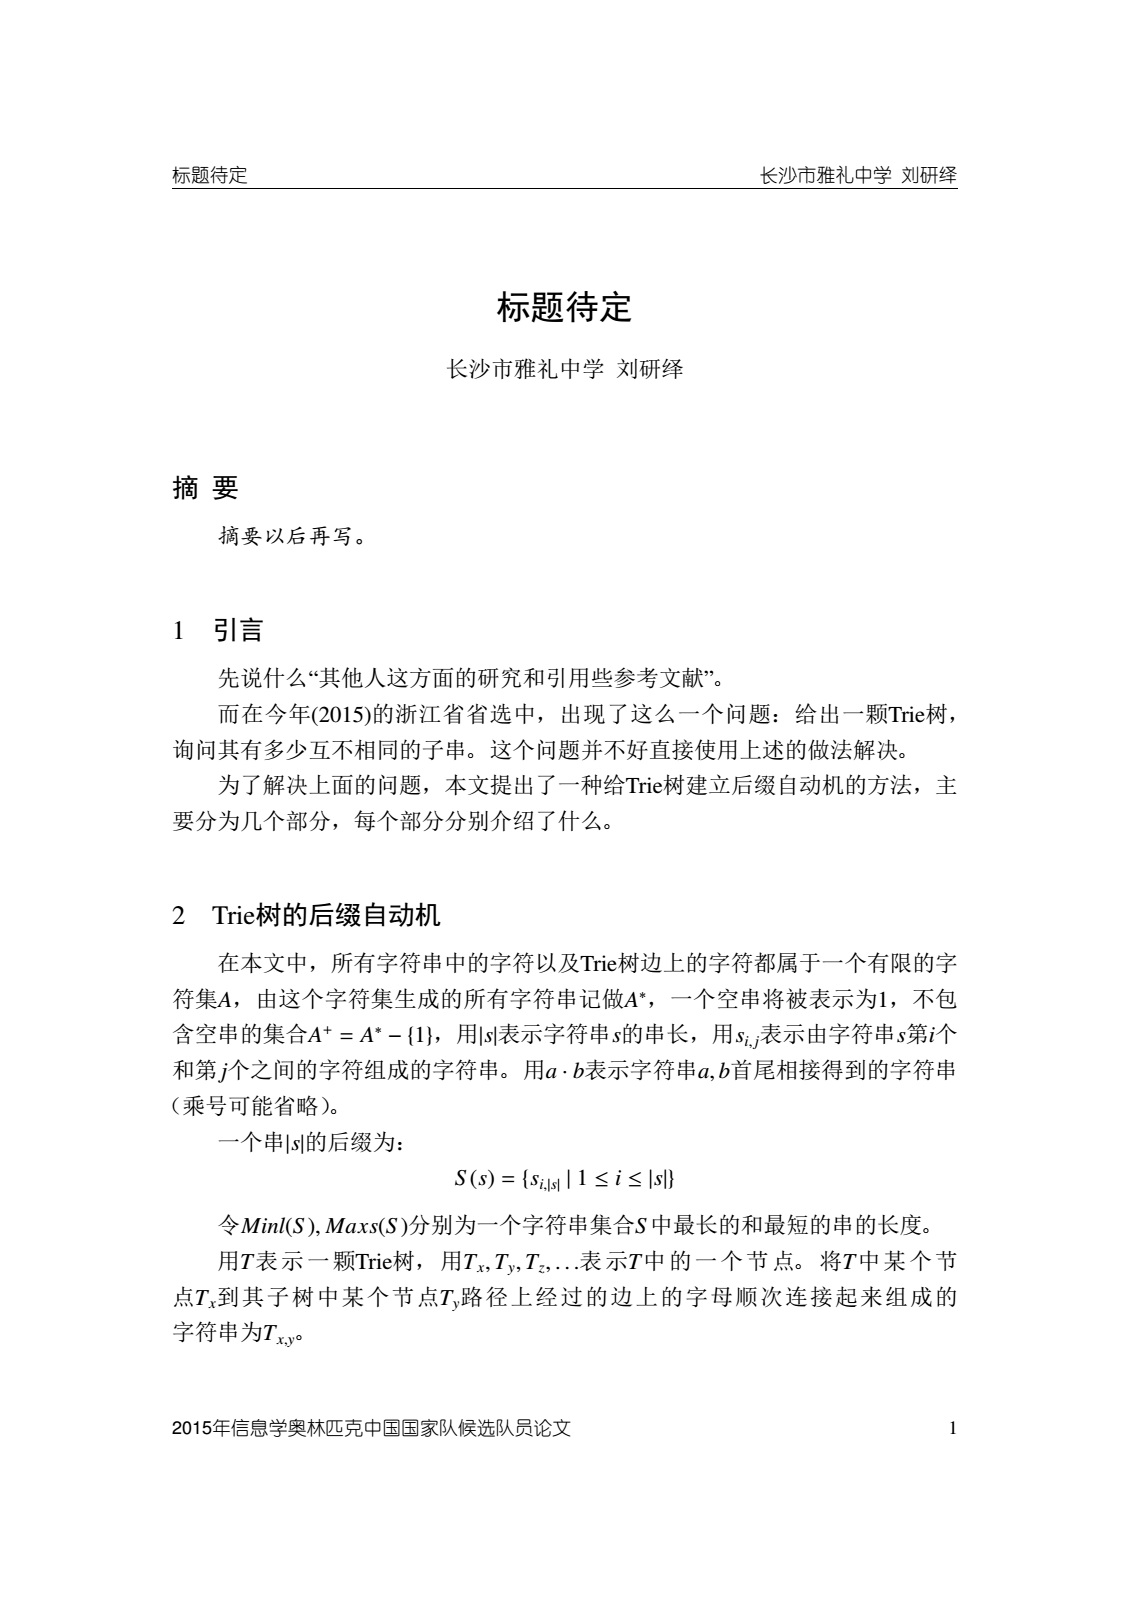
\includegraphics[width= 6.5cm]{1.jpg}
					\caption{一个例子}
				\end{wrapfigure}
				母和一个正号或负号。规定两个正
				方形能相拼当且仅当公用一条边,其均不是两个零,且字母相等,负号相反。正方形可旋转翻转,求是否存在一种拼法使得这个组合物想有多大,就能有多大。
				
				右图为一种可能的情况的拼接方案,但仅使用这些型号的正方形,只能拼出有限大小的组合物。
				
				$N \le \num{40000}$。
			
			\subsubsection{算法讨论}
				注意到,如果存在一个正方形序列链 $P_1, P_2, \ldots P_n, P_1$,两两前后拼接成链,那么可以通过翻转正方形的方式,使得这条链从左上只向右和下延伸。将翻转后的链复制任意多份,首尾拼接再按上述方式翻转,就能够构造出足够大的组合物,此时答案为是;反之,若不存在,则答案显然为否。问题即,询问是否存在这样的链。
				
				四边的标志总共有 $2 \times 26 + 1 = 53$ 种,对于每个标志可建一个对应的结点,构成图。
				对于一个四边标志为 $a,b,c,d$ 的正方形,在图上表示为 $a \rightarrow \bar{b}, a \rightarrow \bar{c}, a \rightarrow \bar{d}, b \rightarrow \bar{a}, b \rightarrow \bar{c}, \ldots, d \rightarrow \bar{c}  $ 等 $12$ 条边(两个零对应的结点不参与连边),其中 $\bar{x}$ 表示 $x$ 结点对应字母相等符号相反的结点。答案取决于是否有长度不低于 $1$ 的有向环。运行 Tarjan 算法即可求解。
			\subsubsection{时空复杂度}
				时间复杂度 $\mathcal{O}\left(|\varSigma|+N\right) = \mathcal{O}\left(N\right)$。$|\varSigma|$ 为大写字母数。
				
				空间复杂度 $\mathcal{O}\left(|\varSigma|\right) = \mathcal{O}\left(1\right)$。
		
		
		
			
		\newpage
		\subsection{ACM/ICPC World Finals 2013 C Surely You Congest}
			\subsubsection{题目大意}
				给定无向图 $G = (V,E)$。边有边权 $ W:E \mapsto \mathbb{R}_+$,表示经过该边的时间。$K$ 个人从不同的结点同时出发,欲沿最短路前往 $1$ 号结点。设计一种方案,使得不会有两个人,同时从某条道路的一端出发,同时到达另一端,且使尽可能多的人
				到达  $1$ 号结点。输出该人数。
				
				结点数 $N = |V| \le \num{25 000},$ 边数 $ M = |E| \le \num{50 000},$ 人数 $K \le \num{1 000}, \forall e \in E, $ 边权 $W(e) \le \num{10 000}$。
			\subsubsection{算法讨论}
				根据图论知识,如果边 $ e = (u,v)$  满足 $d(u) = W(e) + d(v)$,其中 $d(x)$ 表示结点 $x$ 到 $1$ 号结点的最短路长度,那么各人是有可能从 $u$ 到 $v$ 地经过这条边的;反之若  $d(u) \ne W(e) + d(v)$,则各人一定不会经过这条边。故我们可以先用堆优化的 Dijkstra 算法预处理出 $d(\cdot)$。
				
				再次使用图论知识,进一步分析可知,如两个人出发时所在结点到 $1$ 号结点的最短距离不同,那么他们一定不会产生冲突;而若两个人的出发结点到 $  1$ 号结点的最短距离相同,那么是否产生冲突就取决于是否经过了同一条边。因此我们可以对各个距离上的人分开处理。对于每一组人,则要求在两两间不经过同一条边,且均走最短路的条件下,最大化抵达 $1$ 号结点的人数。
				
				该问题可用最大流算法解决。添加一个虚拟结点 $s$,即新点集 $V^\prime = V \cup \{s\}$。对于该组所在的每一个人所在的结点 $i$, 加边 $(s,i),$容量$ f(s,i) = 1$。而对于原图中满足 $d(u) = W(e) + d(v)$ 的边 $e=(u,v)$,在网络中加
				边 $(u,v),$容量$f(u,v)=1$。设 $t = 1$ 号结点。那么网络 $\textstyle G^\prime = (V^\prime,E^\prime), E^\prime = \bigcup_{i} (s,i) \cup \bigcup_{d(u) = W(e) + d(v)} e  $ 关于容量 $f$ 的 $s-t$ 最大流就是这一组问题的答案。累加求和。
				
				在实践中,SAP 算法和 Dinic 各有优势,亦各有劣势。在这里,笔者将这两者结合起来,先使用一定时间运行 SAP 算法,若该阶段 SAP 算法出解,则累计入答案;若 SAP 算法超时,那么转用 Dinic 算法,继续计算。在该题中,该方法可以避免超时问题。
			\subsubsection{时空复杂度}
				时间复杂度 $\mathcal{O}\left(N+M \log M + K\! \cdot\! Maxflow(N,M+N)\right)$。其中 $ Maxflow(N,M))$ 表示解决 $N$ 个点, $M$ 条有向边的网络流问题的复杂度。该上限非常宽松,实际情况远远达不到该复杂度。
				
				空间复杂度 $\mathcal{O}\left(N+M\right)$。
		\newpage
		\subsection{ACM/ICPC World Finals 2013 D Factors}
			\subsubsection{题目大意}
			设 $f(x)$ 表示将整数 $x,x>1$ 唯一分解后,重新排列的方案数。例如 $f(10) = 2$ 因为 \begin{align} 10 & = 2 \cdot 5 = 5 \cdot 2 \intertext{$f(20) = 3$ 因为}  20 & = 2 \cdot 2 \cdot 5 = 2 \cdot 5 \cdot 2 = 5 \cdot 2 \cdot 2 \end{align}
			
			给定整数 $k$,求最小的 $f^{-1}(k)$,其中 $f^{-1}(x)$ 表示 $f(x)$ 的反函数
			。
			
			如最小的 $f^{-1}(1)=2,f^{-1}(2)=6,f^{-1}(3)=12,f^{-1}(105)=720$。
			
			$k < 2^{63}, $最小的 $f^{-1}(k) < 2^{63}$。多组询问。
			
			\subsubsection{算法讨论}
				由组合数学知识可知,设 $x = 2^{a_1} \cdot 3^{a_2} \cdot 5^{a_3} \cdot \cdots \cdot {p_k}^{a_k}$,其中 $p_k$ 表示第 $k$ 大的质数,则 
				\begin{align}
					f(x) = \binom{a_1 + a_2 + \cdots + a_k}{a_1, a_2, \ldots , a_k}
				\end{align}
				而如果将指数 $a_1, a_2, \ldots , a_k$ 从大到小排序为 $b_1, b_2, \ldots , b_k$,那么多项式系数 $\textstyle \binom{b_1 + b_2 + \cdots + b_k}{b_1, b_2, \ldots , b_k}$ 不会改变,即 $y = 2^{b_1} \cdot 3^{b_2} \cdot \cdots \cdot {p_k}^{b_k} \le x$ 且 $f(x) = f(y)$。故最小的 $f^{-1}(k)$ 在唯一分解后,随着质数底数的增加,指数不会上升。而满足该条件且低于 $2^{63}$ 的数非常有限,只有 \num{43607} 个,可以通过暴力搜索全部求出。找出这些数 $x$ 后,易求出其 $f(x)$ 并哈希。对于各关键字,保留最小的 $x$。最后,对于询问 $k$,在哈希表中找出答案输出即可。
			 	
				特殊处理 $f^{-1}(1)$。
			\subsubsection{时空复杂度}
				时间复杂度 $\mathcal{O}\left(g(k)\right)$。
				
				空间复杂度 $\mathcal{O}\left(g(k)\right)$。$g(k)$ 表示不超过 $k$ 且唯一分解后,随着质数底数的增加,指数不会上升的数的个数。 $g(2^{63}-1) = \num{43607}$。
			
		\newpage
		\subsection{ACM/ICPC World Finals 2013 E Harvard}
			\subsubsection{题目大意}
				有 $N$ 个内存池,各内存池有 $M$ 字节。若需访问 $1$ 号内存池里的数据,则可以直接使用 $1$ 单位的时间来完成。而若访问其他内存池中的数据,则需事先将 $BMR$ 改为该内存池的编号,再用 $1$ 单位予以访问。$BMR$ 是在其他地方存储的变量,修改其值耗费 $1$ 单位时间。
			
				现在有一个程序,包括循环语句和先后待访问的变量(变量均只有一字节),循环语句可嵌套。请合理分配该程序中的变量在内存中的位置,使得读取内存的时间最小化。
				
				变量数 $K \le \min (N\cdot M, 13), N,M \le 13$。程序源代码包含不超过 \num{1000} 个关键字(变量,循环标志)。总共要访问变量的次数不超过 \num{1e12}。
			\subsubsection{算法讨论}
				暴力搜索各变量的位置,并加以检验,取最优值。
				
				有一些有效的剪枝。
				\begin{enumerate}
					\item 分析可知,第一块内存应该尽可能的存储变量,因为其访问时间最少。先暴力搜索哪些变量进入了第一块内存池。
					\item 确定了第一块内存池中的元素后,将其从展开的程序中剔除,并统计相邻的变量各有多少。对于不在同一组内存池中的变量,其对答案的贡献值为在程序中相邻出现的次数。统计过程可用栈结构实现。
					\item 各个内存池内的元素的顺序不会影响结果,故可以规定,各内存池按从小到大的顺序搜索。
					\item 各个内存池的顺序不会影响结果,故可以规定,内存池按最大值从小到大的顺序搜索。
				\end{enumerate}
			
				设程序总共访问 $X$ 次变量。如果在枚举第一块内存池时,全部变量都进入了其中,则该情况答案为 $X$;否则,答案为 $(X + 1 + \text{剔除第一块内存后,相邻元素不在同一组的情况数})$。
			\subsubsection{时空复杂度}
				时间复杂度涉及到比较麻烦的组合数学的计算,并且上述减枝可能带来更低的上限,难以估算。但对于本题,该算法效率还算较高。
				
				空间复杂度 $\mathcal{O}\left(1\right)$。
				
		\newpage
		\subsection{ACM/ICPC World Finals 2013 F Low Power}
			\subsubsection{题目大意}
				有 $N$ 张 $2 \times K$ 的表格 $K_1,K_2, \ldots, K_N$。设 $f(A)$ 表示表格 $A$ 的第一行的最小值与第二行最小值之差的绝对值。求将 $2 N \times K$ 个数一对一的填入表格中,使得 $\textstyle \min_{i=1}^{n} f(K_i)$ 最小化。
				
				$2N \times K \le \num{1e6}$,待填入的数均为正整数,不超过 \num{1e9}。
			\subsubsection{算法讨论}
				不妨设各行最小的数从小到大排序后为 $a_1,a_2, \ldots a_{2N}$。
				\begin{theorem}
					存在一个最优解,一定是 $a_1,a_2$ 在同一个表格,$a_3,a_4$ 在同一个表格,……,$a_{2N-1},a_{2N}$ 在同一个表格。 \label{2013f1}
				\end{theorem}
				\begin{pf}
					调整法,如果当前的布局不是这样,那么必然存在 $i<j<p<q$,使得 $a_i,a_p$ 在一个表格, $a_j,a_q$ 在另一个表格。若以行为整体,调整为 $a_i,a_j$ 分一组,$a_p,a_q$ 分一组,那么两个表格的 $f$ 值都不会增加,即答案 $\textstyle \min_{i=1}^{n} f(K_i)$ 也不会增加。重复迭代上述过程,即可得到最终的布局,且该布局优于其他的任意布局。\qed
				\end{pf}
				\begin{theorem}
					存在一个最优解,同一表格中两行的最小值在即将填入的数中大小一定相邻。
				\end{theorem}
				\begin{pf}
					调整法,如果 $a_{2i-1}, a_{2i}$ 在同一个表格,且在即将填入的数字从小到大排序后形成的序列中,与 $a_{2i-1}$ 相邻的数为 $x$,其中 $x$ 在 $a_{2i-1}$ 之后,位置上异于 $a_{2i}$。根据定理  \ref{2013f1},$x$ 一定在其所在行中不是最小值,且 $a_{2i-1} \le x \le a_{2i}$。强制交换 $x$ 和 $a_{2i}$ 后,由于  $x \le a_{2i}$,故原先 $x$ 所在行的最小值不会变化,而原先 $a_{2i}$  所在行的最小值会变为 $x$,故原先 $a_{2i}$  所在的表格的 $f$ 值不会上升。反复迭代可知,大小相邻的数作为最小值不会比其他策略的值更差。\qed
				\end{pf}
				至此,可以使用二分和贪心策略解决问题。设当前猜测答案为 $K_{\text{ans}}$。那么将要填入的序列排序后扫描,若相邻的两个数相差不超过 $K_{\text{ans}}$,那么肯定可以用一张新的表格将这两个数作为最小值填入,原因是如果这样做都无解的话,那么其他填法也肯定无解,这其中有一个蕴含的关系。否则,若相邻的两个数相差大于 $K_{\text{ans}}$,则将扫描序列中最小的数填入先前的某张表格中作为较大值。如果该步骤没有空位能够容纳该值,则返回无解。若填满了 $N$ 张表格,则返回有解。使用二分算法即可在对数时间内得知答案。
			\subsubsection{时空复杂度}
				时间复杂度 $\mathcal{O}\left(N\cdot K \log M \right)$。$M$ 是待填入的数的数据规模。本题 $M = \num{1e9}$。
			
				空间复杂度 $\mathcal{O}\left(N\cdot K \right)$。
		\newpage
		\subsection{ACM/ICPC World Finals 2013 H
				Матрёшка
			}
			\subsubsection{题目大意}
				$N$ 个套娃排成一排,%大小不一,
				第 $i$ 个的大小为 $A_i$。现在要将其中一些套在一起,合并成若干个大套娃。要求
				\begin{enumerate}
					\item 整个过程只能是较大的套娃套较小的套娃。
					\item 每次只能将相邻两个套娃(可能是已经合并过的),通过打开和关闭盖子的方式将其套成(合并为)一个更大的套娃。
					\item 最终每个大套娃是由大小为 $1,2,3, \ldots, x$ 的套娃相套而成,$x$ 是大套娃所含的最小单位的套娃数。
				\end{enumerate}
				打开和关闭盖子的时间为 1。试问完成任务的最少时间。
				
				$N \le 500, 1\le  A_i \le 500,  A_i $ 为整数。
			\subsubsection{算法讨论}
				设将 $L$ 到 $R$ 的套娃套成一个单独的大套娃的时间为 $C[L][R]$,再设设处理好前 $i$ 个套娃的最少时间为 $F[i]$。那么使用时间复杂度 $\mathcal{O}\left(N^3\right)$ 的动态规划
				\begin{align}
					F[i] & = \min_{1 \le j \le i \atop \text{$j$ 到 $i$ 合并满足要求}%\{ A_j, A_{j+1}, \ldots, A_{i}\} = [1,j-i+1] \cap \mathbb{Z}
					}
					F[j-1] + C[j][i]
					\intertext{边界}
						F[0]& =0
				\end{align}
				即可求出答案 $F[N]$。下求 $C[L][R]$。
				
				同样可以使用动态规划求出,
				\begin{align}
					C[L][R] = \min_{L \le i < R}{ C[L][i] + C[i+1][R] +  W(L,i,R)}
				\end{align}
				其中 $W(L,i,R)$ 表示合并好 $L$ 到 $i$ 以及 $(i+1)$ 到 $R$ 的套娃后,仅合并这两者的最少所需时间。设 $k$ 为最小值较小的一堆套娃中,尺寸低于
				另一堆
				最小值的套娃数,那么 $W(L,i,R) = R-L+1-k$。
				忽略 $W(\cdot,\cdot,\cdot)$ 	 的计算时间,该动态规划的时间复杂度%为
				  $\mathcal{O}\left(N^3\right)$ 。
				
				而 $W(\cdot,\cdot,\cdot)$ 也
				可以用均摊 $\mathcal{O}\left(1\right)$ 时间求出。不失一般性,设 $L$ 到 $i$ 尺寸的最小值相对较大,为 $MinValue$,另一种情况对称处理。不妨动态维护 $(i+1)$ 到 $R$ 的套娃中,各个尺寸 $x$ 的套娃数 $H[x]$。对于每个 $i$ 的遍历值,$H\left(\cdot\right)$只需修改一个数,可以均摊 $\mathcal{O}\left(1\right)$ 算出。而 $\textstyle W(L,i,R) = \sum_{j=1}^{MinValue-1} H[j]$。根据 $MinValue$ 与 $A[i]$ 的关系,若 $MinValue>A[i]$ 则 $ W $函数的值较原来自减一,否则保持原样,也可以在 $\mathcal{O}\left(1\right)$ 时间维护好 $W(L,i,R)$。
				另一方面,$i$ 从 $L$ 枚举到 $(R - 1)$ 的过程中,前者的最小值  $MinValue$ 也会发生变化,且不断地减小。若  $MinValue$ 从 $x$ 减少到 $(x -1)$,那么 $W$ 函数较原来会自减 $H[x-1]$。$MinValue$ 的值只可能从 $(R-L+1)$ 减少到 $1$,减少次数不会超过  $(R-L+1)$ ,故也可以在均摊 $\mathcal{O}\left(1\right)$ 时间维护好 $W(L,i,R)$。
				综上,整个算法的时间复杂度可控制在 $\mathcal{O}\left(N^3\right)$ 。
			\subsubsection{时空复杂度}
				时间复杂度 $\mathcal{O}\left(N^3\right)$。
				
				空间复杂度 $\mathcal{O}\left(N^2\right)$。
			
		\newpage
		\subsection{ACM/ICPC World Finals 2013 I Pirate Chest}
			\subsubsection{题目大意}
				在 $N \times M$ 的网格状池塘里放入底部尺寸不超过 $P \times Q$ 的箱子,高度任意,但放入后其顶部的高度必须严格低于水面,并且长宽高为整数,与网格对齐。任意一个网格内池塘的底部平齐,深度由 $N \times M$ 的深度矩阵 $A$ 给出。 
				试最大化箱子的体积。
				
				$N,M \le 500, A_{i,j} \le \num{1e9}, A_{i,j}$ 为非负整数。
			\subsubsection{算法讨论}
				不妨先考虑一个一维版本的问题,即  $N = 1$ 的情况。假设箱子跨过了 $(1,i)$ 的格子,且它是所有被覆盖的格子中,深度最浅的。那么箱子的
				高度 $h$ 应当满足
				\begin{align}
					h& < \frac{Sh}{N \times M} + A_{i,j}
					\intertext{即}
					h &< \frac{A_{i,j}\times N \times M}{N \times M - S}\\
					h &= \left\lceil{(A_{i,j} \times N \times M)} / {(N \times M - S)} \right\rceil -1 \label{Piratecalc}
				\end{align}	
				其中 $S$ 为箱子底部的真实表面积。而箱子体积 $V = Sh$,由此可见,$S$ 应当尽可能的大。
				
				可以使用单调栈预处理出 $l_i$,表示最大的 $j, j<i$ 使得 $A_{1,j}<A_{1,i}$,以及 $r_i$,最小的 $j, j> i$ 使得 $A_{1,j}<A_{1,i}$。那么所有满足 $(1,i)$ 为被覆盖的格子中,深度最浅的摆放方法中,最大的底面积为 $S = \min( r_i - l_i -1 ,Q)$。代入 \eqref{Piratecalc} 即可求得高度 $h$ 和 体积 $V$。该子问题时间复杂度 $\mathcal{O}\left(M\right)$。
				
				对于原问题,不妨枚举箱子所跨的行,再合并成一行,使用上述的方法求得最大体积,取最优值,就可以求得答案。
				注意到 $P \times  Q$ 的尺寸可以旋转,故还需交换 $P, Q$ 的值再计算一次。
				仅枚举跨越的行复杂度为 $\mathcal{O}\left(N \cdot M\right)$。
				
			\subsubsection{时空复杂度}
				时间复杂度 $\mathcal{O}\left(N\cdot M^2\right)$。
					
				空间复杂度 $\mathcal{O}\left(N\cdot M\right)$。\newpage
		\subsection{ACM/ICPC World Finals 2013 J Pollution Solution}
			\subsubsection{题目大意}
				求半圆
				\begin{align}
					R: x^2+y^2 \le r^2 \land y>0
				\end{align}
				与简单多边形交的面积。
				
				简单多边形的点数 $N \le 100$,且总在 $x$ 轴上方。
			
			\subsubsection{算法讨论}
				如图 \ref{convert},求多边形面积时,我们可以转化为求 $N$ 个有向三角形的面积之和。此题也可借鉴该思想。
				\begin{figure}[!htb]
				\centering
				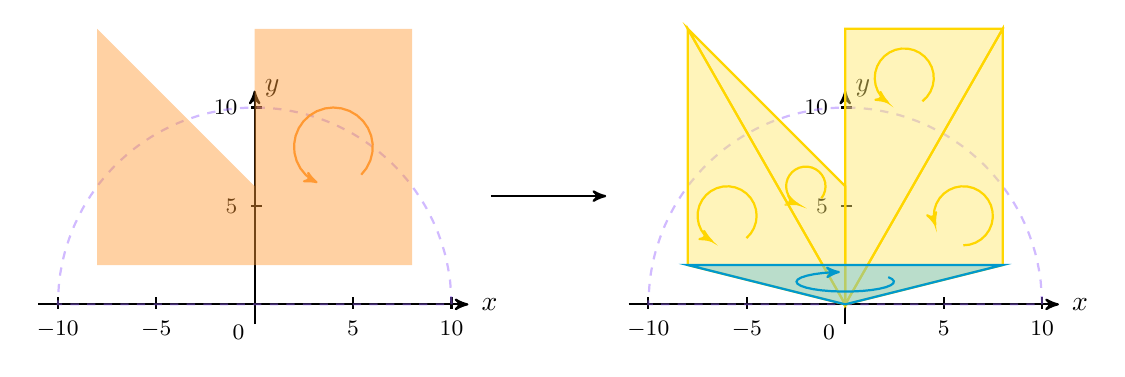
\begin{tikzpicture}[shorten >=1pt,node distance=2cm,on grid,>=stealth',thick,
					every state/.style={fill,draw=none,orange,text=white!80!orange,circular drop shadow},
					accepting/.style ={green!50!black,text=green!50!black!20!white},
					initial/.style ={red,text=white!80!red},scale= 0.25 ]
					\definecolor{qqzzcc}{rgb}{0,0.6,0.8}
					\definecolor{ffdxqq}{rgb}{1,0.84,0}
					\definecolor{zzwwff}{rgb}{0.6,0.4,1}
					\definecolor{ffttww}{rgb}{1,0.2,0.4}
					\definecolor{ffzzzz}{rgb}{1,0.6,0.6}
					\definecolor{ffzztt}{rgb}{1,0.6,0.2}
					
					\draw[->] (-11,0) -- (11,0) node[right] {$x$};	
					\draw[->] (0,-1) -- (0,11) node[right] {$y$};
					\foreach \x in {-10,-5,5,10}
					\draw[shift={(\x,0)},color=black] (0pt,10pt) -- (0pt,-10pt) node[below] {\footnotesize $\x$};		
					\draw[color=black] (0pt,-40pt) node[left] {\footnotesize $0$};
					\foreach \y in {5,10}
						\draw[shift={(0,\y)},color=black] (10pt,0pt) -- (-10pt,0pt) node[left] {\footnotesize $\y$};
%					\draw[dashed] (0,0) -- (2,0);
%					\draw[dashed] (0,1) -- (2,1);
%					\draw[dashed] (0,2) -- (2,2);
%					\draw[dashed] (0,0) -- (0,2);
%					\draw[dashed] (1,0) -- (1,2);
%					\draw[dashed] (2,0) -- (2,2);
					\draw[draw = zzwwff,dashed, fill = none,smooth,domain=0:180,opacity = 0.45] (10,0) -- plot({10*cos(\x)},{10*sin(\x)}) -- cycle;
					
					\draw[draw = none, fill = ffzztt,smooth,domain=0:90,opacity = 0.45] (8,2) --
						(8,14) --
						(0,14) --
						(0,6) --
						(-8,14) --
						(-8,2) -- cycle;

					\draw[->,color=ffzztt, fill = none,domain=-90:205]  plot({4+2*cos(\x+45)},{8+2*sin(\x+45)}) ;
					
										
%					\draw[draw = none, fill = qqzzcc,smooth,domain=0:90,opacity = 0.45] (0,0) -- (1,0) -- plot({2-cos(\x)},{sin(\x)})  -- (2,2) -- (1,2) --  plot({cos(\x)},{2-sin(\x)}) -- cycle;
					
%					\draw[line width=1pt,smooth,domain=0:90] plot({cos(\x)},{2-sin(\x)});
%					\draw[line width=1pt,smooth,domain=0:90] plot({2-cos(\x)},{sin(\x)});
					\draw[->] (12,5.5) -- (18,5.5);
					\begin{scope}[xshift=30 cm]
					
					\draw[->] (-11,0) -- (11,0) node[right] {$x$};	
					\draw[->] (0,-1) -- (0,11) node[right] {$y$};
					\foreach \x in {-10,-5,5,10}
					\draw[shift={(\x,0)},color=black] (0pt,10pt) -- (0pt,-10pt) node[below] {\footnotesize $\x$};		
					\draw[color=black] (0pt,-40pt) node[left] {\footnotesize $0$};
					\foreach \y in {5,10}
						\draw[shift={(0,\y)},color=black] (10pt,0pt) -- (-10pt,0pt) node[left] {\footnotesize $\y$};
%					\draw[dashed] (0,0) -- (2,0);
%					\draw[dashed] (0,1) -- (2,1);
%					\draw[dashed] (0,2) -- (2,2);
%					\draw[dashed] (0,0) -- (0,2);
%					\draw[dashed] (1,0) -- (1,2);
%					\draw[dashed] (2,0) -- (2,2);
					\draw[draw = zzwwff,dashed, fill = none,smooth,domain=0:180,opacity = 0.45] (10,0) -- plot({10*cos(\x)},{10*sin(\x)}) -- cycle;
					\draw[draw = ffdxqq, fill = ffdxqq!60!white,smooth,domain=0:90,fill opacity = 0.45] 
						(0,0) -- (8,2) --  (8,14) -- cycle;
					\draw[color = ffdxqq,->, domain=-90:205]  plot({6+1.5*cos(\x)},{4.5+1.5*sin(\x)}) ;
					
					\draw[draw = ffdxqq, fill = ffdxqq!60!white,smooth,domain=0:90,fill opacity = 0.45] 
						(0,0) -- (8,14) -- (0,14) -- cycle;
					\draw[color = ffdxqq,->, domain=-90:205]  plot({3+1.5*cos(\x+38)},{11.5+1.5*sin(\x+38)}) ;
					
					\draw[draw = ffdxqq, fill = ffdxqq!60!white,smooth,domain=0:90,fill opacity = 0.45] 
						(0,0) -- (0,14) --  (0,6) -- cycle;

					\draw[draw = ffdxqq, fill = ffdxqq!60!white,smooth,domain=0:90,fill opacity = 0.45] 
						(0,0) -- (0,6) --  (-8,14) -- cycle;
					\draw[color = ffdxqq,->, domain=-90:205]  plot({-2+1*cos(\x+52)},{6+1*sin(\x+52)}) ;
					\draw[draw = ffdxqq, fill = ffdxqq!60!white,smooth,domain=0:90,fill opacity = 0.45] 
						(0,0) -- (-8,14) --  (-8,2) -- cycle;
					\draw[color = ffdxqq,->, domain=-90:205]  plot({-6+1.5*cos(\x+41)},{4.5+1.5*sin(\x+41)}) ;
					\draw[draw = qqzzcc, fill = qqzzcc!60!white,smooth,domain=0:90,fill opacity = 0.45] 
						(0,0) -- (-8,2) --  (8,2)  -- cycle;
					\draw[color = qqzzcc,->, domain=-90:205]  plot({1.5*1.65*cos(-\x-62)},{1.15+0.5*sin(-\x-62)}) ;
										
%					\draw[draw = none, fill = qqzzcc,smooth,domain=0:90,opacity = 0.45] (0,0) -- (1,0) -- plot({2-cos(\x)},{sin(\x)})  -- (2,2) -- (1,2) --  plot({cos(\x)},{2-sin(\x)}) -- cycle;
					
%					\draw[line width=1pt,smooth,domain=0:90] plot({cos(\x)},{2-sin(\x)});
%					\draw[line width=1pt,smooth,domain=0:90] plot({2-cos(\x)},{sin(\x)});
					
					
					\end{scope}
				\end{tikzpicture}
			\caption{ 转为有向三角形(黄正蓝负) } \label{convert}
			\vspace{-1em}
			\end{figure}
			
			如图 \ref{add},先求出各线段与圆的交点。方法是将每一段线段写为参数方程 $\mathbf{p} = \mathbf{a} + \mathbf{v}t , 0 \le t \le 1$,代入圆方程 $\mathbf{p}^2 = r^2$,解关于参数 $t$ 的一元二次方程$(\mathbf{a} + \mathbf{v}t)^2 = r^2$,代回参数方程求得交点。再将这些交点插入到多边形顶点序列中。这样做的好处是,多边形的本质未改变,而相邻点间的线段要么全部位于圆内,要么全部位于圆外。而具体是在圆内还是圆外,可通过线段中点到原点的距离与半径的关系来判断。
			
			
			\begin{figure}[!htb]
				\centering
				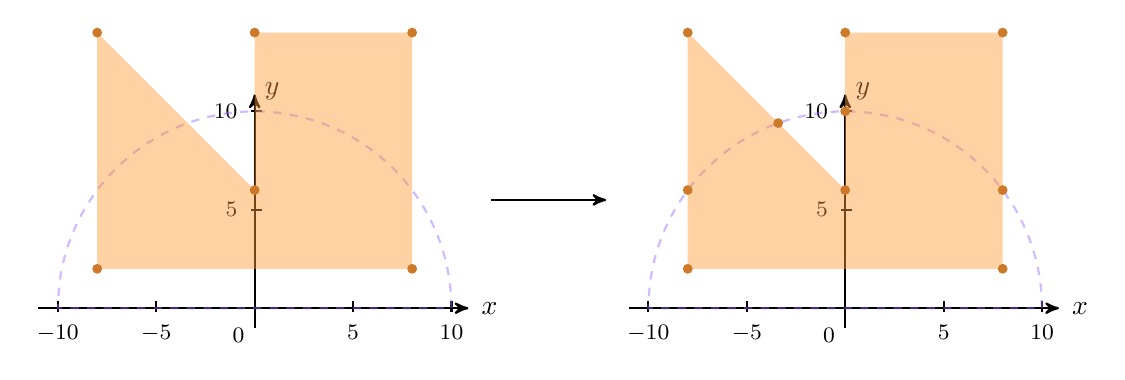
\begin{tikzpicture}[shorten >=1pt,node distance=2cm,on grid,>=stealth',thick,
					every state/.style={fill,draw=none,orange,text=white!80!orange,circular drop shadow},
					accepting/.style ={green!50!black,text=green!50!black!20!white},
					initial/.style ={red,text=white!80!red},scale= 0.25 ]
					\definecolor{qqzzcc}{rgb}{0,0.6,0.8}
					\definecolor{ffdxqq}{rgb}{1,0.84,0}
					\definecolor{zzwwff}{rgb}{0.6,0.4,1}
					\definecolor{ffttww}{rgb}{1,0.2,0.4}
					\definecolor{ffzzzz}{rgb}{1,0.6,0.6}
					\definecolor{ffzztt}{rgb}{1,0.6,0.2}
					
					\draw[->] (-11,0) -- (11,0) node[right] {$x$};	
					\draw[->] (0,-1) -- (0,11) node[right] {$y$};
					\foreach \x in {-10,-5,5,10}
					\draw[shift={(\x,0)},color=black] (0pt,10pt) -- (0pt,-10pt) node[below] {\footnotesize $\x$};		
					\draw[color=black] (0pt,-40pt) node[left] {\footnotesize $0$};
					\foreach \y in {5,10}
						\draw[shift={(0,\y)},color=black] (10pt,0pt) -- (-10pt,0pt) node[left] {\footnotesize $\y$};
%					\draw[dashed] (0,0) -- (2,0);
%					\draw[dashed] (0,1) -- (2,1);
%					\draw[dashed] (0,2) -- (2,2);
%					\draw[dashed] (0,0) -- (0,2);
%					\draw[dashed] (1,0) -- (1,2);
%					\draw[dashed] (2,0) -- (2,2);
					\draw[draw = zzwwff,dashed, fill = none,smooth,domain=0:180,opacity = 0.45] (10,0) -- plot({10*cos(\x)},{10*sin(\x)}) -- cycle;
					
					\draw[draw = none, fill = ffzztt,smooth,domain=0:90,opacity = 0.45] (8,2) --
						(8,14) --
						(0,14) --
						(0,6) --
						(-8,14) --
						(-8,2) -- cycle;
										
%					\draw[draw = none, fill = qqzzcc,smooth,domain=0:90,opacity = 0.45] (0,0) -- (1,0) -- plot({2-cos(\x)},{sin(\x)})  -- (2,2) -- (1,2) --  plot({cos(\x)},{2-sin(\x)}) -- cycle;
					
%					\draw[line width=1pt,smooth,domain=0:90] plot({cos(\x)},{2-sin(\x)});
%					\draw[line width=1pt,smooth,domain=0:90] plot({2-cos(\x)},{sin(\x)});
					\draw[->] (12,5.5) -- (18,5.5);
					
					
					\draw[fill=ffzztt!80!black,draw=none] (8,2) circle (0.25cm)
										(8,14) circle (0.25cm)
										(0,14) circle (0.25cm)
										(0,6) circle (0.25cm)
										(-8,14) circle (0.25cm)
										(-8,2) circle (0.25cm);
					\begin{scope}[xshift=30 cm]
					
					\draw[->] (-11,0) -- (11,0) node[right] {$x$};	
					\draw[->] (0,-1) -- (0,11) node[right] {$y$};
					\foreach \x in {-10,-5,5,10}
					\draw[shift={(\x,0)},color=black] (0pt,10pt) -- (0pt,-10pt) node[below] {\footnotesize $\x$};		
					\draw[color=black] (0pt,-40pt) node[left] {\footnotesize $0$};
					\foreach \y in {5,10}
						\draw[shift={(0,\y)},color=black] (10pt,0pt) -- (-10pt,0pt) node[left] {\footnotesize $\y$};
%					\draw[dashed] (0,0) -- (2,0);
%					\draw[dashed] (0,1) -- (2,1);
%					\draw[dashed] (0,2) -- (2,2);
%					\draw[dashed] (0,0) -- (0,2);
%					\draw[dashed] (1,0) -- (1,2);
%					\draw[dashed] (2,0) -- (2,2);
					\draw[draw = zzwwff,dashed, fill = none,smooth,domain=0:180,opacity = 0.45] (10,0) -- plot({10*cos(\x)},{10*sin(\x)}) -- cycle;
					
					\draw[draw = none, fill = ffzztt,smooth,domain=0:90,opacity = 0.45] (8,2) --
						(8,14) --
						(0,14) --
						(0,6) --
						(-8,14) --
						(-8,2) -- cycle;
					
					\draw[fill=ffzztt!80!black,draw=none] (8,2) circle (0.25cm)
										(8,14) circle (0.25cm)
										(0,14) circle (0.25cm)
										(0,6) circle (0.25cm)
										(-8,14) circle (0.25cm)
										(-8,2) circle (0.25cm)
										(-8,6) circle (0.25cm)
										(8,6) circle (0.25cm)
										(0,10) circle (0.25cm)
										(-3.403124,9.403124) circle (0.25cm);
										
										
%					\draw[draw = none, fill = qqzzcc,smooth,domain=0:90,opacity = 0.45] (0,0) -- (1,0) -- plot({2-cos(\x)},{sin(\x)})  -- (2,2) -- (1,2) --  plot({cos(\x)},{2-sin(\x)}) -- cycle;
					
%					\draw[line width=1pt,smooth,domain=0:90] plot({cos(\x)},{2-sin(\x)});
%					\draw[line width=1pt,smooth,domain=0:90] plot({2-cos(\x)},{sin(\x)});
					
					
					\end{scope}
				\end{tikzpicture}
			\caption{ 求交点,加点 } \label{add}
			\vspace{-1em}
			\end{figure}
				
			对于在圆内的部分,其对交面积的贡献为前后端点$(x_1,y_1),(x_2,y_2)$ 的叉积的一半 
			\begin{align}
				\frac{1}{2}(x_1,y_1) \times (x_2,y_2) = \frac{1}{2}x_1y_2-\frac{1}{2}x_2y_1
			\end{align}
			而在圆外的部分,对交面积的贡献实质为一个扇形的面积,有向圆心角的大小
			\begin{align}
				|\theta| = \arccos \frac{(x_1,y_1)  \cdot (x_2,y_2)}{\left|(x_1,y_1)\right|\!\!\, \cdot\!\!\, \left|(x_2,y_2)\right|}
						=  \arccos \frac{x_1x_2+y_1y_2}{\sqrt{\left(x_1^2+y_1^2\right)\!\!\, \cdot\!\!\, \left(x_2^2+y_2^2\right)}}
			\end{align}
			而其正负性与 $\left((x_1,y_1) \times (x_2,y_2)\right)$ 相同。代入扇形面积公式 $ \textstyle S = \frac{1}{2} \theta r^2$ 即为该线段对交面积的贡献。求和。
			\begin{figure}[!htb]
				\centering
				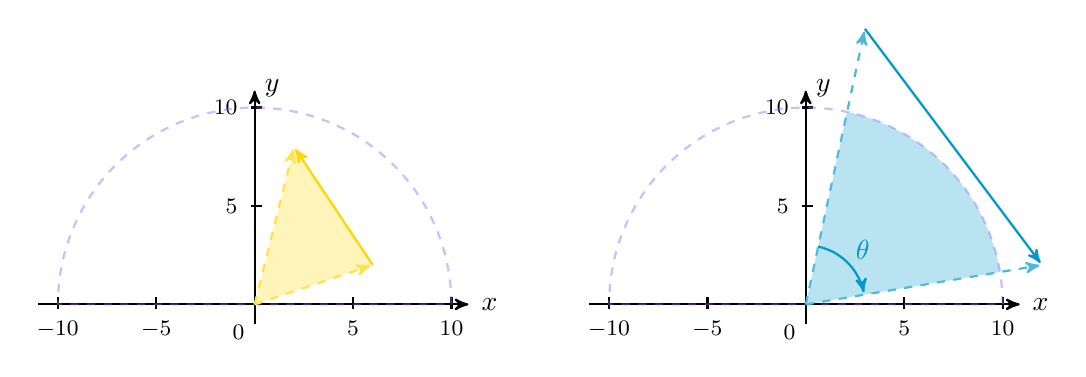
\begin{tikzpicture}[shorten >=1pt,node distance=2cm,on grid,>=stealth',thick,
					every state/.style={fill,draw=none,orange,text=white!80!orange,circular drop shadow},
					accepting/.style ={green!50!black,text=green!50!black!20!white},
					initial/.style ={red,text=white!80!red},scale= 0.25 ]
					\definecolor{qqzzcc}{rgb}{0,0.6,0.8}
					\definecolor{ffdxqq}{rgb}{1,0.84,0}
					\definecolor{zzwwff}{rgb}{0.6,0.4,1}
					\definecolor{ffttww}{rgb}{1,0.2,0.4}
					\definecolor{ffzzzz}{rgb}{1,0.6,0.6}
					\definecolor{ffzztt}{rgb}{1,0.6,0.2}
					
					\draw[->] (-11,0) -- (11,0) node[right] {$x$};	
					\draw[->] (0,-1) -- (0,11) node[right] {$y$};
					\foreach \x in {-10,-5,5,10}
					\draw[shift={(\x,0)},color=black] (0pt,10pt) -- (0pt,-10pt) node[below] {\footnotesize $\x$};		
					\draw[color=black] (0pt,-40pt) node[left] {\footnotesize $0$};
					\foreach \y in {5,10}
						\draw[shift={(0,\y)},color=black] (10pt,0pt) -- (-10pt,0pt) node[left] {\footnotesize $\y$};
%					\draw[dashed] (0,0) -- (2,0);
%					\draw[dashed] (0,1) -- (2,1);
%					\draw[dashed] (0,2) -- (2,2);
%					\draw[dashed] (0,0) -- (0,2);
%					\draw[dashed] (1,0) -- (1,2);
%					\draw[dashed] (2,0) -- (2,2);
					\draw[draw = zzwwff,dashed, fill = none,smooth,domain=0:180,opacity = 0.45] (10,0) -- plot({10*cos(\x)},{10*sin(\x)}) -- cycle;
					
					\draw[draw = none, fill = ffdxqq!60!white,smooth,domain=0:90,opacity = 0.45] (0,0) --
						(6,2) --
						(2,8) -- cycle;
					\draw[color = ffdxqq!70!white, ->, dashed] (0,0) -- (6,2);
					\draw[color = ffdxqq!70!white, ->,dashed] (0,0) -- (2,8);
					\draw[color = ffdxqq, ->] (6,2) -- (2,8);
										
%					\draw[draw = none, fill = qqzzcc,smooth,domain=0:90,opacity = 0.45] (0,0) -- (1,0) -- plot({2-cos(\x)},{sin(\x)})  -- (2,2) -- (1,2) --  plot({cos(\x)},{2-sin(\x)}) -- cycle;
					
%					\draw[line width=1pt,smooth,domain=0:90] plot({cos(\x)},{2-sin(\x)});
%					\draw[line width=1pt,smooth,domain=0:90] plot({2-cos(\x)},{sin(\x)});
%					\draw[->] (12,5.5) -- (18,5.5);
					
					
					\begin{scope}[xshift= 28cm]
					
					\draw[->] (-11,0) -- (11,0) node[right] {$x$};	
					\draw[->] (0,-1) -- (0,11) node[right] {$y$};
					\foreach \x in {-10,-5,5,10}
					\draw[shift={(\x,0)},color=black] (0pt,10pt) -- (0pt,-10pt) node[below] {\footnotesize $\x$};		
					\draw[color=black] (0pt,-40pt) node[left] {\footnotesize $0$};
					\foreach \y in {5,10}
						\draw[shift={(0,\y)},color=black] (10pt,0pt) -- (-10pt,0pt) node[left] {\footnotesize $\y$};
%					\draw[dashed] (0,0) -- (2,0);
%					\draw[dashed] (0,1) -- (2,1);
%					\draw[dashed] (0,2) -- (2,2);
%					\draw[dashed] (0,0) -- (0,2);
%					\draw[dashed] (1,0) -- (1,2);
%					\draw[dashed] (2,0) -- (2,2);
					\draw[draw = zzwwff,dashed, fill = none,smooth,domain=0:180,opacity = 0.45] (10,0) -- plot({10*cos(\x)},{10*sin(\x)}) -- cycle;
					
%					\draw[draw = none, fill = ffdxqq!60!white,smooth,domain=0:90,opacity = 0.45] (0,0) --
%						(12,2) --
%						(3,14) -- cycle;
					
					\draw[color = qqzzcc!70!white, ->, dashed] (0,0) -- (12,2);
					\draw[color = qqzzcc!70!white, ->,dashed] (0,0) -- (3,14);
					\draw[color = qqzzcc, ->] (3,14) -- (12,2);
					
					\draw[draw = none, fill = qqzzcc!60!white,smooth,domain=9.462322208025617391140070541742:77.905242922987898747566331385281,opacity = 0.45] (0,0) --
						plot({10*cos(\x)},{10*sin(\x)})
						-- cycle;
					
					\draw[color = qqzzcc, -> ,domain=77.905242922987898747566331385281:9.462322208025617391140070541742] 
						plot({3*cos(\x)},{3*sin(\x)});
					\node[color = qqzzcc] at ({4*cos(43.683782565506758069353200963511)},{4*sin(43.683782565506758069353200963511)}) {$\theta$};
					
%					\draw[draw = none, fill = qqzzcc,smooth,domain=0:90,opacity = 0.45] (0,0) -- (1,0) -- plot({2-cos(\x)},{sin(\x)})  -- (2,2) -- (1,2) --  plot({cos(\x)},{2-sin(\x)}) -- cycle;
					
%					\draw[line width=1pt,smooth,domain=0:90] plot({cos(\x)},{2-sin(\x)});
%					\draw[line width=1pt,smooth,domain=0:90] plot({2-cos(\x)},{sin(\x)});
					
					
					\end{scope}
				\end{tikzpicture}
			\caption{ 两种情况对面积的贡献} 
			\vspace{-1em}
			\end{figure}
			
			\subsubsection{时空复杂度}
				时间复杂度 $\mathcal{O}\left(N\right)$。
				
				空间复杂度 $\mathcal{O}\left(1\right)$。
		\newpage
		\subsection{ACM/ICPC World Finals 2013 K Up a Tree}
			\subsubsection{题目大意}
			在以下三段有问题的代码中
			\begin{multicols}{3}
				\begin{algorithm}[H]
				\caption{前序遍历}
				\label{}
					\begin{algorithmic}[1]
						\Function{Pre}{$x$}
							\State \Call{Print}{$x$}
							\State \Call{\fbox{ 甲 }}{$x$ 的左儿子}
							\State \Call{\fbox{ 乙 }}{$x$ 的右儿子}
						\EndFunction
					\end{algorithmic}
				\end{algorithm}
				\begin{algorithm}[H]
				\caption{中序遍历}
				\label{}
					\begin{algorithmic}[1]
						\Function{In}{$x$}
							\State \Call{\fbox{ 丙 }}{$x$ 的左儿子}
							\State \Call{Print}{$x$}
							\State \Call{\fbox{ 丁 }}{$x$ 的右儿子}
						\EndFunction
					\end{algorithmic}
				\end{algorithm}
				\begin{algorithm}[H]
				\caption{后序遍历}
				\label{}
					\begin{algorithmic}[1]
						\Function{Post}{$x$}
							\State \Call{\fbox{ 戊 }}{$x$ 的左儿子}
							\State \Call{\fbox{ 己 }}{$x$ 的右儿子}
							\State \Call{Print}{$x$}
						\EndFunction
					\end{algorithmic}
				\end{algorithm}
			\end{multicols}
			填入恰好两个 \Call{Pre}{} 恰好两个 \Call{In}{} 和恰好两个\Call{Post}{},使得存在一个树,分别调用这三个函数后,得到的先序中序后序遍历为给定的串,并使得输入的树的正确前序中序后序遍历的字典序最小化。
			
			$4 \le \text{给定串的长度} \le 26$。
			\subsubsection{算法讨论}
			填写源代码的情况数只有 $\textstyle \binom{6}{2,2,2} = 90$ 种,可先枚举。
			
			这样,问题简化为,固定代码,给定一个二叉树调用\Call{Pre}{}, \Call{In}{} 和 \Call{Post}{} 函数中某几个的输出,求字典序最小的树使其满足条件。
			
			不妨递归处理,枚举左儿和右儿的元素数量,就可以确定根以及左右儿调用\Call{Pre}{}, \Call{In}{} 和 \Call{Post}{} 某几个后的输出,且规模更小。继续分治处理即可。最后合并答案,选择一个字典序最小的树返回。边界条件为输出全部为空串,此时可直接返回空树。
			
			有一些有效的剪枝。
			\begin{enumerate}
				\item 对于同一棵树,若几个函数输出的长度不一,可直接返回无解。
				\item 对于同一棵树,若有结点在某些函数的输出中出现,而在另一些函数的输出中未出现,可直接返回无解。
				\item 在递归调用时,若对于一棵子树,运行相同的函数,得出的输出序列不同,可直接返回无解。
				\item 枚举左右儿元素数后,若输出序列确定的根不一,可直接跳过此次枚举。
				\item 若左右儿对应的子问题有一个无解,可直接跳过此次枚举。
				\item 记忆化搜索
			\end{enumerate}
%			可加快搜索效率。
			\subsubsection{时空复杂度}
				时间复杂度 $\mathcal{O}\left(N^5\right)$,使用这些减枝后,实际运行时间远远达不到这个上限。
					
				空间复杂度 $\mathcal{O}\left(N^4\right)$。使用压位,索引,垃圾回收等方式可以进一步减少空间占用。
		\newpage
	
	\section{ACM/ICPC World Finals 2012}
		\subsection{ACM/ICPC World Finals 2012 A Asteroid Rangers}
			\subsubsection{题目大意}
				三维空间上有 $N$ 个点,第 $i$ 个点在 $t$ 时刻的位置 $\mathbf{p}_i = (\mathbf{a}_i + \mathbf{v}_i t)$,其中 $\mathbf{a}_i,\mathbf{v}_i$ 为给定常向量。
				$N$ 个点两两有连边,权值为欧几里德距离。试问从 $t = 0 $时起,$N$ 个点的最小生成树会变化几次。
			
				$N \le 50$。任意时刻任意两个点不会重合。如果在 $t_0$ 时刻某棵树\emph{成为}了最小生成树,那么在接下来的 $10^{-6}$ 时间里,该树是唯一的最小生成树。初始时刻最小生成树唯一。多组询问。
			\subsubsection{算法讨论}
				考虑 Kruskal 算法求最小生成树的过程以及边权变化的连续性,显然,只有当两条边的权值相等时,才可能有新的最小生成树出现。不妨求出这些时刻,方法是解二次(可能会退化为一次或零次)方程 $\left(\mathbf{p}_u - \mathbf{p}_v\right)^2 = \left(\mathbf{p}_r - \mathbf{p}_s\right)^2$,其中 $(u,v),(r,s)$ 是正在考察的两条边。这些时间点有不超过 $2\binom{\binom{N}{2}}{2} = \mathcal{O}\left(N^4\right)$ 个。
				
				对于上面求出的每个时间 $t$,我们只需验证 $(t + \epsilon)$ 时最小生成树是否改变,此处 $\epsilon$ 可取 $\num{1e-8}$。如果改变,则答案增加一。
				
				存在一个减枝。注意到如果在 $t$ 时刻最小生成树发生改变,那么一定是将被超越的边当前正在最小生成树内,而将超越其的边目前不在最小生成树。若当前的情况不是这样,那么最小生成树肯定不会变化,可以直接忽略掉该时间点 $t$。
			\subsubsection{时空复杂度}
				时间复杂度 $\mathcal{O}\left(N^6\right)$。上述减枝的优化效果很好,实际情况远远达不到该上限。
					
				空间复杂度 $\mathcal{O}\left(N^4\right)$。
		\newpage
		\subsection{ACM/ICPC World Finals 2012 B Curvy Little Bottles}
			\subsubsection{题目大意}
				有一个瓶子,其侧面由多项式函数 $y=f(x)$ 在 $x \in \left[L,R\right]$ 上绕 $x$ 轴旋转 \SI{360}{\degree} 而成,而底部和顶部分别是半径为 $f(L), f(R)$ 的圆。试求
				\begin{enumerate}
					\item 其体积;
					\item 若每隔 $V_0$ 的体积就给瓶子贴上标签,问最底部的不超过 $k$ 个标签到瓶子底端的距离。
				\end{enumerate}
				
				多项式 $f(x)$ 的次数 $N$ 不超过 $10$。$\forall x \in \left[L,R\right], f(x) > 0$。$k = 8$。多组询问。
			\subsubsection{算法讨论}
				显然体积为 $\int_{L}^{R} \pi f(x)^2 dx$。 求出多项式 $f(x)$ 的平方的原函数 $F(x) = \int f(x)^2 dx = \sum_{i=1}^{2N+1} k_ix^i$,那么第一问体积
				\begin{align}
					\int_{L}^{R} \pi f(x)^2 dx = \pi \left(F(R) - F(L)\right)
				\end{align}
				
				第二问相当于解方程 $\pi \left(F(x) - F(L)\right) = \mathrm{C}_1$ 即 $F(x) = \mathrm{C}_2$,其中 $\mathrm{C}_1,\mathrm{C}_2$ 为常数。由于 $f(x)>0$,故 $F(x)$ 单调,使用二分法即可求解。
			\subsubsection{时空复杂度}
				单组测试时间复杂度 $\mathcal{O}\left(N^2 + k p N\right)$。$p$ 是二分时检验答案的次数,与精度相关。
					
				空间复杂度 $\mathcal{O}\left(N\right)$。
		\newpage
		\subsection{ACM/ICPC World Finals 2012 C Bus Tour}
			\subsubsection{题目大意}
				给定无向图 $G =(V,E)$,边有边权 $W : E \mapsto \mathbb{R}_+$,$V$ 中有一个源 $s$,有一个汇 $t$。请选择一个子集 $X \subset V \setminus \{ s,t\}$ 使得 $|X| = \lfloor (|V|-2)/2 \rfloor, Y = V \setminus \{ s,t\} \setminus X$,且使得路径 
				\begin{align}
					s \rightarrow X  \text{ 中的结点} \rightarrow Y \text{  中的结点} \rightarrow t \rightarrow X \text{ 中的结点}
				 \rightarrow Y \text{ 中的结点}   \rightarrow s  \label{2012cpath}
				\end{align} 的长度最小化。
				几次访问集合中的节点的先后任意,且同样的集合前后两次的顺序可以不同。 求此最小的长度。
			
				$|V| = N \le 20$。多组询问。
			\subsubsection{算法讨论}
				设 $F[p][S]$ 表示从 $s$ 出发,经过集合 $S$ 中的结点到达 $p$ 结点的最短路径长度,$G[p][S]$ 表示从 $t$ 出发,经过集合 $S$ 中的结点到达 $p$ 结点的最短路径长度。使用 Floyed 算法求出两两间的最短路后,容易使用 SCDP 求出这两个值。
				
				随后 \eqref{2012cpath} 被分为了几部分 
				\begin{align}
					p  = \; & s \rightarrow X\setminus\{p\} \rightarrow p  , p \rightarrow q , q \rightarrow Y\setminus\{q\} \rightarrow t, \notag \\ & t \rightarrow X\setminus\{u\} \rightarrow u,u\rightarrow v, v \rightarrow Y \setminus \{v\} \rightarrow s
				\intertext{对应的最短路径长度为 }
					d_p  =\;  &\min_{p\in X,q\in Y} \left(F[p][X] + d(p,q) + G[q][Y]\right)  + \notag \\ & \min_{u\in X,v\in Y} \left(G[u][X] + d(u,v) + F[v][Y]\right) 
				\end{align}
				其中 $d(\cdot,\cdot)$ 表示两点最短路长度。枚举所有的 $X,p,q,u,v$,取最小值作为答案。
				
				特殊处理 $N = 3$ 的情况。
			\subsubsection{时空复杂度}
				时间复杂度 $\mathcal{O}\left(N^22^N\right)$。
					
				空间复杂度 $\mathcal{O}\left(N2^N\right)$。
		\newpage

		\subsection{ACM/ICPC World Finals 2012 D
Fibonacci Words}
			\subsubsection{题目大意}
				设第 $i$ 个斐波纳契串为 $S(i)$,则 $S(0)=0, S(1) = 1$ 且
				\begin{align}
					S(i)=S(i-1)+S(i-2)
				\end{align}
				$+$ 表示字符串的连接。问字符串 $T$ 在 $S(N)$ 中出现了多少次。
			
				$N \le 100, |T| = M \le \num{100000}$。$|x|$ 表示字符串 $x$ 的长度。答案 $< 2^{63}$。多组询问。
			\subsubsection{算法讨论}
				动态规划,设 $F[i]$ 表示 $T$ 在 $S(i)$ 中出现的次数
				\begin{align}
					F[i] & = F[i-1] + F[i-2] + T \text{ 在 $S(i-1)$ 与 $S(i-2)$ 衔接的地方出现的次数}
				\intertext{这个衔接处出现的次数可通过将 $S(i-1)$ 长度最多不超过 $(M-1)$ 的后缀与  $S(i-2)$ 长度最多不超过 $(M-1)$ 的前缀连接起来,运行 KMP 算法求得。边界}
					F[0] &= [V = 0]\\
					F[1]& = [V = 1]
				\end{align}
			
				虽然答案保证  $< 2^{63}$,但 $|S(N)| $ 不一定低于 $2^{63}$,需要处理斐波纳契串长度溢出的问题。
			\subsubsection{时空复杂度}
				时间复杂度 $\mathcal{O}\left(NM\right)$。
					
				空间复杂度 $\mathcal{O}\left(M\right)$。
		\newpage

		\subsection{ACM/ICPC World Finals 2012 E Infiltration}
			\subsubsection{题目大意}
				求竞赛图 $G=(V, E)$ 的最小支配集。
			
				$N = |V| \le 75$。
			\subsubsection{算法讨论}
				可以构造一个大小为 $\mathcal{O}{\left(\log N\right)}$ 的解。由于是竞赛图,故总存在出度超过 $\frac{N-1}{2}$ 的点。选择该点,并将该点和它所指向的点都从原图剔除,这样原图的点数规模缩小为原来的 $\frac{1}{2}$。经过   $\mathcal{O}{\left(\log N\right)}$ 次操作后,图被删除为空图,而选出的点就是一个支配集,大小  $\mathcal{O}{\left(\log N\right)}$ 。 对于该题 $N \le 75$ 的情况,这个解的大小不超过 $6$。
				
				那么只需搜索是否存在低于上述构造解的方案。对于此题,搜索量不超过  $\binom{75}{5} = \num{17259390}$。
				
				可用位运算优化搜索过程。	
			
			\subsubsection{时空复杂度}
				时间复杂度 $\mathcal{O}\left( N ^{ \log_2 N}\right)$。
					
				空间复杂度 $\mathcal{O}\left(N^2\right)$。
		\newpage

		\subsection{ACM/ICPC World Finals 2012 F Keys}
			\subsubsection{题目大意}
				给定一些钥匙和钥匙环,有些已经套在一起。现在请通过解开钥匙(环)和将钥匙(环)套在一起的方法,将钥匙按指定的分法分给两个人,使得每个人只需拿走一串连好的钥匙环即可解决问题(如果该人需要拿钥匙)。请在最小化钥匙和钥匙环之间的捆绑(解绑)的情况下,最小化钥匙环之间的捆绑(解绑)的次数。
				
				\begin{figure}[!htb]
 					\centering
					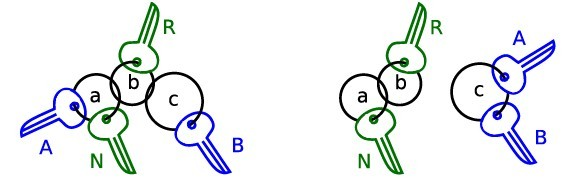
\includegraphics[width=0.8 \textwidth]{2.jpg}
					\caption{一个例子}
				\end{figure}
					
				钥匙环 $N \le 26, $ 每个人各自分配的钥匙 $ M\le 13$。钥匙串连起来只会形成森林,不会有环。


			\subsubsection{算法讨论}
				先忽略空钥匙环。如果某一个钥匙环上两个人的钥匙不等,那么一点相对较少的那个人的钥匙将被取走。如果两个钥匙串上的钥匙相等,那么两种情况都有可能,需要枚举。 这样的钥匙环的数量不会超过 $M$,故枚举只需耗费 $\mathcal{O}\left(2^M\right)$ 的时间。枚举非空钥匙串各自的主人后,只需使用树形动态规划,确定空钥匙串的分配方法,以最小化钥匙环间的操作次数。
				
				注意到如果两个人都有要拿走的钥匙,那么一定要保证两个人各自都有一个属于他的钥匙环,而上述的枚举和动态规划可能会忽略这个问题。所以再枚举一次某个人只拥有一个钥匙环的情况也是有必要的。
				
				还需处理两个人都没有钥匙,只有一个人有钥匙的情况。套用前面的树形动态规划即可。
			\subsubsection{时空复杂度}
				时间复杂度 $\mathcal{O}\left(2^M N\right)$。
					
				空间复杂度 $\mathcal{O}\left(N\right)$。
		\newpage
		\subsection{ACM/ICPC World Finals 2012 G Minimum Cost Flow}
			\subsubsection{题目大意}
				\begin{wrapfigure}{r}{0.3\textwidth}
 					\centering\!\!\!\!\!\!
					
\includegraphics[width=0.25 \textwidth]{3.jpg}
					\caption{一个例子}
				\end{wrapfigure}
				空间中有一些结点。各结点有一定数量的孔。有些结点间还连有管道。有两个特殊的结点 $\mathbf{s},\mathbf{t}$,分别表示水源和需水处。通过孔用管道连接两个节点 $\mathbf{u},\mathbf{v}(\mathbf{u} \ne  \mathbf{v}) $ 的代价为 $|\mathbf{u}-\mathbf{v}|$。堵住一个孔的代价 $0.5$。请确定水源水压,连接好管道,堵好必要的洞口,使得水能从 $\mathbf{s}$ 流到 $\mathbf{t}$,并最小化代价。
				
				结点数 $N \le 400, $ 现有管道 $M \le \num{50 000}$。结点位于整数坐标,两两不同。
			\subsubsection{算法讨论}
				从小到大枚举可能的水压(水柱高度 $h = p / ( \rho g)$),并将低于此高度的点纳入考虑范围。
				
				注意到结点均位于整数处,故两个不同的结点之间连管道的代价 $\ge 1$,相比于仅堵住两个洞口 $2 \times 0.5 = 1$ 要贵,故没必要的情况下,尽量不使用管道。进一步分析可知,只需求 $\mathbf{s}$ 到 $\mathbf{t}$ 的最短路即可。如果一开始洞口全部被堵上了,那么连接管道就相当于取消要连接的两个点的封堵,并连接之,代价为 $( \text{长度} -1)$。
				
				另一方面,还需统计实际需要堵上的孔数。若将原先的管道连通的结点看成若干极大连通子图,那么每当最短路经过该连通子图,该极大连同子图中所有节点的洞就需要被堵上。将点权转为边权,则不同连通分量间连管道时,边权还需加上两个连通分量的总孔数的 $\frac{1}{4}$。特殊的,答案还需加上 $\mathbf{s}$ 和 $\mathbf{t}$ 所在强连通分量的孔数的 $\frac{1}{4}$。 这样答案即为 总的操作代价。
				
				注意有些结点的孔数为一,那么在不经过其所在极大连同分量的其他节点的情况下,这些结点是不应当充当中间结点的。解决方法是将总孔数低于 $2$ 且不含  $\mathbf{s}$ 和 $\mathbf{t}$  结点的极大连通分量,强制修改为 $2$ 个孔。原因是修改后,强制进入某个只含一个洞的结点又从此出去,会带来更大的堵洞代价。
			
				运行最短路算法即可。
			\subsubsection{时空复杂度}
				时间复杂度 $\mathcal{O}\left(N^3\right)$。
					
				空间复杂度 $\mathcal{O}\left(N^2\right)$。
		\newpage
		\subsection{ACM/ICPC World Finals 2012 H Room Service}
			\subsubsection{题目大意}
				给定一个凸多边形和多边形内部一点。从该点出发,不出多边形,经过各边上任意一点一次,并回到出发点。求最小化路程长度。
					
				多边形点数 $N \le 100$。
			\subsubsection{算法讨论}
				注意到,显然我们应该按照多边形的顺序访问各边。因为如果不这样访问,路线就会出现交叉,将交叉处如图 \ref{12convert} 解开后,就可以转化为按顺序访问各边的路线,且长度不变。
				\ifx\fast\undefined
				\begin{figure}[!htb]
				\centering
				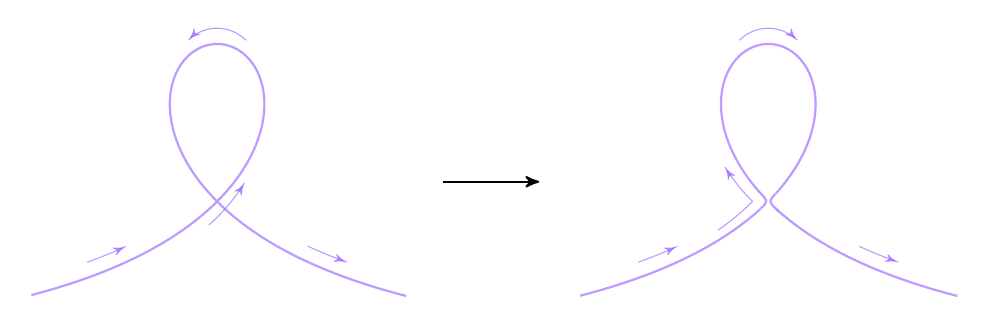
\begin{tikzpicture}[shorten >=1pt,node distance=2cm,on grid,>=stealth',thick,
					every state/.style={fill,draw=none,orange,text=white!80!orange,circular drop shadow},
					accepting/.style ={green!50!black,text=green!50!black!20!white},
					initial/.style ={red,text=white!80!red},scale= 0.25 ]
					\definecolor{qqzzcc}{rgb}{0,0.6,0.8}
					\definecolor{ffdxqq}{rgb}{1,0.84,0}
					\definecolor{zzwwff}{rgb}{0.6,0.4,1}
					\definecolor{ffttww}{rgb}{1,0.2,0.4}
					\definecolor{ffzzzz}{rgb}{1,0.6,0.6}
					\definecolor{ffzztt}{rgb}{1,0.6,0.2}
					
					\draw[color = zzwwff, fill = none,domain=-2:2
  ,samples = 300,opacity = 0.65] plot({8*(\x)*(1-(\x)*(\x))/(1+(\x)*(\x))},{8*(1-(\x)*(\x))/(1+(\x)*(\x))}) ;
				
					\draw[color = zzwwff, fill = none,domain=-1.5:-1.7, thin,  ->
  ,samples = 300,opacity = 0.65] plot({8*(\x)*(1-(\x)*(\x))/(1+(\x)*(\x))},{8*(1-(\x)*(\x))/(1+(\x)*(\x)) +0.8}) ;
					\draw[color = zzwwff, fill = none,domain=1.7:1.5, thin,  ->
  ,samples = 300,opacity = 0.65] plot({8*(\x)*(1-(\x)*(\x))/(1+(\x)*(\x))},{8*(1-(\x)*(\x))/(1+(\x)*(\x)) +0.8}) ;
					\draw[color = zzwwff, fill = none,domain=1.05:0.8, thin,  ->
  ,samples = 300,opacity = 0.65] plot({8*(\x)*(1-(\x)*(\x))/(1+(\x)*(\x))},{8*(1-(\x)*(\x))/(1+(\x)*(\x)) -0.8}) ;
					\draw[color = zzwwff, fill = none,domain=0.2:-0.2, thin,  ->
  ,samples = 300,opacity = 0.65] plot({8*(\x)*(1-(\x)*(\x))/(1+(\x)*(\x))},{8*(1-(\x)*(\x))/(1+(\x)*(\x)) +0.8}) ;
					
					\draw[->,xshift= 14cm] (-2.5,1) -- (2.5,1);

					\begin{scope}[xshift= 28cm]
						\draw[color = zzwwff, fill = none,samples = 300,opacity = 0.65,domain=-2:-1.05]
							plot({8*(\x)*(1-(\x)*(\x))/(1+(\x)*(\x))},{8*(1-(\x)*(\x))/(1+(\x)*(\x))});
						\draw[color = zzwwff, fill = none,samples = 300,opacity = 0.65,domain=0.95:-0.95]
							plot({8*(\x)*(1-(\x)*(\x))/(1+(\x)*(\x))},{8*(1-(\x)*(\x))/(1+(\x)*(\x))});
						\draw[color = zzwwff, fill = none,samples = 300,opacity = 0.65,domain=1.05:2]
							plot({8*(\x)*(1-(\x)*(\x))/(1+(\x)*(\x))},{8*(1-(\x)*(\x))/(1+(\x)*(\x))});
					
						\draw[color = zzwwff, fill = none,samples = 300,opacity = 0.65]
							({8*(-1.06)*(1-(-1.06)*(-1.06))/(1+(-1.06)*(-1.06))},{8*(1-(-1.06)*(-1.06))/(1+(-1.06)*(-1.06))}) .. controls (0,0)
							.. ({8*(0.94)*(1-(0.94)*(0.94))/(1+(0.94)*(0.94))},{8*(1-(0.94)*(0.94))/(1+(0.94)*(0.94))});
						\draw[color = zzwwff, fill = none,samples = 300,opacity = 0.65]
							({8*(-0.94)*(1-(-0.94)*(-0.94))/(1+(-0.94)*(-0.94))},{8*(1-(-0.94)*(-0.94))/(1+(-0.94)*(-0.94))}) .. controls (0,0)
							..({8*(1.06)*(1-(1.06)*(1.06))/(1+(1.06)*(1.06))},{8*(1-(1.06)*(1.06))/(1+(1.06)*(1.06))})   ;
				
				
				
						\draw[color = zzwwff, fill = none,domain=-1.5:-1.7, thin,  ->
  ,samples = 300,opacity = 0.65] plot({8*(\x)*(1-(\x)*(\x))/(1+(\x)*(\x))},{8*(1-(\x)*(\x))/(1+(\x)*(\x)) +0.8}) ;
						\draw[color = zzwwff, fill = none,domain=1.7:1.5, thin,  ->
  ,samples = 300,opacity = 0.65] plot({8*(\x)*(1-(\x)*(\x))/(1+(\x)*(\x))},{8*(1-(\x)*(\x))/(1+(\x)*(\x)) +0.8}) ;
						\draw[color = zzwwff, fill = none,domain=-0.2:0.2, thin,  ->
  ,samples = 300,opacity = 0.65] plot({8*(\x)*(1-(\x)*(\x))/(1+(\x)*(\x))},{8*(1-(\x)*(\x))/(1+(\x)*(\x)) +0.8}) ;
					\draw[color = zzwwff, fill = none,domain=1.2:0.8, thin,  ->
  ,samples = 300,opacity = 0.65] plot({-abs(8*(\x)*(1-(\x)*(\x))/(1+(\x)*(\x))) - 0.8},{8*(1-(\x)*(\x))/(1+(\x)*(\x)) }) ;
					\end{scope}
				\end{tikzpicture}
			\caption{交叉时的转化示意图} \label{12convert}
			\vspace{-1em}
			\end{figure}
			\fi
			
			不妨枚举从哪条边开始访问,然后以要访问的边为轴,依次作出凸多边形的对称图形。那么原问题就转化为,在展开后的图形中,先后经过要被访问的边(虚线),在不出反射后的多边形范围的情况下,回到出发点反射后对应的点,并最小化路线长度。
				\begin{figure}[!htb]	
					\centering
					\definecolor{uuuuuu}{rgb}{0.27,0.27,0.27}
					\definecolor{cczzff}{rgb}{0.8,0.6,1}
					\definecolor{zzwwff}{rgb}{0.6,0.4,1}
					\definecolor{zzttqq}{rgb}{0.6,0.2,0}
					\definecolor{qqqqff}{rgb}{0,0,1}
					\begin{tikzpicture}[line cap=round,line join=round,>=triangle 45,x=1.0cm,y=1.0cm]
						\fill[color=zzttqq,fill=zzttqq,fill opacity=0.1] (2,1) -- (6,1) -- (6,3) -- (3,3) -- cycle;
						\fill[color=zzttqq,fill=zzttqq,fill opacity=0.1] (10,1) -- (6,1) -- (6,3) -- (9,3) -- cycle;
						\fill[color=zzttqq,fill=zzttqq,fill opacity=0.1] (10,5) -- (6,5) -- (6,3) -- (9,3) -- cycle;
						\fill[color=zzttqq,fill=zzttqq,fill opacity=0.1] (10,5) -- (12.4,1.8) -- (10.8,0.6) -- (9,3) -- cycle;
						\fill[color=zzttqq,fill=zzttqq,fill opacity=0.1] (10,5) -- (12.4,1.8) -- (14,3) -- (12.2,5.4) -- cycle;
						\draw [color=zzttqq] (2,1)-- (6,1);
						\draw [dash pattern=on 4pt off 4pt,color=zzttqq] (6,1)-- (6,3);
						\draw [color=zzttqq] (6,3)-- (3,3);
						\draw [color=zzttqq] (3,3)-- (2,1);
						\draw [color=zzttqq] (10,1)-- (6,1);
						\draw [dash pattern=on 4pt off 4pt,color=zzttqq] (6,1)-- (6,3);
						\draw [dash pattern=on 4pt off 4pt,color=zzttqq] (6,3)-- (9,3);
						\draw [color=zzttqq] (9,3)-- (10,1);
						\draw [color=zzttqq] (10,5)-- (6,5);
						\draw [color=zzttqq] (6,5)-- (6,3);
						\draw [dash pattern=on 4pt off 4pt,color=zzttqq] (6,3)-- (9,3);
						\draw [dash pattern=on 4pt off 4pt,color=zzttqq] (9,3)-- (10,5);
						\draw [dash pattern=on 4pt off 4pt,color=zzttqq] (10,5)-- (12.4,1.8);
						\draw [color=zzttqq] (12.4,1.8)-- (10.8,0.6);
						\draw [color=zzttqq] (10.8,0.6)-- (9,3);
						\draw [dash pattern=on 4pt off 4pt,color=zzttqq] (9,3)-- (10,5);
						\draw [dash pattern=on 4pt off 4pt,color=zzttqq] (10,5)-- (12.4,1.8);
						\draw [color=zzttqq] (12.4,1.8)-- (14,3);
						\draw [color=zzttqq] (14,3)-- (12.2,5.4);
						\draw [color=zzttqq] (12.2,5.4)-- (10,5);
						\draw [color=cczzff] (6,2.92)-- (5.7,3);
						\draw [color=cczzff] (3.55,2.26)-- (11.94,4.52);
						\draw [color=cczzff] (7.81,3.41) -- (7.79,3.36);
						\draw [color=cczzff] (7.81,3.41) -- (7.76,3.44);
						\draw [color=cczzff] (7.74,3.39) -- (7.72,3.34);
						\draw [color=cczzff] (7.74,3.39) -- (7.7,3.42);						
						\draw [color=cczzff] (5.79,2.98) -- (5.83,3.01);
\draw [color=cczzff] (5.79,2.98) -- (5.81,2.93);
\draw [color=cczzff] (5.85,2.96) -- (5.9,2.99);
\draw [color=cczzff] (5.85,2.96) -- (5.87,2.91);
\draw [color=cczzff] (5.7,3)-- (2.58,2.16);
\draw [color=cczzff] (4.08,2.56) -- (4.1,2.61);
\draw [color=cczzff] (4.08,2.56) -- (4.12,2.53);
\draw [color=cczzff] (4.14,2.58) -- (4.16,2.63);
\draw [color=cczzff] (4.14,2.58) -- (4.19,2.55);
\draw [color=cczzff] (2.58,2.16)-- (3.04,1);
\draw [color=cczzff] (2.84,1.52) -- (2.78,1.53);
\draw [color=cczzff] (2.84,1.52) -- (2.86,1.56);
\draw [color=cczzff] (2.81,1.58) -- (2.76,1.6);
\draw [color=cczzff] (2.81,1.58) -- (2.84,1.63);
\draw [color=cczzff] (3.04,1)-- (3.55,2.26);
\draw [color=cczzff] (3.32,1.69) -- (3.35,1.65);
\draw [color=cczzff] (3.32,1.69) -- (3.27,1.68);
\draw [color=cczzff] (3.3,1.63) -- (3.32,1.58);
\draw [color=cczzff] (3.3,1.63) -- (3.24,1.61);
\draw [color=cczzff] (3.55,2.26)-- (6,2.92);
\draw [color=cczzff] (4.84,2.61) -- (4.82,2.56);
\draw [color=cczzff] (4.84,2.61) -- (4.8,2.64);
\draw [color=cczzff] (4.77,2.59) -- (4.75,2.54);
\draw [color=cczzff] (4.77,2.59) -- (4.73,2.62);
						\begin{scriptsize}
						\draw[color=cczzff!80!black] ({2-0.11},{1-0.11}) node {$A$};
						\draw[color=cczzff!80!black] ({6-0.11},{1-0.21}) node {$B$};
						\draw[color=cczzff!80!black] ({6-0.21},{3+0.21}) node {$C$};
						\draw[color=cczzff!80!black] ({3-0.11},{3+0.11}) node {$D$};
						\draw[color=cczzff!80!black] ({10+0.11},{1-0.11}) node {$A$};
						\draw[color=cczzff!80!black] ({9-0.21},{3+0.21}) node {$D$};
						\draw[color=cczzff!80!black] ({10},{5+0.21}) node {$A$};
						\draw[color=cczzff!80!black] ({6-0.21},{5+0.21}) node {$B$};
						\draw[color=cczzff!80!black] ({12.4+0.11},{1.8-0.21}) node {$B$};
						\draw[color=cczzff!80!black] ({10.8},{0.6-0.21}) node {$C$};
						\draw[color=cczzff!80!black] ({14+0.21},{3}) node {$C$};
						\draw[color=cczzff!80!black] ({12.2},{5.4+0.21}) node {$D$};
\fill [color=zzwwff](3.55, 2.26) circle (1.5pt);

\draw[color=zzwwff] (3.62,2.48) node {$O$};
\fill [color=zzwwff] (8.45,2.26) circle (1.5pt);
\draw[color=zzwwff] (8.55,2.48) node {$O^\prime$};
\fill [color=zzwwff] (8.45,3.74) circle (1.5pt);
\draw[color=zzwwff] (8.56,3.96) node {$O^{\prime\prime}$};
\fill [color=zzwwff] (9.92,3) circle (1.5pt);
\draw[color=zzwwff] (10.03,3.22) node {$O^{\prime\prime\prime}$};
\fill [color=zzwwff] (11.94,4.52) circle (1.5pt);
\draw[color=zzwwff] (12.04,4.74) node {$O^{(4)}$};
\fill [color=uuuuuu] (6,2.92) circle (1.5pt);
\fill [color=uuuuuu] (5.7,3) circle (1.5pt);
\fill [color=uuuuuu] (2.58,2.16) circle (1.5pt);
\fill [color=uuuuuu] (3.04,1) circle (1.5pt);
\end{scriptsize}
\end{tikzpicture}
			\caption{一个转化的例子} 
			\vspace{-1em}
			\end{figure}
				\newpage
				\begin{wrapfigure}{r}{8cm}
					\centering
\definecolor{cczzff}{rgb}{0.8,0.6,1}
\definecolor{uuuuuu}{rgb}{0.27,0.27,0.27}
\definecolor{ffzzzz}{rgb}{1,0.6,0.6}
\definecolor{zzwwff}{rgb}{0.6,0.4,1}
\definecolor{zzttqq}{rgb}{0.6,0.2,0}
\begin{tikzpicture}[line cap=round,line join=round,>=triangle 45,x=1.0cm,y=1.0cm]
\fill[color=zzttqq,fill=zzttqq,fill opacity=0.1] (2.31,1.22) -- (3.7,1.54) -- (4,3) -- (3,3) -- cycle;
\fill[color=zzttqq,fill=zzttqq,fill opacity=0.1] (4.86,0.7) -- (3.7,1.54) -- (4,3) -- (4.92,2.61) -- cycle;
\fill[color=zzttqq,fill=zzttqq,fill opacity=0.1] (6.25,3.97) -- (4.85,4.23) -- (4,3) -- (4.92,2.61) -- cycle;
\fill[color=zzttqq,fill=zzttqq,fill opacity=0.1] (6.25,3.97) -- (6.54,2.57) -- (5.33,1.7) -- (4.92,2.61) -- cycle;
\fill[color=zzttqq,fill=zzttqq,fill opacity=0.1] (6.25,3.97) -- (6.54,2.57) -- (7.99,2.24) -- (8.01,3.24) -- cycle;
\draw [color=zzttqq] (2.31,1.22)-- (3.7,1.54);
\draw [dash pattern=on 2pt off 2pt,color=zzttqq] (3.7,1.54)-- (4,3);
\draw [color=zzttqq] (4,3)-- (3,3);
\draw [color=zzttqq] (3,3)-- (2.31,1.22);
\draw [color=zzttqq] (4.86,0.7)-- (3.7,1.54);
\draw [dash pattern=on 2pt off 2pt,color=zzttqq] (3.7,1.54)-- (4,3);
\draw [dash pattern=on 2pt off 2pt,color=zzttqq] (4,3)-- (4.92,2.61);
\draw [color=zzttqq] (4.92,2.61)-- (4.86,0.7);
\draw [color=zzttqq] (6.25,3.97)-- (4.85,4.23);
\draw [color=zzttqq] (4.85,4.23)-- (4,3);
\draw [dash pattern=on 2pt off 2pt,color=zzttqq] (4,3)-- (4.92,2.61);
\draw [dash pattern=on 2pt off 2pt,color=zzttqq] (4.92,2.61)-- (6.25,3.97);
\draw [dash pattern=on 2pt off 2pt,color=zzttqq] (6.25,3.97)-- (6.54,2.57);
\draw [color=zzttqq] (6.54,2.57)-- (5.33,1.7);
\draw [color=zzttqq] (5.33,1.7)-- (4.92,2.61);
\draw [dash pattern=on 2pt off 2pt,color=zzttqq] (4.92,2.61)-- (6.25,3.97);
\draw [dash pattern=on 2pt off 2pt,color=zzttqq] (6.25,3.97)-- (6.54,2.57);
\draw [color=zzttqq] (6.54,2.57)-- (7.99,2.24);
\draw [color=zzttqq] (7.99,2.24)-- (8.01,3.24);
\draw [color=zzttqq] (8.01,3.24)-- (6.25,3.97);
\draw [color=ffzzzz] (3.55,2.26)-- (7.26,2.71);
\draw [color=ffzzzz] (5.5,2.5) -- (5.46,2.43);
\draw [color=ffzzzz] (5.5,2.5) -- (5.44,2.55);
\draw [color=ffzzzz] (5.41,2.49) -- (5.37,2.42);
\draw [color=ffzzzz] (5.41,2.49) -- (5.35,2.54);
\draw [color=ffzzzz, ->] (3.86,2.3)-- (3.16,2.7) node[above right,pos=0.5] {\small ?};
\draw [color=cczzff] (3.55,2.26)-- (4.92,2.61);
\draw [color=cczzff] (4.32,2.46) -- (4.29,2.39);
\draw [color=cczzff] (4.32,2.46) -- (4.26,2.5);
\draw [color=cczzff] (4.23,2.43) -- (4.2,2.37);
\draw [color=cczzff] (4.23,2.43) -- (4.18,2.48);
\draw [color=cczzff] (4.92,2.61)-- (7.26,2.71);
\draw [color=cczzff] (6.18,2.66) -- (6.14,2.6);
\draw [color=cczzff] (6.18,2.66) -- (6.13,2.72);
\draw [color=cczzff] (6.09,2.66) -- (6.05,2.6);
\draw [color=cczzff] (6.09,2.66) -- (6.04,2.72);
\begin{scriptsize}
\fill [color=zzwwff] (3.55,2.26) circle (1.5pt);
\draw[color=zzwwff] (3.59,2.39) node {$O$};
\fill [color=zzwwff] (7.26,2.71) circle (1.5pt);
\draw[color=zzwwff] (7.32,2.84) node {$O^{(4)}$};
\fill [color=uuuuuu] (3.86,2.3) circle (1.5pt);
\end{scriptsize}
\end{tikzpicture}
			\caption{直线被遮挡的例子}  \label{12no}
			\vspace{-1em}
			\end{wrapfigure}
			
			显然,如果出发点和其对称点间的线段未经过图外的部分,那么这条线段的长度就是答案;但如果这条线段超出范围了呢?
				
			如图 \ref{12no} ,此时不能直接返回两点间的长度,而应当从多边形结点上稍稍绕远路。具体地,最优的绕法可以通过动态规划求出。设 $F[i]$ 表示从起始点出发反弹若干次后到达 $i$ 点,最短的路线长度。转移
			\begin{align}
				F[i]& =\min_{j, j \text{ 能直接到 } \, i}F[j] + W(j,i)
				\intertext{边界}
				F[i]& = W(\text{出发点} ,i), && \text{出发点能直接到 $i$}\\
				F[i]& = +\infty, && \text{出发点不能直接到 $i$}
			\end{align}
			答案
			\begin{align}
					& \min_{i, i \text{ 能直接到出发点}}F[i]+W(i,\text{出发点})
			\end{align}
			其中 $W(j,i)$ 表示从 $j$  经过中间的边反弹到 $i$且 “走直线” 的长度。
			\subsubsection{时空复杂度}
				时间复杂度 $\mathcal{O}\left(N^3\right)$。
					
				空间复杂度 $\mathcal{O}\left(N^2\right)$。
		\newpage
		\subsection{ACM/ICPC World Finals 2012 I A Safe Bet}
			\subsubsection{题目大意}
				一个 $N \times M$ 的网格里放有 \SI{45}{\degree} 的镜子。问
				\begin{enumerate}
					\item 从第一行左边射入的光能否经过镜子反射,从最后一行右边射出?
					\item 如果 1. 不能实现,那么可否通过在空白格子放一张镜子的方式实现 1.?如果能,在何处(字典序最小)放镜子?
					\item 或者,不放或仅放一张镜子都不能实现 1.?
				\end{enumerate}
				\begin{figure}[!htb]
 					\centering
					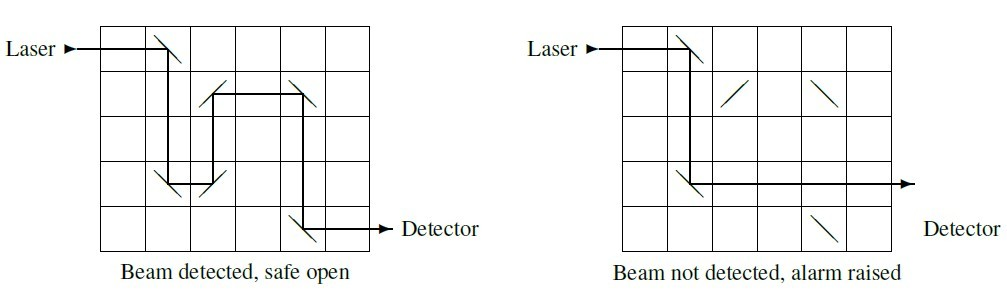
\includegraphics[width=0.8 \textwidth]{4.jpg}
					\caption{两个例子,左图能实现 1.,右图需在 $(4,3) $ 放一张 / 型镜子 才能实现 1.}
				\end{figure}
				
				$N,M \le \num{1 000 000},$ 两种镜子的数量 $p,q$ 分别 $\le \num{200 000}$
			\subsubsection{算法讨论}
				先求出从第一行左端射入的光线轨迹。方法是不断寻找在光线方向上的,且当前离光最近的镜子。具体地,可以先事先对镜子按横坐标优先和纵坐标优先分别排序,这样每行/列相邻的镜子在序列中也会相邻,直接查找当前光线所处镜子在序列中的前(后)一个元素,就是目标镜子。随后按照光线反射定律,计算光线的新方向。若光线射出网格,则退出运算。
					
				如果光线从最后一行向右射出,那么程序返回 1. 是正确的;否则从最后一行右端向左相反地射入光线,并用前述的方法计算其轨迹。只需判断两条轨迹是否有交,并求出交中的最小元素。
					
				求交的过程可转为扫描 $+$ 树状数组。两条轨迹可分为若干横线和若干纵线,那么可分别用一个的横线去交另一个的纵线。具体地,设有一条横向的扫描线从上至下扫描。那么用树状数组维护好扫描线上有哪些纵线。对于横线,则相当于在扫描线上询问区间是否非空。对于第一次非空,求出询问中最小的竖线坐标即可。根据相交的总次数即可回答 2., 3. 问。
			\subsubsection{时空复杂度}
				时间复杂度 $\mathcal{O}\left((p+q)\log(p+q) \right)$。
					
				空间复杂度 $\mathcal{O}\left(p+q\right)$。
		\newpage
		\subsection{ACM/ICPC World Finals 2012 K Stacking Plates}
			\subsubsection{题目大意}
				$N$ 碟盘堆,小盘在大盘上,可能会有相同大小的盘。请使用分割和合并盘子的方式,在保证全过程中小盘在上大盘在下的情况下,将所有盘堆合并为 1 堆。并最小化合并和分割的总次数。
			
				$N \le 50$,各个盘堆的盘子数  $M_i \le 50$。
				
				\begin{figure}[!htb]
 					\centering
					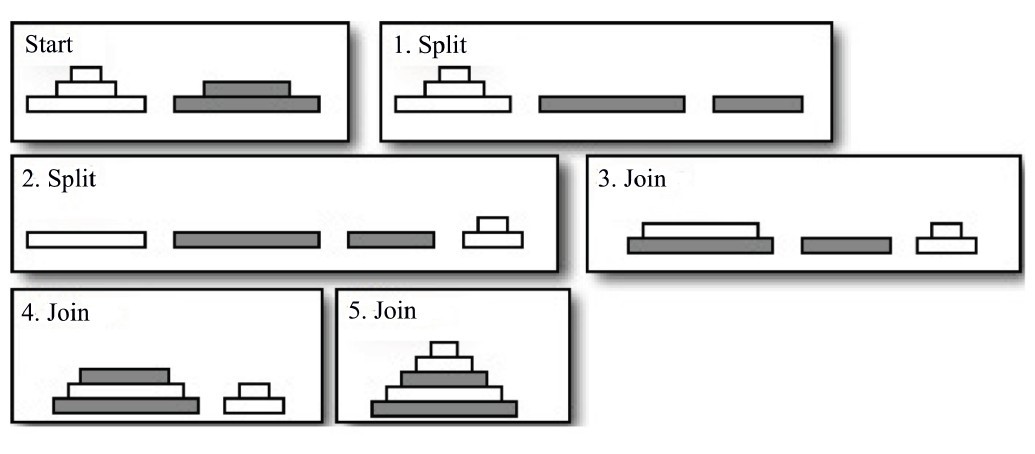
\includegraphics[width=0.8 \textwidth]{5.jpg}
					\caption{样例}
				\end{figure}
				
			\subsubsection{算法讨论}
				为处理方便,先将同一堆中相同大小的盘子合并为一个,并适当修改 $M_i$。显然答案不会被影响,因为可将被合并的看为整体来操作。
				
				由于最后需合并为一个盘堆,故不同大小的盘子的上下顺序就已经确定。只需确定相同大小间盘子的上下顺序,并求出有多少相邻盘子最开始来自于相同盘堆。设这个数为 $x$,那么分析可得答案
				\begin{align}
					Ans = 2 \sum_{i=1}^{N} M_i - N -1 -2x	
				\end{align}
				
				接下来通过动态规划确定最大的 $x$。设 $F[i][j]$ 表示已经确定好大小不超过 $i$ 的盘子的顺序,且其最底部的盘子来自堆 $j$ 的情况下,最大的 $x$。
				\begin{align}
					F[i][j]&= \max_{k} F[Last[i]][k] + [k = j], && \text{大小为  $i$ 的盘子仅存在于盘堆 $j$ }\\
					F[i][j]&= \max_{k} F[Last[i]][k] + \min_{\scriptsize p\ne j,  \atop \text{盘堆  $p$ 有大小为  $i$ 的盘子}}[k = p], && \text{ 大小为  $i$ 的盘子存在于多个盘堆}
				\end{align}边界
				\begin{align}
					F[-\infty][0]&= 0
				\end{align}可求出
				\begin{align} x &= \max_i{F[Last[+\infty]][i]}\end{align}
				其中 $Last[i]$ 表示低于 $i$ 的最大盘子大小。
				
			\subsubsection{时空复杂度}
				时间复杂度 $\mathcal{O}\left(\sum M_iN^3\right)$。使用保存最大值,优先考虑转移的方法,可去掉很多不必要的转移,将时间复杂度优化为 $\mathcal{O}\left(\sum M_iN\right)$。但对本题来说没有必要。
					
				空间复杂度 $\mathcal{O}\left(\sum M_i N\right)$。滚动优化后可降低为 $\mathcal{O}\left(N\right)$。
		\newpage
	
	\section{ACM/ICPC World Finals 2011}
		\subsection{ACM/ICPC World Finals 2011 A To Add or to Multiply}
			\subsubsection{题目大意}
				给定 $a,b,p,q,r,s$。一个程序定义为 对输入的数进行一系列加 $a$ 和乘 $b$ 的操作,并返回最终结果 的操作序列。设计一个程序 $f$,使得任意输入 $x \in [p,q]$,保证输出 $f(x) \in [r,s]$。请先最小化程序的操作总数,再最小化其字典序,并将最优的程序输出。加法 $<$ 乘法。
					
				$a,b,p,q,r,s$ 均为正整数,且 $   \le\num{1e9} $。$p\le q, r\le s$。
			\subsubsection{算法讨论}
				注意到乘法操作是有限的。若 $b=1$,那么乘法操作没有作用,无需执行;否则,设进行了 $multi$ 次乘法操作,那么最大的输出至少为 $q b^{multi}$。要保证输出 $f(x) \le s$ ,就要保证
				\begin{align}
					q b^{multi} &\le s
					\intertext{即}
						 multi& \le \log_b ( s/q)
				\end{align}
				本题中此上限为  $29 (s = \num{1e9},q=1,b=2)$。所以,不妨先枚举 $multi$ 的值。
						
				随后需要考虑加法的操作。设在第 $i$ 次乘法和第 $(i+1)$ 次乘法操作间插入了 $h_{multi-i}$ 次加法操作,特殊地,$h_{multi},h_0$ 分别表示一开始和最后执行的加法操作数。那么对于输入  $x \in [p,q]$,输出
				\begin{align}
					f(x) \in \left[ p b^{multi} + a\Delta ,q b^{multi} + a\Delta \right ] \subset [r,s]
				\end{align}
				其中 $\Delta = \sum_{i=0}^{multi} h_ib^i$。整理得
				\begin{align}
						\frac{r-p b^{multi}}{a} \le \Delta \le \frac{s - q b^{multi} }{a} \label{jiachengzhengli}
				\end{align}
				将 \eqref{jiachengzhengli} 简记为  $u \le \Delta \le v$。那么问题转化为,求一组 $h$,在满足 \eqref{jiachengzhengli} 的情况下,先最小化总和,再最大化 $h$ 的字典序。此问题可以由一个贪心算法解决。从 $h_{multi}$ 起,逐渐增加其值。如果 $\Delta \ge u$,那么构造算法结束;如果将当前的 $h_{\cdot}$ 再增加一会导致  $\Delta > v$,则停止当前位的枚举,转更低位置的 $h_{\cdot}$。这个贪心算法的正确性的证明可以参考进位制。
				\begin{pf}
					设某个 $h$ 的较高位 $h_i$ 本来可以增加一,即 $\sum_{j=0}^{(i-1)} h_jb^j \ge b^i$,那么必然 $ \exists j<i, h_j\ge b$(否则 $\sum_{j=0}^{(i-1)} h_jb^j \le \sum_{j=0}^{(i-1)} (b-1)b^j = b^i -1 < b^i$ 矛盾。)将 $h_j$ 减少 $b$,$h_{(j+1)}$ 增加 $1$。重复以上过程有限次,即可使得 $h_i$ 增加,且 $h$ 的总和在不断减少,新序列会不断地变优,$\Delta$ 也未发生变化。重复寻找新的 $i$ 并且反复更新即可使得任意序列变化为贪心算法给出的解。\qed
				\end{pf}
				显然,上述算法给出的也就是字典序最大的解。
					
				最后,选择各个 $multi$ 值中,答案最优的解输出。 
			\subsubsection{时空复杂度}
				时间复杂度 $\mathcal{O}\left(\log_b^2 ( s/q)\right)$。
					
				空间复杂度 $\mathcal{O}\left(\log_b ( s/q)\right)$。
		\newpage
		\subsection{ACM/ICPC World Finals 2011 B Affine Mess}
			\subsubsection{题目大意}
				给定三个整点构成的点集 $x$。先进行一次未知的旋转变换,再进行未知的伸缩变换和未知的平移变换。已知伸缩变换的系数为非零整数,平移变换的量为整数。旋转变换会使得原来的 $x$ 轴移动到正方形
				$
						D : -10\le x,y\le 10
				$
				的边界的整点上,并把变换后的坐标四舍五入取整。已知 $x$ 经过上述复合变换 $f$ 后变为集合 $y$。试问是否存在 $f$ 以及 $f$ 是否本质相同。本质相同指变换 $ f(\mathbf{x}) = A \mathbf{x} + \mathbf{b}$ 的 $A,\mathbf{b}$ 是唯一的。粗体表示向量。
					
				$x$ 中的坐标的绝对值 $\le 500$,均为整数。
			\subsubsection{算法讨论}
				旋转变换只有 40 种($D$ 边界上,极角 $\in [0,\pi)$ 的整点数)。集合 $x$ 与集合 $y$ 的双射情况只有 $3! = 6$ 种。可先枚举。
				
				随后 $x$ 变换为 $x_0 = \left\{\left(x_1,y_1\right),\left(x_2,y_2\right),\left(x_3,y_3\right)\right\}$。
				设  $y = \left\{\left(X_1,Y_1\right),\left(X_2,Y_2\right),\left(X_3,Y_3\right)\right\}$。问题则变为,是否存在且是否唯一地存在整数 
				$k_x,b_x,k_y,b_y(k_x \ne 0, k_y \ne 0)$ 满足
				\begin{align}
					\begin{cases}
						X_1 = k_x x_1 + b_x\\
						X_2 = k_x x_2 + b_x\\
						X_3 = k_x x_3 + b_x
					\end{cases}
					\text{ 且 } \,\,\,\,\,\,
					\begin{cases}
						Y_1 = k_y y_1 + b_y\\
						Y_2 = k_y y_2 + b_y\\
						Y_3 = k_y y_3 + b_y
					\end{cases}
				\end{align}
				 两个方程组形式类似。以第一个方程组为例,可视为是否存在直线 $y=kx+b, k\ne 0, k\in \mathbb{Z},b \in \mathbb{Z}$ 经过 $(x_1,X_1), (x_2,X_2), (x_3,X_3)$。如果任意两点横坐标相同,纵坐标不同,那么无解($k$ 取无穷大)。如果三点重合,那么整系数整截距的一次函数有无穷多个,返回多解。如果只有两点重合,那么仅能确定一条直线。判断直线的斜率和截距是否为整数,再返回有唯一解或无解。若三点均不重合,那么先判断其是否共线,再判断斜率和截距是否为整数,最后返回唯一解或无解。对第二个方程组也进行相同的操作并合并当前的答案,再累计入总答案之中。
			\subsubsection{时空复杂度}
				时间复杂度 $\mathcal{O}\left(1\right)$。
					
				空间复杂度 $\mathcal{O}\left(1\right)$。
		\newpage
		\subsection{ACM/ICPC World Finals 2011 C Ancient Messages}
			\subsubsection{题目大意}
				给定一个黑白位图,仅包含图
				\ref{11c} 中的符号。各个符号可能会经过拓扑等价处理。请分析各个符号在图中出现的次数。
				\begin{figure}[!htb]
 					\centering
					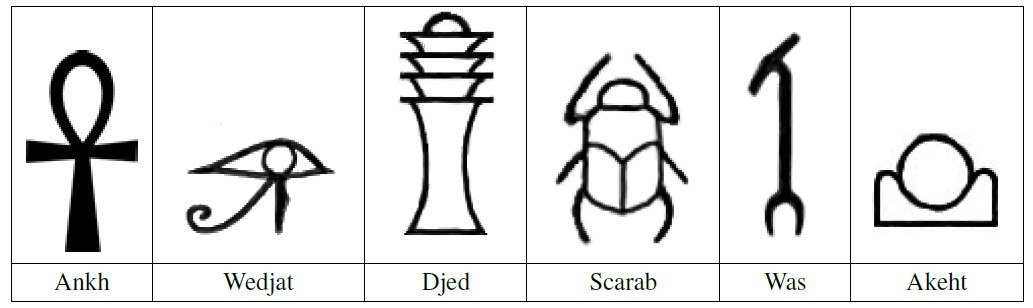
\includegraphics[width=0.8 \textwidth]{6.jpg}
					\caption{位图可能含有的符号}\label{11c}
				
				\end{figure}
				
				位图大小 $N \times M$。$N,M \le 200$。
			\subsubsection{算法讨论}
				经过拓扑等价变换后,图形所含的“空洞”数不会发生变化。恰好,图 \ref{11c} 中的符号的“空洞”数各不相同,可作为辨别它们的依据。
				
				使用 DFS/BFS 算法求出各个极大连通子块所包含的“空洞”数,并与图 \ref{11c} 中个符号的“空洞”数比对,识别之。
			\subsubsection{时空复杂度}
				时间复杂度 $\mathcal{O}\left(NM\right)$。
					
				空间复杂度 $\mathcal{O}\left(NM\right)$。
		\newpage
		\subsection{ACM/ICPC World Finals 2011 E Coffee Central}
			\subsubsection{题目大意}
				矩形 $R: 1\le x \le N, 1 \le y \le M$ 中有若干整点 $(x_i,y_i)$。给定整数 $B$,请另外求一个 $R$ 中的整点 $(x_0,y_0)$,使得原来的整点中满足
				\begin{align}	
					\left|x_i-x_0\right|+\left|y_i-y_0\right| \le B \label{11econstraint}
				\end{align}
				的数量尽可能多。若有多解,先最小化 $y$,再最小化 $x$。 
				
				$N,M \le \num{1000}$。多组测试。一组测试内整点集合是不变的,但有多个待询问的 $B$ 值。
			\subsubsection{算法讨论}
				定义旋转变换 $(x,y) \mapsto (x+y,x-y)$。在此变换下,\eqref{11econstraint} 变为正方形 
				\begin{align}	
					\left\{
						\begin{aligned}
						\left|x_i-x_0\right| & \le B \\
						\left|y_i-y_0\right|& \le B
						\end{aligned}
					\right.
				\end{align}
				那么该正方形内的点数,可以用二维前缀和求出。设 $S[i][j] = \sum_{p\le i \atop q \le j} [(p,q) \text{ 在变换后的点集中}]$。
				\begin{align}	
					S[i][j]=[(i,j) \text{ 在变换后的点集中}] +S[i-1][j]+S[i][j-1]-S[i-1][j-1]
				\end{align}
				对于正方形 $(x_1,y_1) - (x_2,y_2)$,正方形内的点数
				\begin{align}	
					Ans = S[x_2][y_2]-S[x_2][y_1-1]-S[x_1-1][y_2]+S[x_1-1][y_1-1]
				\end{align}
				枚举要选择的点并 $\mathcal{O}(1) $ 计算点数。
			\subsubsection{时空复杂度}
				时间复杂度 $\mathcal{O}\left(NM\right)$。
					
				空间复杂度 $\mathcal{O}\left(NM\right)$。
		\newpage
		\subsection{ACM/ICPC World Finals 2011 F Machine Works}
			\subsubsection{题目大意}
				有 $N$ 个物品。第 $i$ 个物品只能在第 $D_i$ 天买到,价格 $P_i$,回收价 $R_i, P_i > R_i$,回收时间任意,但必须严格在第 $D_i$ 之后。每天只能持有一件物品,
				且从买入第二天起,持有第 $i$ 件物品将会带来 $G_i$ 的收入。过程持续 $D, D_i \le D$ 天,第 $(D+1)$ 天,持有物会被强制回收。
				初期成本 $C$。 求整个过程的最大收益加本金。
			
				$N \le \num{1e5}$。
			\subsubsection{算法讨论}
				构造两个虚拟物品 $i=0,N+1$,分别在第 $0,(D+1)$ 天上市,价格均满足 $P_i,R_i,G_i = 0$。然后,对物品按 $D_i$ 排序。
				
				设 $F[i]$ 表示目前持有物品 $i$ 的收益,则
				\begin{align}
					F[i] &= \max_{j<i} F[j]+(D_i-D_j) \cdot G_j-P_i+R_i
					\intertext{由于最优方案的收益一定随时间单调不降,故只需检测当前本金加利润是否超过 $P_i$,即
					\begin{align}
						F[i]+C-R_i+P_i < P_i
					\end{align}
					若满足上式,则将 $F[i]$ 重置为 $+\infty$。边界
					}
					F[0] &=0
					\intertext{答案}
						Ans &=F[N+1]+C
				\end{align}		
					
				暴力实现耗时 $\mathcal{O}\left(N ^2\right)$。使用斜率优化可降为 $\mathcal{O}\left(N\log N\right)$。
				本题中,斜率单调,但横坐标不单调,故需用数据结构维护凸壳。可以根据斜率删掉之后无用的点,故不需二分最优点。
			\subsubsection{时空复杂度} 
				时间复杂度 $\mathcal{O}\left(N \log N\right)$。
					
				空间复杂度 $\mathcal{O}\left(N\right)$。
		\newpage
		\subsection{ACM/ICPC World Finals 2011 H Mining Your Own Business}
			\subsubsection{题目大意}
				给定无向图 $G=(V,E)$。求点集 $V^\prime \subset V$,使得删去 $G$ 任意一点后,各极大连通分量均存在至少一个点在 $V^\prime$ 中。求最小的 $|V^\prime|$ 以及达到此最小值的方案。
				
				$N = |V| \le \num{5e4}$。
			\subsubsection{算法讨论}
				显然只有割点被删去之后,图的连通性才会发生变化。不妨先求出各个割点。
				
				在原图中删去所有割点,并分别考虑形成的极大连通块。如果该连通块仅与一个割点连接,那么必须在该连通块中选择任意一个结点放入  $V^\prime$  中,方案数为连通块大小。原因是如果此割点被删除,就会违背题目条件。
				
				如果连通块与多个割点连接,那么无需将任何结点放入  $V^\prime$  中,方案数为 1。因为任意割点被断掉后,仍然可通过其他的割点走到属于 $V^\prime$ 的结点。
					
				如果连通块无任何割点连接,那么需放置至少两个结点到 $V^\prime$  中,方案数 $\binom{\text{连通块大小}}{2}$。原因是断掉任意节点虽然无连通性的变化,但至少还要保证一个没有被删掉的结点还在 $V^\prime$ 中。
				
				
			\subsubsection{时空复杂度}
				时间复杂度 $\mathcal{O}\left(N\right)$。
					
				空间复杂度 $\mathcal{O}\left(N\right)$。
		\newpage
		
		\subsection{ACM/ICPC World Finals 2011 I Mummy Madness}
				
				\begin{wrapfigure}{r}{0.35 \textwidth}
					\centering
					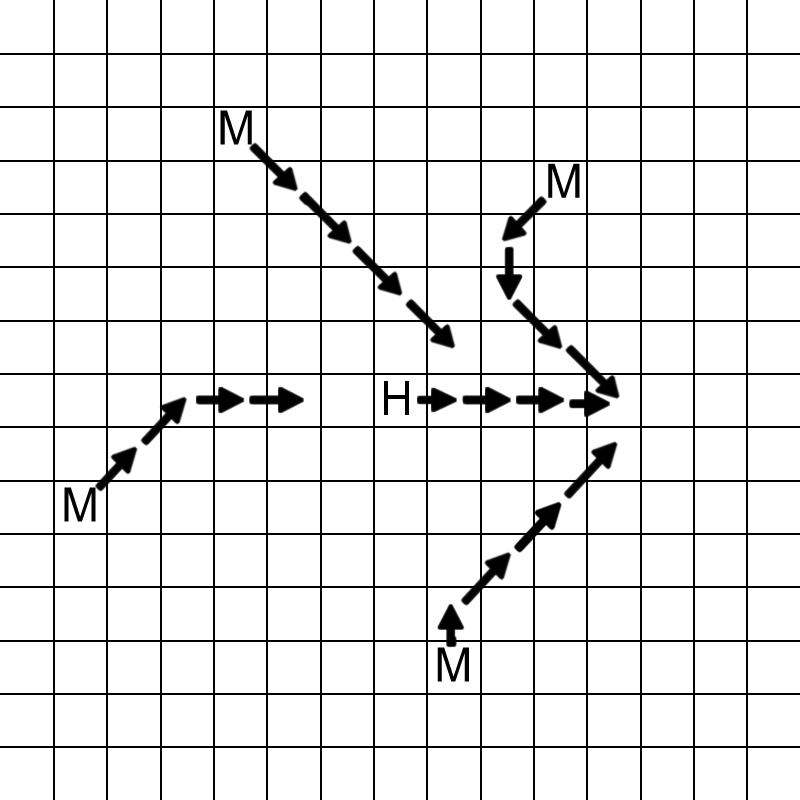
\includegraphics[width=0.3 \textwidth]{5.png}
					\caption{一个可能的局面}
				\end{wrapfigure}
			\subsubsection{题目大意}
				在二维网格中,有一个玩家和 $N$ 个僵尸。玩家每次可以向周围的八个格子移动;随后,\emph{每个}僵尸会\emph{各自}向周围八个格子中,离玩家最近的一个格子移动一步。距离以欧几里德距离计($d = \sqrt{\Delta x^2 + \Delta y^2}$)。一旦僵尸与玩家重合,游戏结束。试问游戏最长能进行多久?
				
				$N \le \num{1e5}$,初始时人和僵尸不重合。
			\subsubsection{算法讨论}
				假定开始时刻 $x = 0$。设 $f(x)$ 表示是否存在一种策略,使得游戏能进行到时刻 $x$。显然 $f(x)$ 关于 $x$ 单调,而答案即使得 $f(x)$ 为真的最大 $x$(可能是 $+ \infty$)。确定答案上界后,不难用二分答案求出答案。
				
				对于特定 $x$,如何求出 $f(x)$ 呢。
				
				记 $R_i$ 表示以第 $i$ 个僵尸为中心,长宽为 $(2 x + 1)$ 且与坐标轴平行的正方形; $R_0$ 表示以人为中心,长宽为 $(2 x + 1)$ 且与坐标轴平行的正方形。
				\begin{theorem}
					直到时刻 $x$,玩家可以躲过所有僵尸当且仅当 $R_0 \setminus (R_1 \cup R_2 \cup \ldots R_N) \ne \varnothing$
				\end{theorem}
				\begin{pf}
					先证充分性。若 $R_0 \setminus (R_1 \cup R_2 \cup \ldots R_N) = A \ne \varnothing$,那么从 $A$ 中任选一个节点 $x$,并\emph{尽早}走向它。
					
					考虑横坐标的投影(纵坐标类似),则玩家需要一路向着 $x$ 行走直到到达 $x$ 后停下。由于
$(R_1 \cup R_2 \cup \ldots R_N)$ 就是所有僵尸在不追玩家的情况下能到达的地方,那么到达 $x$ 后,不管僵尸怎么追,都不会追上主角,故此情况成立。而到达 $x$ 前,对于主角投影点在 $R_i$ 投影区间 中的僵尸 $i$,由于各区间等长,故主角必然向远离 $i$ 的方向运动,在该方向的投影的距离不会变化,故同样追不上主角。综上,必要性成立。
					
					下证必要性。若 $R_0 \setminus (R_1 \cup R_2 \cup \ldots R_N) = \varnothing$,那么不管怎么走,主角都会落入某一个僵尸 $i$ 的 $R_i$ 中。
					
					还是考虑两个方向投影,在主角的投影点与(前文中的)僵尸 $i$ 重合之前,僵尸 $i$ 会一直向着主角的投影方向前进。由于区间等长,如果僵尸 $i$ 的投影从未遇到过主角的投影,那么这个僵尸会走到 $R_i$ 的投影区间中靠近主角的一端;换言之,主角在 $x$ 时不会进入 $R_i$ 的投影区间,与假设矛盾。故总有一刻,其会与主角重合。忽略游戏的停止,假设游戏继续进行,则此僵尸会一直与主角重合。综上,时刻 $x$ 时,僵尸 $i$ 与主角仍会重合,游戏结束,充分性成立。 \qed
				\end{pf}
				根据上述定理,只需用扫描线 + 线段树来确定 $R_0 \setminus (R_1 \cup R_2 \cup \ldots R_N)$ 是否为空即可。具体的,设横坐标为时间轴,纵坐标用线段树维护,那么所有正方形的左边为区间插入事件,右边则为区间删除事件。只需注意是否存在一刻,线段树某个位置上为空。具体的可用打标记的方法实现。有两个标记,一个是此子区间被(完整)覆盖的次数,二是忽略上述的完整覆盖,有多少位置为空。
				
				答案的上限取一个足够大的整数 $U$ 即可。
			\subsubsection{时空复杂度}
				时间复杂度 $\mathcal{O}\left(\log U \cdot(N \log N + N \log U + U)\right)$。使用离散化后,时间复杂度 $\mathcal{O}\left(N \log N\log U\right)$。
					
				空间复杂度 $\mathcal{O}\left(U + N\right)$。
		\newpage
		\subsection{ACM/ICPC World Finals 2011 J Pyramids}
			\subsubsection{题目大意}
				有 $N$ 个木块。搭建一个高度为 $h$ 的\emph{大}金字塔需木块
				\begin{align}
					f(h) & = \sum_{i = 1}^{h} i^2 = (1/6) \cdot  h \cdot (h + 1) \cdot (2 h + 1)
				\intertext{个;搭建一个高度为 $h$ 的\emph{A 型小}金字塔需木块}
					g(h) & = \sum_{i = 1}^{h} {(2i - 1)}^2 = (1/3) \cdot h \cdot (2 h-1) \cdot  (2 h+1)
				\intertext{个;搭建一个高度为 $h$ 的\emph{B 型小}金字塔需木块}
					h(h)  &  = \sum_{i = 1}^{h} {(2i)}^2 = (2/3) \cdot  h \cdot (h + 1) \cdot (2 h + 1)
				\end{align}
				个。要求
				\begin{enumerate}
					\item 用上所有的 $N$ 个木块;
					\item 搭尽量少的金字塔,但必须\emph{超过}一个;
					\item 任意两个金字塔尺寸不同;
					\item 任意金字塔的高度 $h$ \emph{至少为} $2$;
					\item 按金字塔的木块数从大到小排序后,此序列的字典序最大。
				\end{enumerate}
				并输出方案。
				
				$1 \le N \le \num{1e6}$。
				
			\subsubsection{算法讨论}
				枚举可知,满足 $h \ge 2$ 且 $f(h), g(h), h(h) \le N \le \num{1e6}$ 的 $f(h), g(h), h(h)$ 不超过 $a = 321$ 个%,且所需木块数量两两不同
				。
				将其视为物品,进一步使用背包算法求各个大小下最少的物品数可知,任意大小  $1 \le N \le \num{1e6}$,只要存在合法摆法,那么总存在不超过 $b = 6$ 个金字塔的摆法。故在背包算法中,在每一个状态里再辅助计入方案情况,按照题面的信息取最优值即可。
			\subsubsection{时空复杂度}
				时间复杂度 $\mathcal{O}\left(a b N\right)$。
				
				空间复杂度 $\mathcal{O}\left(b N\right)$。$a, b$ 意义同前。
		\newpage
		\subsection{ACM/ICPC World Finals 2011 K Trash Removal}
			\subsubsection{题目大意}
				求\emph{简单}多边形的最小直径。最小直径定义为将多边形旋转某一角度后,多边形内点的纵坐标的最大最小值之差。
				
				多边形顶点数 $n \le \num{100}$。
			\subsubsection{算法讨论}
				一种方法是先求其凸包,再旋转卡壳。
				
				另一种方法是直接对其旋转卡壳。枚举一块木板卡住的两点 $A, B$,枚举另一个木板上可能被卡住的点 $C$。
				那么要求
				\begin{align}
					\forall C, \quad \quad \overrightarrow{AB} \times \overrightarrow{AC} \ge 0 \label{K Trash Removal 1}
				\end{align}
				因为若 \eqref{K Trash Removal 1} 不满足,那么木板就将多边形分成了两半。答案即
				\begin{align}
					Ans = \max_C \frac{ \overrightarrow{AB} \times \overrightarrow{AC}}{ \sqrt{ {\overrightarrow{AB}}^2 }} \label{K Trash Removal 2}
				\end{align}
				因为 \eqref{K Trash Removal 2}  是另一个木板应存在的位置。
				此处叉积定义为空间叉积在 $z$ 轴的投影,即
				\begin{align}
					(x_1, y_1) \times(x_2, y_2) = \begin{vmatrix} x_1 & y_1 \\ x_2 & y_2 \\\end{vmatrix}
				\end{align}
				
				有一些常数优化,例如枚举了 $\overrightarrow{AB}$ 就不必再枚举 $\overrightarrow{BA}$,而只需在枚举 $\overrightarrow{AB}$ 时将计算出的值取反等等。
			\subsubsection{时空复杂度}
				先求其凸包,再旋转卡壳:时间复杂度  $\mathcal{O}\left(N\right)$。
				
				直接旋转卡壳:时间复杂度  $\mathcal{O}\left(N^3\right)$。
				
				空间复杂度 $\mathcal{O}\left(N\right)$。
				
				
		\newpage
				
	
	\section{ACM/ICPC World Finals 2010}
		\subsection{ACM/ICPC World Finals 2010 B Barcodes}
			\subsubsection{题目大意}
				条形码能对 0 到 9,横杠 – 编码。如下表
				\begin{table}[!htb]
					\centering
					\begin{tabular}{ccccccccccc}
						\toprule
							符号 & 编码&&符号 & 编码 && 符号 & 编码&&符号 & 编码   \\
						\midrule
							0 & 00001 && 3 & 11000 && 6 & 01100 & & 9 & 10000 \\
							1 & 10001 && 4 & 00101 && 7 & 00011 && – & 00100 \\
							2 & 01001 && 5 & 10100 && 8 & 10010 && 起/止 & 00110 \\
						\bottomrule
					\end{tabular}
					\caption{编码}
				\end{table}
				
				其中 0 表示细线,1 表示粗线,是 0 粗细的\emph{两倍},颜色交替出现。最后还有两位校验码,计算方法在题面中已给出,并且首尾还需加上起止码。输入扫描器识别到的线的粗细,并容忍 $5 \%$ 的长度误差,请尝试识别信息,并返回返回正确的解码信息,或告知系统校验码错误,或根本无法识别。
				
				线段的条数 $N \le 150$。$1 \le $ 粗细 $ \le 200$。

			\subsubsection{算法讨论}
				如果已经识别出来孰粗孰细,那么接下来就确认方向。由于起止码不对称,故方向是很好确定的。随后按照编码解码,计算校验码,并返回结果即可。下述如何识别粗细。
				
				一个正确的条形码中粗的和细的条纹都出现过(至少起止码里就有)。那么最粗的长度 $Max$ 肯定是 1,最细的 $Min$ 肯定是 0。设 0 的参考粗细为 $a$,那么
				\begin{align}
					x \text{ 表示细条}, \quad \quad & \frac{19}{20} \, a \le x \le \frac{21}{20} \,  a\\
					x \text{ 表示粗条}, \quad \quad & \frac{38}{20} \,  a \le x \le \frac{42}{20} \,  a
				\end{align}
				可以导出
				\begin{align}
					&&  \frac{20}{21} \,  Min &\le a \le \frac{20}{19} \,  Min\\
					x \text{ 表示细条},&&\quad \quad  \frac{20}{21} \, x& \le a \le \frac{20}{19} \,  x \label{B Barcodes 3} \\
					x \text{ 表示粗条},&&\quad \quad  \frac{20}{42} \, x& \le a \le \frac{20}{38} \,  x \label{B Barcodes 4} \\
				\intertext{以及}
					x \text{ 表示细条},&&\quad \quad  \frac{19}{21} \, Min &\le x \le \frac{21}{19} \,  Min \label{B Barcodes 1}\\
					x \text{ 表示粗条},&& \quad \quad  \frac{38}{21} \, Min &\le x \le \frac{42}{19} \,  Min \label{B Barcodes 2}
				\end{align}
				由于 $21 / 19 < 38 / 21$,故可以依据 \eqref{B Barcodes 1} \eqref{B Barcodes 2} 准确识别出粗细。但是即使所有线条粗细都落在  \eqref{B Barcodes 1} \eqref{B Barcodes 2} 中,也并不意味着能够找到一个满足如此要求的 $a$。但根据  \eqref{B Barcodes 3} \eqref{B Barcodes 4},只要 
				\begin{align}
						\max {\left( \max_{\text{细} x} \frac{20}{21} \, x,  \max_{\text{粗} x} \frac{20}{42} \, x \right)} \le
						\min {\left( \min_{\text{细} x} \frac{20}{19} \, x,  \min_{\text{粗} x} \frac{20}{38} \, x \right)}
				\end{align}
				满足,就能找到一个中间的 $a$;否则应仍然返回无解。
				
			\subsubsection{时空复杂度}
				时间复杂度 $\mathcal{O}\left(N\right)$。
					
				空间复杂度 $\mathcal{O}\left(N\right)$。
		\newpage
		\subsection{ACM/ICPC World Finals 2010 C Tracking Bio-bots}
			\subsubsection{题目大意}
				一个 $N \times M$ 的网格有 $K$ 个高为 1 长度若干的墙。一辆车只能往上和右行走,且不能跨墙。问有多少起始位置可使的汽车能够到达右上角。
				\begin{figure}[!htb]
					\centering
					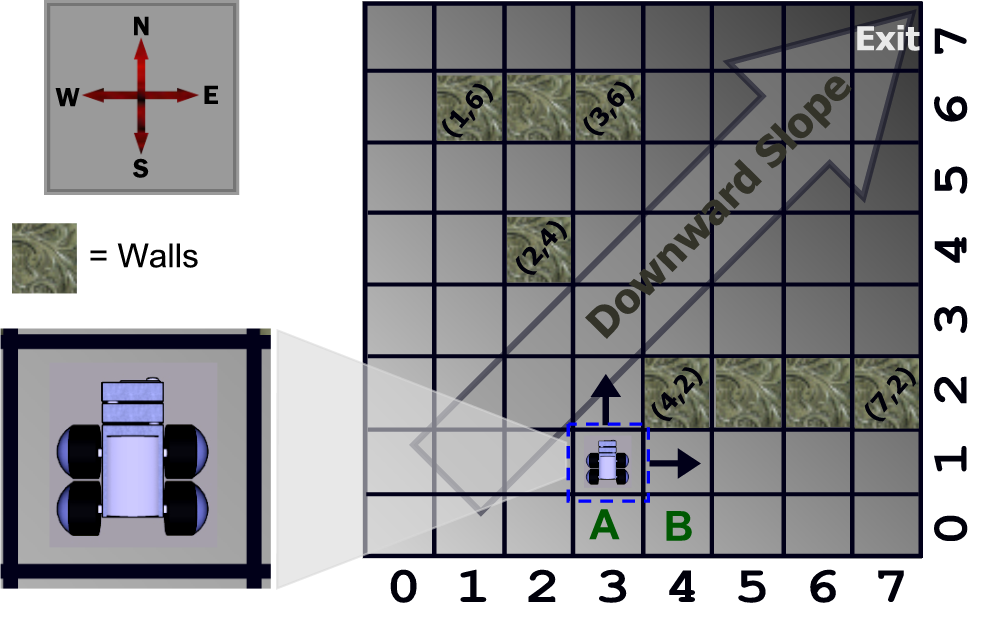
\includegraphics[width=0.75 \textwidth]{6.png}
					\caption{一个可能的局面}
				\end{figure}
				
				$N, M \le \num{1e6}, K \le \num{1e3}$。

			\subsubsection{算法讨论}
				可以得出一个 时间复杂度 $\mathcal{O}\left(N \times M\right)$ 的动态规划。
				\begin{align}
					F[1][M] & = \text{真}\\
					F[i][j] & = (F[i - 1][j] \lor F[i][j + 1]) \land (i, j) \text{ 不是墙}\\
					Ans & = \sum_{F[i][j]\text{ 为真}} 1
				\end{align}
				注意到只有最多 \num{1e3} 堵墙,故将整个平面离散化后,$N, M$ 都会变为  $\mathcal{O}\left(K\right)$ 的,这样这个动态规划就可以在有限的时间内出解了。
			\subsubsection{时空复杂度}
				时间复杂度 $\mathcal{O}\left(K^2\right)$。
					
				空间复杂度 $\mathcal{O}\left(K^2\right)$。
		\newpage
		\subsection{ACM/ICPC World Finals 2010 D Castles}
			\subsubsection{题目大意}
				一个树 $T = (V, E)$,点有三个权 $W_{1, 2, 3}: V \mapsto \mathbb{R}_{+}$。 若干人一起在树上行走,如果走到一个从未访问的点 $x \in V$,那么\emph{必须}访问该节点,并要求此时至少有 $W_1(x)$ 个人,同时会有 $W_2(x)$ 个人死去(并且要求到达时至少有这么多人),并且还要  $W_3(x)$  个人留在这里(人也要够),脱离大部队。访问完所有节点,且所有边两个方向至多走一次。问开始时至少
				要有多少人才能完成任务?起点任意。
				
				点数 $N = |V| \le 100$。
			\subsubsection{算法讨论}
				注意到死去的人和留下的人本质实质上是相同的,都不能帮助拼凑接下来游行的人数,故将其先合并 $\forall x \in V, W_0(x) = W_2(x) + W_3(x)$。
				
				由于所有边两个方向至多走一次,那么旅行的本质实质上是,先从某一节点起访问,然后顺次完整地访问其各个儿子的子树,最后回到此节点%及父节点
				。
				故不妨先枚举起点(即根节点),令 $F[x]$ 表示遍历根为  $x$  的子树至少需要多少人,$G[x]$ 表示遍历根为  $x$  的子树会死(留下)多少人。后者容易求出
				\begin{align}
					G[x] = W_0(x) + \sum_{x\text{ 的儿子}\, y}  G[y]
				\end{align}
				而前者需要求出一个最优的访问儿子的顺序。
				
				不妨假设先求出了以儿子为根的子树的 $F[\cdot], G[\cdot]$,并且得到了一个访问儿子的顺序 $p_1, p_2, ..., p_k$,那么一开始的人数 $x$ 满足
				\begin{align}
					\left\{\setlength{\tabcolsep}{2.5pt}
						\begin{tabular}{rcl}
							$x$ & $\ge$& $W_1(x)$\\
							$x - W_0(x)$ & $\ge$& $ F[p_1]$\\
							$x - W_0(x) - G[p_1]$ & $\ge$& $ F[p_2]$\\
							$x - W_0(x) - G[p_1] - G[p_2]$ & $\ge$& $ F[p_3]$\\
							&  $\cdots$ &  \\
							$x - W_0(x) - G[p_1] - \cdots - G[p_{k-1}]$ & $\ge$&$ F[p_k]$\\
							$x - W_0(x) - G[p_1] - \cdots - G[p_{k}]$ & $\ge$&$ 0$\\
						\end{tabular}\label{D Castles}
					\right.
				\end{align}
				考虑中间的两个相邻方程 $(0 \le i \le k - 2)$
				\begin{align}
							x - W_0(x) - G[p_1] - \cdots - G[p_i] & \ge F[p_{i + 1}]\\
							x - W_0(x) - G[p_1] - \cdots - G[p_{i + 1}] & \ge F[p_{i + 2}]
				\intertext{即}
							x - W_0(x) - G[p_1] - \cdots - G[p_i] & \ge F[p_{i + 1}] \label{DCastlesA} \\
							x - W_0(x) - G[p_1] - \cdots - G[p_i] & \ge G[p_{i + 1}] + F[p_{i + 2}] \label{DCastlesB}
				\end{align}
				如果 $G[p_{i + 1}] - F[p_{i + 1}] \ge G[p_{i + 2}] - F[p_{i + 2}] $ 那么
				\begin{align}
							F[p_{i+2}] \le G[p_{i + 1}] + F[p_{i + 2}] \ge F[p_{i + 1}] + G[p_{i + 2}] \ge F[p_{i + 1}]
				\end{align}
				并交换 $p_{i + 1}, p_{i + 2}$,\label{D Castles A} \label{D Castles B} 变为
				\begin{align}
							x - W_0(x) - G[p_1] - \cdots - G[p_i] & \ge F[p_{i + 2}] \label{DCastlesC}\\
							x - W_0(x) - G[p_1] - \cdots - G[p_i] & \ge G[p_{i + 2}] + F[p_{i + 1}]\label{DCastlesD}
				\end{align}
				\eqref{DCastlesC}  相对于 \eqref{DCastlesB},\eqref{DCastlesD} 相对于 \eqref{DCastlesA} 都更松了,故 $x$ 的解集更大了。
				重复上述过程,直到 $p_i$ 按照  $G[p_{i}] - F[p_{i}]$ 排序,此时  $x$ 的解集最大,且能取到最小值。又因初始序列具有任意性,故此解即为最小解。
				
				故直接排序确定顺序,后参考 \eqref{D Castles} 即可确定 $F[\cdot]$ 的值。最终答案为 $F[\text{根节点}]$ 的最小值。 
			
			\subsubsection{时空复杂度}
				时间复杂度 $\mathcal{O}\left(N^2\log N \right)$。
					
				空间复杂度 $\mathcal{O}\left(N\right)$。
		\newpage
		\subsection{ACM/ICPC World Finals 2010 F Contour Mapping}
				
				\begin{wrapfigure}{r}{0.45 \textwidth}
					\centering
					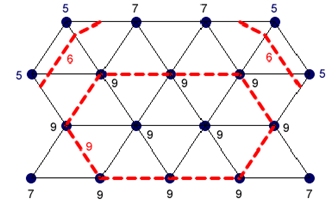
\includegraphics[width=0.4 \textwidth]{7.png}
					\caption{等高线} \vskip-2.5em
				\end{wrapfigure}
			\subsubsection{题目大意}
				如右图的地图,每个实心点都有一个高度,各三角形在空间中过对应点。等高线表示海拔为某高度 $h$ 的整数倍,图形的\emph{轮廓}。求等高线长度。
				
				图形有 $N$ 行,奇数行有 $M$ 列。$N, M \le \num{100}$。$1 \le h \le \num{1000}$,海拔 $\le \num{1e6}$。
			\subsubsection{算法讨论}
				先考虑不过三角形的边界的等高线。由于这一部分等高线就是平面 $z = kh$ 与三角形平面交出的直线,故过三角形的边上的两点。求出三角形边上海拔为 $kh, k \in N^+$ 的点,并将其对应地连接。计算可知同一个三角形内相邻线段长度为等差数列,使用公式求和便知。
					
				对于在三角形边界上的等高线,先需枚举相邻,等高的两点,并判断以其为边界的两个三角形的对点的高度也是均和此边线否一致(须位于图形内)——如果是,那么这条边界不是等高线;反之,是等高线,计入答案。
					
				求和便知。
			\subsubsection{时空复杂度}
				时间复杂度 $\mathcal{O}\left(N \times M \right)$。
				
				空间复杂度 $\mathcal{O}\left(N \times M \right)$。
		\newpage
		\subsection{ACM/ICPC World Finals 2010 J Sharing Chocolate}
			\subsubsection{题目大意}
				有一个 $N \times M$ 网格。你需要用剪刀,每次沿着网格,不拐弯,一刀将其剪成两部分。操作可重复若干次,但最终必切成 $K$ 块,且 $K$ 块的大小须为指定的大小(格子数而非长宽)。问是否有一个可行的操作方案。
				
				$N, M \le 100, K \le 15$。
			\subsubsection{算法讨论}
				动态规划。设 $F[N][S]$ 表示当前需要剪出可重集 $S$ 里的块数,且现在网格长 $N$ 宽 $\sum_{i \in S} i / N$ 的情况下,是否有可行的方案。
				\begin{align}
					F[N][S] &= \text{真}, & |S| = 1\\
					F[N][S] &= \LOR_{\text{枚举裁剪方法,且} \atop \text{剪出一块 $x \in S$}} { F[\text{新尺寸的长度}][S \setminus\{ x\}] }
				\end{align}
				% 此处的求和 $(\sum)$ 表示逻辑析取$(\lor)$。
				
				答案即 $F[N][\text{指定的大小}]$。
			\subsubsection{时空复杂度}
				时间复杂度 $\mathcal{O}\left(N^2 2^K \right)$。
				
				空间复杂度 $\mathcal{O}\left(N 2^K \right)$。
		\newpage
		\subsection{ACM/ICPC World Finals 2010 K Paperweight}
			\subsubsection{题目大意}
给定三维空间中一个有五个顶点的多面体,内部有一个固定点 $A$。请将其放在桌面上,使得即使重心微移了 $\mathbf{\epsilon}, \epsilon \le 0.2$ 后,也仍然稳定(合力矩 $ = \mathbf{0}$),求所有放法中,固定点 $A$ 离桌面的最近和最远距离。

			\subsubsection{算法讨论}
				不妨枚举底面。根据物理知识,力矩平衡当且仅当重心在桌面的投影在支撑面(多面体与桌面接触的面)内。考虑微移 $\mathbf{\epsilon}, \epsilon \le 0.2$,等价于支撑面各边向内平移$ \epsilon$ 单位,方向垂直于边界。直接使用这个进行判断放法的合法性。
				
				枚举底面后,需要计算点面距离。设该面上三个不公线的点 $P, Q, R$,则法向量 $\mathbf{v} = \overrightarrow{PQ} \times  \overrightarrow{PR}$,点面距
				\begin{align}
					\pm d & = \frac{\overrightarrow{AP} \cdot \mathbf{n}}{n} =  \frac{\overrightarrow{AP} \cdot \mathbf{n}}{\sqrt{ {\mathbf{n}}^2 }}  = \frac{\overrightarrow{AP} \cdot \left(\overrightarrow{PQ} \times  \overrightarrow{PR}\right)}{\sqrt{ {\left(\overrightarrow{PQ} \times  \overrightarrow{PR}\right)}^2 }}
				\end{align}
				取 $d$ 的最大最小值即可。
				
				特殊处理退化成四面体的图形(若视为五面体,则有两面都是底面)。
			\subsubsection{时空复杂度}
				时间复杂度 $\mathcal{O}\left(1 \right)$。
				
				空间复杂度 $\mathcal{O}\left(1 \right)$。
		\newpage
	
	\section{ACM/ICPC World Finals 2009}
		\subsection{ACM/ICPC World Finals 2009 B My Bad}
				\begin{wrapfigure}{r}{0.35 \textwidth}
					\centering
					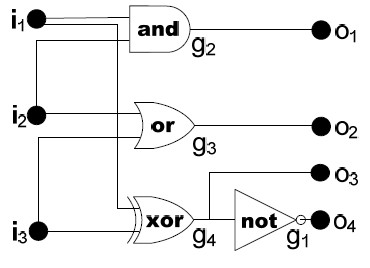
\includegraphics[width=0.3 \textwidth]{7.jpg}
					\caption{一个可能的门电路}
				\end{wrapfigure}
			\subsubsection{题目大意}
				给定一个门电路和若干次实验数据(输入,输出),判断是否
				\begin{enumerate}
					\item 全部元件工作正常;
					\item 某一个元件一直输出一,其他元件正常;
					\item 某一个元件一直输出零,其他元件正常;
					\item 某一个元件一直输出的值与正确的值相反,其他元件正常;或
					\item 有多种可能的故障,或只可能是多个元件的故障,或一个元件的多种故障,或无法判定其故障。
				\end{enumerate}
				
				门电路的数量 $N \le 19$,输入 $M \le 8$,输出 $K \le 19$。不同测试的输入两两不同。
			\subsubsection{算法讨论}
				直接枚举前四种情况,总共有 $(3 N + 1)$ 种可能(全部工作正常,某一元件有某一故障)。测试数最多 $2^M$ 种,代入  $(3 N + 1)$ 种可能中依次检验。若\emph{只有}某一种可能符合要求,那么答案就是该种可能;否则答案为最后一种情况。
				
				模拟逻辑电路时,需先拓扑排序,再计算。
			\subsubsection{时空复杂度}
				
				时间复杂度 $\mathcal{O}\left(N2^MN\right)$。
					
				空间复杂度 $\mathcal{O}\left(N 2^M(M + N)\right)$。
		\newpage
		\subsection{ACM/ICPC World Finals 2009 C The Return of Carl}
				\begin{wrapfigure}{r}{0.35 \textwidth}
					\centering
					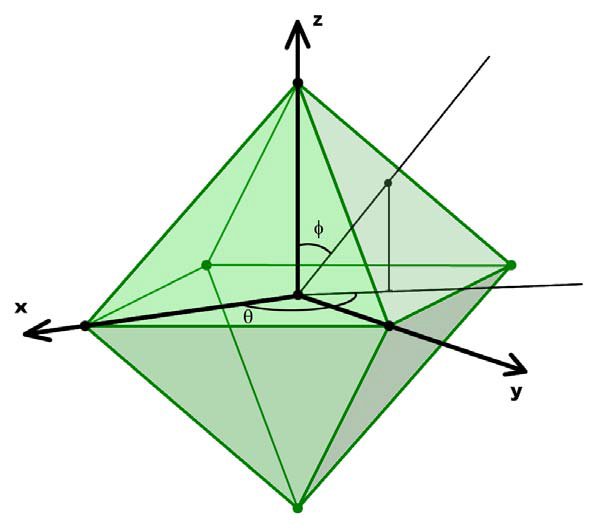
\includegraphics[width=0.3 \textwidth]{8.png}
					\caption{题目中的球坐标系}\label{09c1}
					\vskip-5em
				\end{wrapfigure}
			\subsubsection{题目大意}
				一个正八面体表面上有两点,问从一点经表面到达另一点的最短距离。
				
				坐标使用如图 \ref{09c1} 的球坐标系描述。
			\subsubsection{算法讨论}
				根据正八面体的对称性,可以将某一点旋转,翻转到第一卦限$(x, y, z > 0)$。根据另一个点的卦限分情况讨论。
				
				若另一点位于
				
				\begin{description}
					\item[第一卦限, \Rmnum{1}, $(+, +, +)$] 显然就是两点间的直线距离。
					\item[第二卦限, \Rmnum{2}, $(-, +, +)$] 将八面体一二卦限的面展开为平面,可以证明(暴力搜索)展开后两点的距离就是答案。
					\item[第三卦限, \Rmnum{3}, $(-, -, +)$] 将八面体一二三四卦限的面展开为平面,注意此处两个 \Rmnum{3} 的位置都有可能成为答案,同样可以证明展开后两点的距离就是答案。
					\item[第四卦限, \Rmnum{4}, $(+, -, +)$] 类似 第二卦限, \Rmnum{2}, $(-, +, +)$。
					\item[第五卦限, \Rmnum{5}, $(+, +, -)$] 类似 第二卦限, \Rmnum{2}, $(-, +, +)$。
					\item[第六卦限, \Rmnum{6}, $(-, +, -)$] 类似 第三卦限, \Rmnum{3}, $(-, -, +)$,有两个可能成为答案的位置。
				\begin{figure}[htb]
				\centering
				\definecolor{ffccww}{rgb}{1,0.8,0.4}
\begin{tikzpicture}[line cap=round,line join=round,>=triangle 45,x=1.0cm,y=1.0cm]
\fill[color=ffccww,fill=ffccww,fill opacity=0.25] (0,1.73) -- (1,0) -- (-1,0) -- cycle;
\node[color=ffccww] at (0, 1.73/3) {\Rmnum{1}};
\node[color=ffccww] at (1, 2 * 1.73/3) {\Rmnum{2}};
\node[color=ffccww] at (- 1, 2 * 1.73/3) {\Rmnum{4}};
\node[color=ffccww] at (1, 4 * 1.73/3) {\Rmnum{3}};
\node[color=ffccww] at (- 1, 4 * 1.73/3) {\Rmnum{3}};
\node[color=ffccww] at (2, 5 * 1.73/3) {\Rmnum{7}};
\node[color=ffccww] at (- 2, 5 * 1.73/3) {\Rmnum{7}};
\node[color=ffccww] at (2, 1.73/3) {\Rmnum{6}};
\node[color=ffccww] at (-2, 1.73/3) {\Rmnum{8}};
\node[color=ffccww] at (3, 2 * 1.73/3) {\Rmnum{7}};
\node[color=ffccww] at (- 3, 2 * 1.73/3) {\Rmnum{7}};
\node[color=ffccww] at (- 0, - 1  * 1.73/3) {\Rmnum{5}};
\node[color=ffccww] at (1, - 2  * 1.73/3) {\Rmnum{6}};
\node[color=ffccww] at (- 1, - 2  * 1.73/3) {\Rmnum{8}};
\node[color=ffccww] at (1, - 4  * 1.73/3) {\Rmnum{7}};
\node[color=ffccww] at (- 1, - 4  * 1.73/3) {\Rmnum{7}};
\fill[color=ffccww,fill=ffccww,fill opacity=0.25] (0,1.73) -- (-2,1.73) -- (-1,0) -- cycle;
\fill[color=ffccww,fill=ffccww,fill opacity=0.25] (0,1.73) -- (1,0) -- (2,1.73) -- cycle;
\fill[color=ffccww,fill=ffccww,fill opacity=0.25] (-3,0) -- (-2,1.73) -- (-1,0) -- cycle;
\fill[color=ffccww,fill=ffccww,fill opacity=0.25] (3,0) -- (1,0) -- (2,1.73) -- cycle;
\fill[color=ffccww,fill=ffccww,fill opacity=0.25] (-3,0) -- (-2,1.73) -- (-4,1.73) -- cycle;
\fill[color=ffccww,fill=ffccww,fill opacity=0.25] (3,0) -- (4,1.73) -- (2,1.73) -- cycle;
\fill[color=ffccww,fill=ffccww,fill opacity=0.25] (0,1.73) -- (-2,1.73) -- (-1,3.46) -- cycle;
\fill[color=ffccww,fill=ffccww,fill opacity=0.25] (-3,3.46) -- (-2,1.73) -- (-1,3.46) -- cycle;
\fill[color=ffccww,fill=ffccww,fill opacity=0.25] (0,1.73) -- (1,3.46) -- (2,1.73) -- cycle;
\fill[color=ffccww,fill=ffccww,fill opacity=0.25] (3,3.46) -- (1,3.46) -- (2,1.73) -- cycle;
\fill[color=ffccww,fill=ffccww,fill opacity=0.25] (0,-1.73) -- (1,0) -- (-1,0) -- cycle;
\fill[color=ffccww,fill=ffccww,fill opacity=0.25] (0,-1.73) -- (-2,-1.73) -- (-1,0) -- cycle;
\fill[color=ffccww,fill=ffccww,fill opacity=0.25] (0,-1.73) -- (-2,-1.73) -- (-1,-3.46) -- cycle;
\fill[color=ffccww,fill=ffccww,fill opacity=0.25] (0,-1.73) -- (1,0) -- (2,-1.73) -- cycle;
\fill[color=ffccww,fill=ffccww,fill opacity=0.25] (0,-1.73) -- (1,-3.46) -- (2,-1.73) -- cycle;
\draw [color=ffccww] (0,1.73)-- (1,0);
\draw [color=ffccww] (1,0)-- (-1,0);
\draw [color=ffccww] (-1,0)-- (0,1.73);
\draw [color=ffccww] (0,1.73)-- (-2,1.73);
\draw [color=ffccww] (-2,1.73)-- (-1,0);
\draw [color=ffccww] (-1,0)-- (0,1.73);
\draw [color=ffccww] (0,1.73)-- (1,0);
\draw [color=ffccww] (1,0)-- (2,1.73);
\draw [color=ffccww] (2,1.73)-- (0,1.73);
\draw [color=ffccww] (-3,0)-- (-2,1.73);
\draw [color=ffccww] (-2,1.73)-- (-1,0);
\draw [color=ffccww] (-1,0)-- (-3,0);
\draw [color=ffccww] (3,0)-- (1,0);
\draw [color=ffccww] (1,0)-- (2,1.73);
\draw [color=ffccww] (2,1.73)-- (3,0);
\draw [color=ffccww] (-3,0)-- (-2,1.73);
\draw [color=ffccww] (-2,1.73)-- (-4,1.73);
\draw [color=ffccww] (-4,1.73)-- (-3,0);
\draw [color=ffccww] (3,0)-- (4,1.73);
\draw [color=ffccww] (4,1.73)-- (2,1.73);
\draw [color=ffccww] (2,1.73)-- (3,0);
\draw [color=ffccww] (0,1.73)-- (-2,1.73);
\draw [color=ffccww] (-2,1.73)-- (-1,3.46);
\draw [color=ffccww] (-1,3.46)-- (0,1.73);
\draw [color=ffccww] (-3,3.46)-- (-2,1.73);
\draw [color=ffccww] (-2,1.73)-- (-1,3.46);
\draw [color=ffccww] (-1,3.46)-- (-3,3.46);
\draw [color=ffccww] (0,1.73)-- (1,3.46);
\draw [color=ffccww] (1,3.46)-- (2,1.73);
\draw [color=ffccww] (2,1.73)-- (0,1.73);
\draw [color=ffccww] (3,3.46)-- (1,3.46);
\draw [color=ffccww] (1,3.46)-- (2,1.73);
\draw [color=ffccww] (2,1.73)-- (3,3.46);
\draw [color=ffccww] (0,-1.73)-- (1,0);
\draw [color=ffccww] (1,0)-- (-1,0);
\draw [color=ffccww] (-1,0)-- (0,-1.73);
\draw [color=ffccww] (0,-1.73)-- (-2,-1.73);
\draw [color=ffccww] (-2,-1.73)-- (-1,0);
\draw [color=ffccww] (-1,0)-- (0,-1.73);
\draw [color=ffccww] (0,-1.73)-- (-2,-1.73);
\draw [color=ffccww] (-2,-1.73)-- (-1,-3.46);
\draw [color=ffccww] (-1,-3.46)-- (0,-1.73);
\draw [color=ffccww] (0,-1.73)-- (1,0);
\draw [color=ffccww] (1,0)-- (2,-1.73);
\draw [color=ffccww] (2,-1.73)-- (0,-1.73);
\draw [color=ffccww] (0,-1.73)-- (1,-3.46);
\draw [color=ffccww] (1,-3.46)-- (2,-1.73);
\draw [color=ffccww] (2,-1.73)-- (0,-1.73);
\end{tikzpicture}
				\caption{正八面体的展开图}\label{09c2}
				\end{figure}

					\item[第七卦限, \Rmnum{7}, $(-, -, -)$] 最复杂的一种情况,需要将整个多面体都展开。总共有六个可能的位置,如图  \ref{09c2}。
					\item[第八卦限, \Rmnum{8}, $(+, -, -)$] 类似 第三卦限, \Rmnum{3}, $(-, -, +)$,有两个可能成为答案的位置。
				
				\end{description}
				
				
				至于计算极坐标对应的点在展开图上的位置,可以先计算其在三维坐标系中的位置,方法是解方程

				\begin{align}
					\left\{\begin{array}{rcl}
							x &= &r \sin\theta \cos\phi \\
							y &  =&r \sin\theta \sin\phi \\
							z & =& r \cos\theta\\
							|x| + |y| + |z| & =&  1
						\end{array}
					\right.
				\end{align}
				随后确定其所在平面在展开图的\emph{线性}映射关系,从而计算出我们需要的值。
			\subsubsection{时空复杂度}
				
				时间复杂度 $\mathcal{O}\left(1\right)$。
					
				空间复杂度 $\mathcal{O}\left(1\right)$。
		\newpage
		\subsection{ACM/ICPC World Finals 2009 D Conduit Packing}
			\subsubsection{题目大意}
				四个实心圆柱,直径 $d_{1}, d_2, d_3, d_4$已知,高度为单位长度。试用一个高度为单位长度,直径 $d$ 尽量小的圆柱容器,使得四个实心圆柱均能同时放入其内。
				\begin{figure}[htb]
					\centering
					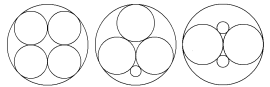
\includegraphics[width=0.5 \textwidth]{9.png}
					\caption{放置方法}
				\end{figure}
				
			\subsubsection{算法讨论}
				如果 $d$ 是合法的解,那么更大的解 $d + \Delta, \Delta > 0$ ,其仍然合法。故可先二分答案,检查某个特定的 $d$ 是否合法。	
				
				不妨枚举放入的顺序,设 $d_1, d_2, d_3, d_4 $ 先后放入其中。
				
				如果 $d < d_1$ 那么显然这个解是不合法的。否则可以贪心的将其放在容器的边缘。随后依次将后面的圆,与前面的某两个圆相切地,不重合地放入内。具体与哪两个圆相切,需要枚举。如果能够放下四个圆,那么返回有解。如果不行,更改放入的顺序继续搜索。如果无论如何都不行,那么只能返回无解。
				
				贪心的正确性可用调整法粗略地证明。如果某一个圆只与一个圆相切,或者完全不相切,那么在不与其他圆重合的情况下,稍稍移动一点,就可以与至少两个圆重合。
				
				配合二分搜索,即可求知答案。
			\subsubsection{时空复杂度}
				
				时间复杂度 $\mathcal{O}\left(k\right)$。$k$ 是二分次数,与精度相关。由于只有四个圆,搜索出来的情况数非常有限,并且是常数,故没有写入时间复杂度上限。
					
				空间复杂度 $\mathcal{O}\left(1\right)$。
		\newpage
		\subsection{ACM/ICPC World Finals 2009 G House of Cards}
			\subsubsection{题目大意}
				一个扑克游戏。洗好一碟 $2 M$ 张牌。牌有点数(1 到 13)和花色(赤黑)之分。先用八张牌按顺序摆成图 \ref{2009G} 所示的样子,作为起始局面。随后两个人(赤黑)顺次抽牌。第一张牌的颜色决定先手。每个人可以
				\begin{enumerate}
					\item 保留当前拿着的牌,并视之为保留牌(要在手中没有保留的牌时);
					\item 在两张构成谷的牌上横着搭一张,变为平的;如果手中还有有一张牌,则视之为保留牌;或者
					\item  在平的地方用保留牌和抽到的牌搭一个峰。
				\end{enumerate}
				每次执行后两个操作形成三角后,对应的三张牌的点数之和将会作为分数,加入到这三张牌中,最多的颜色对应的人上。分多的人获胜。
				
				两人均使用最优策略,试问赤黑两人谁能获胜。
				
				$M \le 13$。
				\begin{figure}[htb]
					\centering
					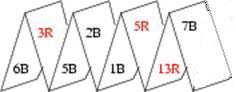
\includegraphics[width=0.3 \textwidth]{10.png}
					\caption{可能的开始局面}\label{2009G}
				\end{figure}
				
			\subsubsection{算法讨论}
				大方向是 博弈搜索 与 $\mathrm{\alpha}$-$\mathrm{\beta}$ 剪枝。将结果视为黑的得分减去赤的得分,那么黑就会最大化该值,赤最小化该值,套用博弈搜索即可知道结果。
				
				讨论下博弈搜索的细节。最多有 $2M$ 个牌位,其中 $8$ 个已固定,那么剩余的牌会产生远远不足 $(2M - 8 + 1)^2 \cdot(2M - 8)! \le 19^2 18!$ 的状态,配合$\mathrm{\alpha}$-$\mathrm{\beta}$ 剪枝,状态数会更少。应该可以通过测试。
			
			\subsubsection{时空复杂度}
				忽略 $\mathrm{\alpha}$-$\mathrm{\beta}$ 剪枝,时间复杂度 $\mathcal{O}\left(M^2 \cdot (2M)!\right)$。 $\mathrm{\alpha}$-$\mathrm{\beta}$ 剪枝非常有效,实际情况远远不足该上限。
					
				空间复杂度 $\mathcal{O}\left(1\right)$。
		\newpage
		\subsection{ACM/ICPC World Finals 2009 H The Ministers’ Major Mess}
			\subsubsection{题目大意}
				有 $N$ 项决议,$M$ 个人对其中 $k, k \le 4$ 项决议投票(同意或反对)。请确定哪些决议需要实施,哪些协议不许实施,使得每个人的投票中,有\emph{超过}半数的项目都得以满足。需要确定哪些决议必须通过,那些决议不许通过,哪些决议可通过可不通过;或者直接返回无解。			
				
				$N \le 100, M \le 500$。
			\subsubsection{算法讨论}	
				类似于  \textit{POI 2001 Peaceful Commission },转为 $2\text{-SAT}$。
				
				具体地,对于 $k = 1, 2$ 的人,其投票的内容是板上钉钉的事,故对于每一票 $x$,添加条件 $\bar{x} \rightarrow x$。$\rightarrow$ 表示蕴含,$A \rightarrow B = \neg A \vee B$。$\bar{x}$ 是 ${x}$ 的对立事件。
				
				对于 $k = 3, 4$ 的人,至多有一票被违背,故设其投票 $x_1, x_2, \ldots, x_k$,则添加条件
$\bigwedge_{i \ne j} (\bar{x_i} \rightarrow x_j) = 1$。
				
				此 SAT 问题的解与原问题的解一一对应。根据  $2\text{-SAT}$  的解法和相关推论,建好图后,若某 $\bar{x}, x$ 位于同一强连通块,则问题无解。否则肯定是有解的。
				
				若对于某一决议 $x$,$x \rightarrow \bar{x}$,即对应结点存在有向路径,那么显然 $x$ 不能被通过;反之 若 $x \leftarrow \bar{x}$,则其必须被通过。
				
				而如果 $x, \bar{x}$ 间无任何逻辑关系(对应点根本不连通),则 $x$ 可通过可不通过,因为考虑到求解 SAT 问题时,会先拓扑排序,然后根据拓扑序先入为主地确定哪些结点被选择。既然目前对应点根本不连通,则其都有可能在拓扑序中靠前地被选择,故都有可能构造出一个可能的合法解。
				
				根据以上的分析,求两点间的连通性,可判定出答案。
			\subsubsection{时空复杂度}
				时间复杂度 $\mathcal{O}\left(N(N + M)\right)$。
					
				空间复杂度 $\mathcal{O}\left(N + M\right)$。
		\newpage
		\subsection{ACM/ICPC World Finals 2009 I Struts and Springs}
			\subsubsection{题目大意}
				问题描述了一个在嵌套的窗口中,主窗口尺寸了发生改变后,子窗口的尺寸的变化的棍棒弹簧响应机制。
				
				对于每个子窗口,其向父窗口在对应的四个边缘上连接了四条线,同时此窗口的底部和顶部,左侧和右侧也分别连了线。每条线均可能是棍棒或弹簧。外层窗口移动时,内层窗口的变化服从物理原理,即棍棒的长度不会变化,而弹簧的变化服从胡克定律,即同一方向的弹簧等比例伸缩。如果某一方向上三条线都是棍棒,则最上或最右的棍棒变为弹簧。
				
				给定窗口的初始位置,请模拟这个响应机制的结果。
				
				窗口数 $N \le 100$,尺寸变化操作次数 $\le 100$。.
				
			\subsubsection{算法讨论}	
				先需要根据窗口位置,确定窗口父子关系。简单的 $\mathcal{O}\left(N^2\right)$ 的暴力就可以解决。先枚举一个窗口,则包围了他的,且面积最小的就是其父窗口。
				
				随后根据题目中表述的模型直接模拟即可。注意到除了主窗口外,其他的窗口左上角的坐标还会有偏移,在递归时须考虑到。
			
			
			\subsubsection{时空复杂度}
				时间复杂度 $\mathcal{O}\left(N^2 + NM\right)$。
					
				空间复杂度 $\mathcal{O}\left(N\right)$。
		\newpage
		\subsection{ACM/ICPC World Finals 2009 J Subway Timing}
			\subsubsection{题目大意}
				给定树 $T = (V, E)$。给定边权 $W^* : E \mapsto \mathbb{N}$。试求另外求一个边权 $W : E \mapsto \mathbb{N}$ 使得
				\begin{align}
					\forall x \in E,\quad & | W(x) - W^*(x) / 60 | < 1  \label{2009J1}
				\end{align}
				且
				\begin{align}
					Ans = \max_{u, v \in V} 60 \; |W(u, v) - W^*(u, v) / 60 |
				\end{align}
				最小化。其中 $W(u, v), W^*(u, v)$ 分别表示 $W, W^*$ 意义下两点间的距离。 
				
				点数 $N = |V| \le 100$
			\subsubsection{算法讨论}	
				\begin{theorem}
					$Ans < 120$。
				\end{theorem}
				\begin{pf}
					我们将给出一个使得 $\forall u, v \in V,\,  60\; |W(u, v) - W^*(u, v) / 60 | < 120$ 的 $W$ 来完成证明。
					
					任意选一个点标记为 $1$,并作为根。再设 $d(x) =\left\lfloor W^*(1, x) / 60 + 0.5 \right\rfloor$,这样 $e = (u, v), u $ 是父亲 $, W(e) = d(v) - d(u)$ 就符合条件。
					
					先说明其满足要求  \eqref{2009J1}。因为  $d(x) =\left\lfloor W^*(1, x) / 60 + 0.5 \right\rfloor$,则
					\begin{align}
						- 0.5 & \le W^*(1, u)  / 60 - d(u) <0.5 \label{2009JA} \\
						- 0.5 & \le W^*(1, v)  / 60 - d(v) < 0.5 \label{2009JB}
					\end{align}
					$\eqref{2009JA}  + (- \eqref{2009JB})$
					\begin{align}
						-1  < W(u, v) - W^*(u, v) / 60 < 1 \label{2009JC} 
					\end{align}
				
					我们再说明  $\forall u, v \in V, \, 60\; |W(u, v) - W^*(u, v) / 60 | < 120$。设 $u, v$ 的最近公共祖先为 $l$,使用与得出 \eqref{2009JC} 类似的方法,同理可推知
					\begin{align}
						60\; |W(u, v) - W^*(u, v) / 60| & = 60\; |W(l, u) - W^*(l, u) / 60 + W(l, v)  - W^*(l, v) / 60|
						\notag \\
							& \le
							60 \;\left( |W(l, u) - W^*(l, u) / 60| + |W(l, v)  - W^*(l, v) / 60| \right)\notag \\
							& < 60 \;(1 + 1)=  120
					\end{align} \qed
					
				\end{pf}
				又由于问题具有单调性,故我们可以以 $120$ 为上限,枚举答案 $Ans^\prime$,并检验。
				
				定义状态 $F[i][j]$ 表示在 $i$ 为根的子树中,满足
				\begin{enumerate}
					\item $\forall$ 路径  $ u, v, \quad 60 \;|W(u, v) - W^*(u, v) / 60 | \le ^\prime$;且
			 		\item $\forall $ 子树中的 $ v \in V, $ 路径 $i, v, \quad -j \le 60 \;( W(i, v) - W^*(i, v) / 60 ) \le F[i][j]$;
				\end{enumerate}
				的最小$ F[i][j]$。这个问题有点类似背包问题,每条父子边有两个状态——$W^*(i, v) / 60$ 向上或向下取整。根据枚举出的取整情况,可以推知状态转移方程。具体的,设 $60 \;( W(i, v) - W^*(i, v) / 60 ) = \Delta $,则 % 有转移过程:
				\begin{algorithm}[H]
				\caption{已知 $i$ 儿子的 $F[\cdot][\cdot]$,求 $F[i][\cdot]$ }
				\label{}
					\begin{algorithmic}[1]
						\State $F[i][\cdot] \gets 0$
						\For{儿子 $v$}
							\State $G[\cdot] \gets + \infty$
							\For{$\Delta$}
								\For{$0 \le k \le Ans^\prime$}
									\For{$0 \le j \le Ans^\prime \land k + j - \Delta \le Ans^\prime$ }
										\If{ $F[i][k] + F[v][j] + \Delta  \le Ans^\prime $}
											\State $G[\max(k, j - \Delta)] \gets \min(G[\max(k, j - \Delta)], \max(F[i][k], F[v][j] + \Delta))$
										\EndIf
									\EndFor
								\EndFor
								\State $F[i] \gets G$
							\EndFor
						\EndFor
					\end{algorithmic}
				\end{algorithm}
				须具体处理边界的溢出问题。
				
				如果存在 $i \le Ans^\prime$ 使得 $F[1][i] \le Ans^\prime$ 则问题有解;反之,问题无解。套回去用二分答案求解
%				即可
				。

%				\begin{align}
%					\text{枚举儿子} \, v \atop \Delta   F[i][j] \gets \min(F[)
%				\end{align}

			\subsubsection{时空复杂度}
				时间复杂度 $\mathcal{O}\left(N\right)$。此处隐含常数 $\log_2 120 \times 2 \times 120 \times 120$。
					
				空间复杂度 $\mathcal{O}\left(N\right)$。此处隐含常数 $120$。
		\newpage
		\subsection{ACM/ICPC World Finals 2009 K Suffix-Replacement Grammars}
			\subsubsection{题目大意}
				后缀替换文法是指给定一些替换文法
				\begin{align}
					A \rightarrow B, \; |A| = |B|
				\end{align}
				只要字符串 $S$ 的后缀有 $A$ 则可将其替换为 $B$。		
				给定两个单词 $S, T$,问		$S \rightarrow T$ 需要至少几次后缀替换。 字符串只含拉丁字母。
				
				$|S| = |T| \le 20, $ 文法数 $ K \le 100$。
			\subsubsection{算法讨论}	
				容易看出题目对应一个图论问题。将单词视为结点,文法视为边,则答案等价于询问某两点间的最短路。稍加构造便知,答案有可能上亿,BFS 算法是行不通的。故目前解决问题的当务之急是利用后缀这一特性,将图做某种变换,加速 BFS。
				
				我们定义一个小一点的图 $G_L = (V_L, E_L), L \le |S|$,其中$V_L$ 是长度为 $L$ 的字符串集,$E_L$ 是长度\emph{不超过} $L$ 的后缀替换文法集。也就是说,一开始我们提到的图就表示为 $G_{|S|}$。
				
				由于我们只关心  $G_L $ 中两个点的距离,故我们可以稍稍简化一下  $G_L$。方法如下
				\begin{enumerate}
					\item 从 $E_L$ 中删除所有长度\emph{低于} $L$ 的后缀替换文法;
					\item 对于某两个首字母相同的字符串 $s, t$ ,连一条有权值的边,权值为 $G_{L - 1}$ 中,删掉 $s, t$ 首字母后对应的点间的距离;
					\item 对于原来未设权值的边将权值设置为 1。
				\end{enumerate}
				显然修改后不会改变答案,且类似于动态规划,合并了一些中间状态,减少了实际经过的边的数量。此外忽略耗费的时间,从 $G_1, G_2, ...$ 依次算到 $G_|S|$ 是可以求出答案的。接下来,我们还需要减少点的数量,来完成任务。
				
				由于我们只关心 $G_{|S|}$ 中 $S, T$ 两点的距离。而 $S $ 到 $ T$ 不管怎么变,都不会脱离这 $K$ 个文法。
				也就是说真正有用的点(字符串),是这  $K$ 个文法中 $2 K$ 个字符串,加上 $S, T$ 总计 $(2 K + 2)$ 个字符串的后缀。换言之我们只需要建 $|S|$ 张图,每张图 $(2 K + 2)$  个结点就足以完成运算。带权最短路可以用 Floyd-Warshall 算法。
				
				需要注意答案可能超出 32 位整型。
			\subsubsection{时空复杂度}
				时间复杂度 $\mathcal{O}\left(|S| K^3 \right)$。
					
				空间复杂度 $\mathcal{O}\left(K^2 \right)$。
		\newpage

	
	\section{ACM/ICPC World Finals 2008}
		\subsection{ACM/ICPC World Finals 2008 A Air Conditioning Machinery}
			\subsubsection{题目大意}
				如图 \ref{2008aaa},有一个 $N \times M \times K$  的空调。上有一个进风口一个出风口。试用不超过六个管道零件,拼接一个管道,至于空调\emph{内部},并连接两个风口,并输出最少需使用的管道数量。
					
				\begin{figure}[htb]
					\centering
					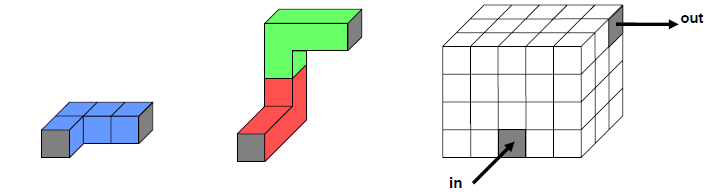
\includegraphics[width=0.7 \textwidth]{2008a.png}
					\caption{管道零件,管道,空调} \label{2008aaa}
				\end{figure}
			
			\subsubsection{算法讨论}
				暴力搜索,根据目前管子已经接到的位置,枚举下一个零件的方向(4 个),接长的一端还是短的一端(2 个)。注意管子不能超出空调外部,或与前面的管子重合。
					
				总搜索量不超过 $(4 \times 2) ^ 6$。
			
			
			\subsubsection{时空复杂度}
				
				时间复杂度 $\mathcal{O}\left(1\right)$。内含常数  $(4 \times 2) ^ 6 = \num{262144} $。
					
				空间复杂度 $\mathcal{O}\left(NMK\right)$。
		\newpage
		\subsection{ACM/ICPC World Finals 2008 B Always an Integer}
			\subsubsection{题目大意}
				给定若干形如
				\begin{align}
					P(x) = \frac{1}{b} \left( a_nx^n + a_{n - 1} x^{n - 1} + a_{n - 2} x^{n - 2}  + \cdots + a_{0} % x^{0} 
					  \right)
				\end{align}
				的 $n$ 次多项式,$a_i, b$ 均为整数。试问对于所有整数 $x \in \mathbb{Z}$ 是否都有 $P(x) \in \mathbb{Z}$。
				
				$n \le 100$。
			\subsubsection{算法讨论}
				\begin{theorem}
					$\forall x \in \mathbb{Z}, P(x) \in \mathbb{Z}$ 的充要条件是
					$\forall x \in \mathbb{Z} \cap [0, n], P(x) \in \mathbb{Z}$。
				\end{theorem}
				\begin{pf}
					后者的条件严于前者,故必要性显然,下证充分性。
					
%					将函数视为序列。
					定义差分 $\Delta [P](x) = P(x + 1) - P(x)$。再定义高阶差分 $\Delta^k [P](x) = \Delta^{k - 1} [P](x + 1) - \Delta^{k - 1} [P](x) $,特别地 $\Delta^0 [P](x) = P(x)$。
						
					容易验证,$\Delta^k [P](x), 0 \le k \le n$ 是一个 $(n - k)$ 次多项式,换言之,$\Delta^n [P](x)$ 是常函数。
					
					而如果确定了 $P(0), P(1), \ldots, P(n)$ 的值,就可以根据定义计算出 $\Delta^n [P](0)$ 指向的这个常数,从而推知整个 $\Delta^n [P](x)$,并倒推出所有 $\forall x \in \mathbb{Z}$ 的 $\Delta^{n - 1} [P](x) , \Delta^{n - 2} [P](x), \ldots$ ,直到原函数 $ \Delta^{0} [P](x)$。
					而整个过程我们只使用了对整数封闭的差分运算(加减运算),故只要一开始的 $P(0), P(1), \ldots, P(n)$  都是整数,那么 最终计算出的 $ \Delta^{0} [P](x)$ 所有整点就都是整数。% 故差分运算  $\Delta$ 对满足条件 
					\qed
				\end{pf}
				故我们只需对 $x \in \mathbb{Z} \cap [0, n]$ 进行检验。检验的方法是判断
				\begin{align}
					 \left( a_nx^n + a_{n - 1} x^{n - 1} + a_{n - 2} x^{n - 2}  + \cdots + a_{0} % x^{0} 
					  \right) \equiv 0 \pmod{b}
				\end{align}
				是否都成立,若是,答案则为是;反之答案为否。
			\subsubsection{时空复杂度}
				
				时间复杂度 $\mathcal{O}\left(n^2\right)$。
					
				空间复杂度 $\mathcal{O}\left(n\right)$。
		\newpage
		\subsection{ACM/ICPC World Finals 2008 C Conveyor Belt}
			\subsubsection{题目大意}
					如图 \ref{2008c},有若干齿轮,每个齿轮有规定的旋转方向。指定起点到终点,试用履带从起点连接到终点,使得
					\begin{enumerate}
						\item 符合齿轮旋转方向;
						\item 履带之间,以及履带和齿轮不交叉、重叠;
						\item 履带未与齿轮接触的部分,要求每一段的长度\emph{小于} $d$;且
						\item 履带总长最短。
					\end{enumerate}
					求这个总长度。
					
					齿轮数 $N \le 20$。
				\begin{figure}[htb]
					\centering
					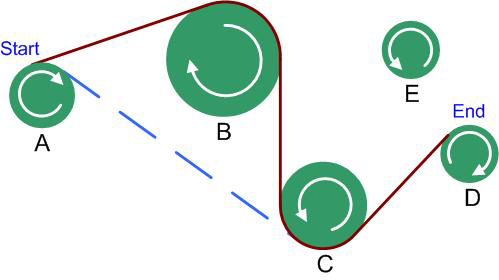
\includegraphics[width=0.6 \textwidth]{2008c.png}
					\caption{轮轴和履带} \label{2008c}
				\end{figure}
				
			\subsubsection{算法讨论}
				不妨先解决几何方面的问题。
				
				一个是两个轮轴间的连线,显然应为其公切线。具体是内公切线,还是外公切线,需根据两个轮轴的方向来确定。为讨论方便,可设顺时针的半径为负。这样设对应公切线的切点相对于圆心角度为 $\theta$,则应当满足方程
				
				\begin{align}
					((x_1 +r_1 \cos \theta)- (x_2 +r_2 \cos \theta), (y_1 +r_1 \sin \theta)-(y_2 +r_2 \sin \theta)) \cdot ( \cos \theta,  \sin \theta) = 0 \label{2008a}
				\end{align}
				因为切线应与圆心到切点的直线垂直。其中 $\cdot$ 是内积运算,$(a, b) \cdot (c, d) = ac + bd$。解  \eqref{2008a} 的方法是先化简为 
				\begin{align}
					(x_1 - x_2) \cos \theta + (y_1 - y_2) \sin \theta & = - (r_1 - r_2)
					\intertext{令 $d = \sqrt{(x_1 - x_2)^2 + (y_1 - y_2)^2}, (\cos \phi, \sin \phi) = ((x_1 - x_2) /d, (y_1 - y_2) / d)$,得}
					d \cos \left(\phi - \theta \right) & =  - (r_1 - r_2)
				\end{align}
				$\phi$ 和 $\theta$ 均可以用反三角求出。注意 $\theta$ 有两个解,具体取哪个根据方向确定。
				
				然后是线线和线圆的交叉的判定。前者用叉积即可判断。后者可以先将直线写成参数方程 $\mathbf{p} = \mathbf{a} + \mathbf{v} t$,代入圆方程 $ \left(\mathbf{p} - \mathbf{q}\right)^2 = r^2$,求解二次方程。根据解来判断。
					
				预处理好几何信息后,爆搜即可。注意需用交叉等减枝。
				
			\subsubsection{时空复杂度}
				时间复杂度 $\mathcal{O}\left(N^3\right)$ 几何预处理(此处没有履带交叉的检测) $+ $$ \mathcal{O}\left(N! N^2\right)$ 爆搜。题目限制繁多,致使实际有效状态并没有这么多。
					
				空间复杂度 $\mathcal{O}\left(N^2\right)$(某两个轮轴能否连边)。

		\newpage
		\subsection{ACM/ICPC World Finals 2008 E Huffman Codes}
			\subsubsection{题目大意}
				已知若干个字母的 Huffman 码,求有多少中频率分布能生成这样的  Huffman 码。约定频率为整百分数。频率小的都在左子树。
				
				字符数 $|\Sigma| = N \le 20$。
				
			\subsubsection{算法讨论}
				大致方向是爆搜。根据  Huffman 码,可以建立出  Huffman 树。
				
				约定右子树(1)优先访问,那么  Huffman 树的 BFS 序列的评论是单调下降的;反之亦然。具体的证明分两步。
				%可用调整法。
				第一步是要证明不同层的频率间大小关系的充要性,这个根据  Huffman 码构造时不断选择较小的频率合并不难证明,或者调整法,交换某两层的点后,会致使 Huffman 码不优(平均长度 $\sum{p_il_i}$ 没达到最小值);第二步是要说明同一层左边到右边的点的频率大小关系的充要性,这个是由于题目规定了频率小的都在左子树。此结论可以很大程度的加快搜索速度。
				
				随后爆搜就可以了。同一个父亲的两个节点的频率加起来要和父亲的相等,且须满足前面的结论。
				
			\subsubsection{时空复杂度}
				时间复杂度涉及到一个很困难的组合计数,并且还需考虑减枝,不易于表达成大 $\mathcal{O}$ 记法。不过考虑到 $N \le 20$,爆搜的速度应该还是很快的。
				
				空间复杂度 $\mathcal{O}\left(N\right)$。
			
		\newpage
		\subsection{ACM/ICPC World Finals 2008 F Glenbow Museum}
			\subsubsection{题目大意}	
				\begin{wrapfigure}{r}{0.25 \textwidth}
					\centering\vskip-2em
					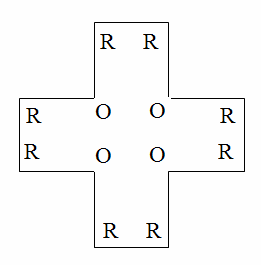
\includegraphics[width=0.23 \textwidth]{2008f.png}
					\caption{拐角表示法} \label{2008f}
				\end{wrapfigure}
					
				每个正交简单多边形,都可用如图所示的拐角表示法表示。(R)ight = 直角,(O)btuse = 钝角。逆时针将 RO 串起来得到的串就是 RO 串。
				
				定义一个 RO 串是需要计数的,当且仅当存在一个图形,其拐角表示法对应这个 RO 串,且内有一点可以“看”到所有边界。
				
				问所有的长度为 $N$ 的 RO 串中,有多少个是需要计数的。
				
			\subsubsection{算法讨论}

				\begin{theorem}
					问题等价于问所有的长度为 $N$ 的 RO 串中,有多少个的 R 比 O 多 4 个,且无连续两个 O。
				\end{theorem}
				\begin{pf}
					先说明 R 必须比 O 多 4 个。由于必须是简单多边形,故其旋转数为 $1$。分析可知,一个 R 的旋转数为 $\frac{1}{4}$ 而一个 O 的旋转数为 $-\frac{1}{4}$,故 R 必须比 O 多 4 个。
										\begin{figure}[htb]
					\centering
\definecolor{ffzzzz}{rgb}{1,0.6,0.6}
\definecolor{zzwwff}{rgb}{0.6,0.4,1}
\definecolor{zzttqq}{rgb}{0.6,0.2,0}
\definecolor{xdxdff}{rgb}{0.49,0.49,1}
\definecolor{qqqqff}{rgb}{0,0,1}
\definecolor{cqcqcq}{rgb}{0.75,0.75,0.75}



\centering
\begin{minipage}{.3\textwidth}
  \centering

\begin{tikzpicture}[line cap=round,line join=round,>=triangle 45,x=1.0cm,y=1.0cm,scale = 0.3]
\draw (4,20)-- (4,24);
\draw (4,24)-- (6,24);
\draw (6,24)-- (6,20);
\draw [->,color=ffzzzz] (4,22) -- (2,22);
\draw [->,color=ffzzzz] (6,22) -- (8,22);
\begin{scriptsize}
\if false
\fill [color=zzwwff] (4,20) circle (2.5pt);
\fill [color=zzwwff] (4,24) circle (2.5pt);
\fill [color=zzwwff] (6,24) circle (2.5pt);
\fill [color=zzwwff] (6,20) circle (2.5pt);
\fill [color=zzwwff] (2,22) circle (2.5pt);
\fill [color=zzwwff] (4,22) circle (2.5pt);
\fill [color=zzwwff] (6,22) circle (2.5pt);
\fill [color=zzwwff] (8,22) circle (2.5pt);
\fi

\end{scriptsize}

\end{tikzpicture}

  \captionof{figure}{}
  \label{fig:2008c1}
\end{minipage}%
\begin{minipage}{.7\textwidth}
  \centering
\definecolor{ffzzzz}{rgb}{1,0.6,0.6}
\definecolor{ttqqqq}{rgb}{0.2,0,0}
\definecolor{zzttqq}{rgb}{0.6,0.2,0}
\begin{tikzpicture}[line cap=round,line join=round,>=triangle 45,x=1.0cm,y=1.0cm, scale = 0.3]
\fill[color=zzttqq,fill=zzttqq,fill opacity=0.1] (1,6) -- (1,2) -- (2,2) -- (2,1) -- (5,1) -- (5,0) -- (9,0) -- (9,3) -- (10,3) -- (10,4) -- (11,4) -- (11,5) -- (10,5) -- (10,7) -- (3,7) -- (3,6) -- cycle;
\fill[color=zzttqq,fill=zzttqq,fill opacity=0.1] (14,6.8) -- (14,0.4) -- (14.2,0.4) -- (14.2,0.2) -- (14.4,0.2) -- (14.4,0) -- (23.6,0) -- (23.6,3) -- (23.8,3) -- (23.8,4) -- (24,4) -- (24,6.8) -- (23.8,6.8) -- (23.8,7) -- (14.2,7) -- (14.2,6.8) -- cycle;
\draw [color=zzttqq] (1,6)-- (1,2);
\draw [color=zzttqq] (1,2)-- (2,2);
\draw [color=zzttqq] (2,2)-- (2,1);
\draw [color=zzttqq] (2,1)-- (5,1);
\draw [color=zzttqq] (5,1)-- (5,0);
\draw [color=zzttqq] (5,0)-- (9,0);
\draw [color=zzttqq] (9,0)-- (9,3);
\draw [color=zzttqq] (9,3)-- (10,3);
\draw [color=zzttqq] (10,3)-- (10,4);
\draw [color=zzttqq] (10,4)-- (11,4);
\draw [color=zzttqq] (11,4)-- (11,5);
\draw [color=zzttqq] (11,5)-- (10,5);
\draw [color=zzttqq] (10,5)-- (10,7);
\draw [color=zzttqq] (10,7)-- (3,7);
\draw [color=zzttqq] (3,7)-- (3,6);
\draw [color=zzttqq] (3,6)-- (1,6);
\draw [color=zzttqq] (14,6.8)-- (14,0.4);
\draw [color=zzttqq] (14,0.4)-- (14.2,0.4);
\draw [color=zzttqq] (14.2,0.4)-- (14.2,0.2);
\draw [color=zzttqq] (14.2,0.2)-- (14.4,0.2);
\draw [color=zzttqq] (14.4,0.2)-- (14.4,0);
\draw [color=zzttqq] (14.4,0)-- (23.6,0);
\draw [color=zzttqq] (23.6,0)-- (23.6,3);
\draw [color=zzttqq] (23.6,3)-- (23.8,3);
\draw [color=zzttqq] (23.8,3)-- (23.8,4);
\draw [color=zzttqq] (23.8,4)-- (24,4);
\draw [color=zzttqq] (24,4)-- (24,6.8);
\draw [color=zzttqq] (24,6.8)-- (23.8,6.8);
\draw [color=zzttqq] (23.8,6.8)-- (23.8,7);
\draw [color=zzttqq] (23.8,7)-- (14.2,7);
\draw [color=zzttqq] (14.2,7)-- (14.2,6.8);
\draw [color=zzttqq] (14.2,6.8)-- (14,6.8);
\end{tikzpicture}
  \captionof{figure}{转化 的例子}
  \label{fig:2008c2}
\end{minipage}
\end{figure}

					再说明 不能有相邻的 O。原因也很简单,如果有,那么就能形成如图 \ref{fig:2008c1} 所示的图形,半平面交肯定为 $\varnothing$。
					
					最后说明只要 R 比 O 多 4 个,且无连续两个 O,就能找到这样的一个简单多边形。我们可以先随意画出一个拐角表示法为该序列的简单多边形。然后固定最靠上、下、左、右的边,通过将另外的边缩短为无穷小的方法,将其变化成一个趋近于长方形的图形。由于没有两个连续的 O ,故边界上也就没有无限小的内凹。此时只要这个图形无线趋近于长方形,那么其中点(重心)就无限趋近于满足要求。这个无限趋近于长方形的图形就是我们要找的。
				\end{pf}
				这样就变成了一个计数问题。如果 $N$ 为奇数,则答案为 $0$;否则答案
				\begin{align}
					Ans = \binom{N/2 + 1}{3} + 2 \binom{N/2 + 1}{4} \label{2008feq}
				\end{align}
				\eqref{2008feq} 的得出方法是通过枚举首尾的字母情况,再使用隔板法。
					
			\subsubsection{时空复杂度}
				时空复杂度 $\mathcal{O}\left(1\right)$。


		\newpage
\subsection{ACM/ICPC World Finals 2008 G Net Loss}
		\subsubsection{题意概述}
			给定多项式 $p(x)$ 和常数 $c \left(-1 < c < 1\right)$,求三个实数 $k_1,k_2,b$ 使得
			\begin{align}
				d = \int_{-1}^{c} \left(k_1\left(x-c\right)+b - p(x)\right)^2 \mathrm{d}x
					+ \int_{c}^{1} \left(k_2\left(x-c\right)+b - p(x)\right)^2 \mathrm{d}x 
			\end{align}
			最小化,并输出 $k_1,k_2,b$ 的值。
			
			$1 \le p(x) \text{的次数} \le 10$。多组询问。
			
		\subsubsection{简要分析}
			考虑 $d$ 关于 $k_1,k_2,b$ 的梯度
			\begin{align}
				\nabla d & = \left(\frac{\mathrm{\partial} d}{\mathrm{\partial} k_1},
						\frac{\mathrm{\partial} d}{\mathrm{\partial} k_2},
						\frac{\mathrm{\partial} d}{\mathrm{\partial} b}\right) 
			\end{align}
			其中
			\begin{align}
					\frac{\mathrm{\partial} d}{\mathrm{\partial} k_1} 
						& = \int_{-1}^{c} 2(k_1(x-c)+b-p(x)) \cdot (x-c) \; \mathrm{d}x\\
					\frac{\mathrm{\partial} d}{\mathrm{\partial} k_2} 
						& = \int_{c}^{1} 2(k_2(x-c)+b-p(x)) \cdot (x-c) \; \mathrm{d}x\\
					\frac{\mathrm{\partial} d}{\mathrm{\partial} b} 
						& = \int_{-1}^{c} 2(k_1(x-c)+b-p(x)) \; \mathrm{d}x +
							\int_{c}^{1} 2(k_2(x-c)+b-p(x)) \; \mathrm{d}x 
			\end{align}
			由三个方向的偏导随该维的单调性可知,$d$ 取得最小值当且仅当
			\begin{align}
				\nabla d = \mathbf{0}
			\end{align}
			即
			\begin{align}
				\left\{\setlength{\tabcolsep}{2.5pt}
					\begin{tabular}{cccccccc}
						$\displaystyle k_1 \int_{-1}^{c} (x-c)^2 \; \mathrm{d}x$ & $+$ & $0$ & $+$ & $\displaystyle b \int_{-1}^{c} (x-c) \; \mathrm{d}x $  &$ =$&$\displaystyle  \int_{-1}^{c} p(x)\cdot(x-c) \; \mathrm{d}x$ \\
						$0$ & $+$ & $\displaystyle k_2 \int_{c}^{1} (x-c)^2 \; \mathrm{d}x$ &$ +$&$ \displaystyle b \int_{c}^{1} (x-c) \; \mathrm{d}x $&$  =$ &$ \displaystyle \int_{c}^{1} p(x)\cdot(x-c) \; \mathrm{d}x$ \\
						$k_1 \displaystyle \int_{-1}^{c} (x-c) \; \mathrm{d}x$ & $+$ & $k_2\displaystyle \int_{c}^{1} (x-c) \; \mathrm{d}x$ &$ +$&$ b \displaystyle \int_{-1}^{1} \mathrm{d}x $&$  =$ &$ \displaystyle \int_{-1}^{1} p(x) \; \mathrm{d}x$ 
					\end{tabular}
				\right.
			\end{align}
			写成矩阵的形式
			\begin{align}
				A\mathbf{x} = \mathbf{b}
			\end{align}
			其中
			\begin{align}
				A & = \begin{bmatrix}
					\displaystyle \int_{-1}^{c} (x-c)^2 \; \mathrm{d}x & 0 & \displaystyle\int_{-1}^{c} (x-c) \; \mathrm{d}x \\
					0 & \displaystyle\int_{c}^{1} (x-c)^2 \; \mathrm{d}x &\displaystyle \int_{c}^{1} (x-c) \; \mathrm{d}x \\
					\displaystyle\int_{-1}^{c} (x-c) \; \mathrm{d}x & \displaystyle\int_{c}^{1} (x-c) \; \mathrm{d}x & 2
				\end{bmatrix} \\
				\mathbf{x} & = (k_1,k_2,b)^{\mathrm{T}} \\
				\mathbf{b} & = \left(\int_{-1}^{c} p(x)\cdot(x-c) \; \mathrm{d}x,
					\int_{c}^{1} p(x)\cdot(x-c) \; \mathrm{d}x,
					\int_{-1}^{1} p(x) \; \mathrm{d}x\right)^{\mathrm{T}}
			\end{align}
			定积分可以使用牛顿—莱布尼兹定理求得。剩下的只需使用高斯消元,人工解方程,或者通过伴随矩阵求逆矩阵等方法求出解向量 $\mathbf{x}$。
			
			计算可得,系数矩阵 $A$ 的行列式 $\left|A\right| = \textstyle \frac{1}{18} (1+c)^3 (1-c)^3 $,故 $\left|A\right|  > 0 $ 恒成立,方程组恒有且仅有一组解。
				
			\subsubsection{时空复杂度}
				时间复杂度 $\mathcal{O}\left(p(x) \text{的次数}\right)$。
				
				空间复杂度 $\mathcal{O}\left(p(x) \text{的次数}\right)$。
		
		\newpage
		\subsection{ACM/ICPC World Finals 2008 H Painter}
		\subsubsection{题意概述}
			如图  \ref{2008h} 有一堆三角形。判断三角形的边界是否有重叠(端点重合也算)。如果没有,再判断三角形迭代了最多几层。

				三角形数 $n \le 100000$。
				
				
				\begin{figure}[htb]
					\centering
					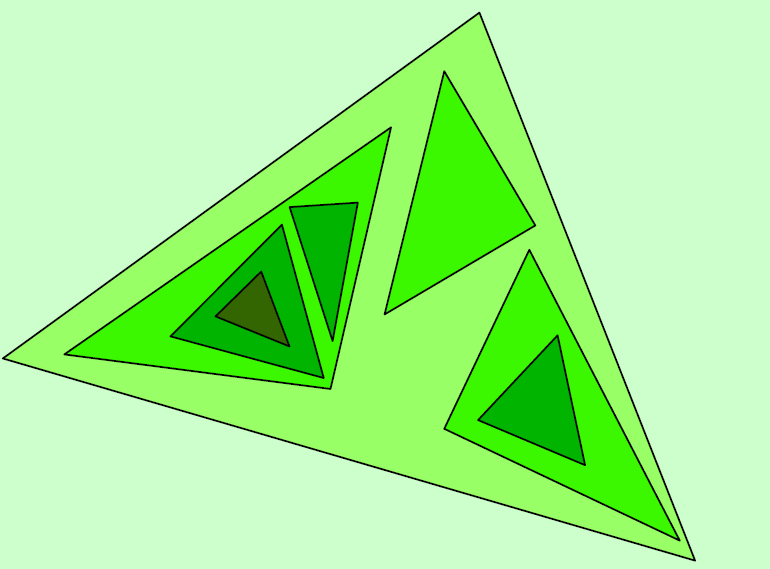
\includegraphics[width=0.4 \textwidth]{2008h.png}
					\caption{可能的三角形集} \label{2008h}
					\vskip-1em
				\end{figure}
				
		\subsubsection{简要分析}
				整个问题都可以用扫描线解决。
				
				设没有竖直的边(若有,则旋转某一角度),那么从左到右扫描,三角形就是一个从点,线性地变化为一个区间,再变成一个一个点,最后消失的动态区间。而同理直线就是动点。
				
				不妨用平衡树来维护整个扫描线,那么一个新三角形出现在扫面线上时,需要加两个动点。为了避免交叉,需要与其前一个和后一个动点所在的直线进行交叉检测。而对于其他点,我们可以保证目前(在前一个点或后一个点删除之前)不会交叉,因为如果交叉,其必然会与相邻点交叉,而不会跨过这两个点。
				
				同样地,删除时,需对待删除点的相邻两条直线先进行交叉检测,再删除。
				
				交叉检测使用叉积来判定,且 需小心处理端点。如果有任何一次的交叉检测不通过,那么就立即返回边界重叠,退出程序。
				
				如果没有重叠的边界,那么我们可以继续借助前面辅助线的信息,在插入三角形(两个动点)前维护其父子关系;或者我们只关心其深度,故维护好次深度即可。不妨将三角形的上边界看为 $+ 1$,下边界看为 $- 1$。那么要求得深度,只需对在当前三角形的上方的边界的权值求和就可以了。
				
				答案为所有三角形深度的最大值。
			\subsubsection{时空复杂度}
				时间复杂度 $\mathcal{O}\left(n \log n\right)$。
				
				空间复杂度 $\mathcal{O}\left(n\right)$。
		
		
		\newpage
		\subsection{ACM/ICPC World Finals 2008 J The Sky is the Limit}
			\subsubsection{题意概述}
				如图 \ref{2008j} 有很多\emph{等腰}三角形的山峰。计算其并集的轮廓中,不属于地面的长度。
			
				\begin{figure}[htb]
					\centering
					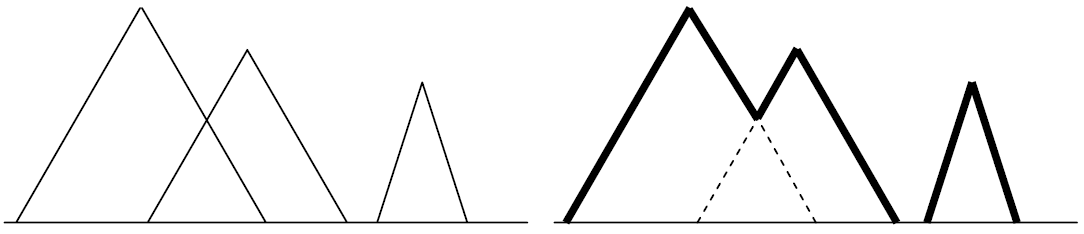
\includegraphics[width=0.9 \textwidth]{2008j.png}
					\caption{山坡与轮廓} \label{2008j}
					\vskip-1em
				\end{figure}
				
				山峰数 $N \le 100$。
			\subsubsection{简要分析}
				对于所有三角形,两两地求出其所有交点。加上端点,设总共有 $M$ 个 点,那么将这些点横坐标排序,就能将整个地面分成 $(M + 1)$ 部分。每一部分里,需要计算的“轮廓”都是直线,由区间端点上最高的处的位置连接而成。求出端点上的高度后,套用勾股定理求轮廓长度之和即可。
				
			\subsubsection{时空复杂度}
				$\mathcal{O}(M) =  \mathcal{O}\left(N^2\right)$,故时间复杂度
				$ \mathcal{O}\left(MN\right) = \mathcal{O}\left(N^3\right)$。
				
				空间复杂度 $\mathcal{O}\left(N^2\right)$。
				
				
		\newpage
			
			
	
	\section{ACM/ICPC World Finals 2007}
		\subsection{ACM/ICPC World Finals 2007 A Consanguine Calculations}
			\subsubsection{题目大意}
			ABO 血型由 $i, I^A, I^B$ 三个等位基因确定。$I^A, I^B, i$ 分别产生 A, B, O 型。$I^A, I^B$ 是显性的,而且是共显性的; $i$ 是隐性的。具体地,等位基因型与 ABO 血型的对应情况见表 \ref{ta1}。
				\begin{table}[!htb]
					\centering
					\begin{tabular}{cccc}
						\toprule
							\multicolumn{2}{c}{等位基因}& & ABO 血型   \\
						\midrule
							$ii$&(OO) && O\\
							$I^Ai$&(AO) && A\\
							$I^AI^A$&(AA) && A\\
							$I^Bi$&(BO) && B\\
							$I^BI^B$&(BB) && B\\
							$I^AI^B$&(AB) && AB\\
						\bottomrule
					\end{tabular}
					\caption{等位基因型- ABO 血型}\label{ta1}
				\end{table}
			
			除了 ABO 血型外,还有 Rh 血型。 Rh 血型根据被测者是否具有 Rh 抗原而划分为阴性和阳性。Rh 抗原繁多,故 Rh 血型系统较为复杂,但 只要被测者控制 Rh 等位基因都为隐性(阴性,-),那么被测者的 Rh 血型就是阴性;否则被测者 Rh 呈阳性。 % 所有基因都是显性的。
				
			给定父母子三人中两人的 ABO 血型 和 Rh 血型,判断第三个人可能的 ABO 血型 和 Rh 血型。
			
		\subsubsection{算法讨论}
			枚举父母的 ABO 等位基因和 Rh 等位基因,判断是否满足给定条件,再根据孟德尔定律判断孩子的等位基因,导出孩子的血型。
			
			取出所有满足条件的情况,去重后作为答案输出。
			
			\subsubsection{时空复杂度}
				时间复杂度 $\mathcal{O}\left(1\right)$。内含常数 $(6 \times 4)^2 \times 2 \times 2 = \num{2304}$。
					
				空间复杂度 $\mathcal{O}\left(1\right)$。
		\newpage

	
		\subsection{ACM/ICPC World Finals 2007 E Collecting Luggage}
			\subsubsection{题目大意}
			如图 \ref{2007e},机场的行李提取轨道为一简单多边形。给定
			行李的起始位置,速度,以及人的起始位置,速度。不跨越轨道,求人拿到行李的最短时间。人的速度快于行李速度。
				\begin{figure}[htb]
					\centering
					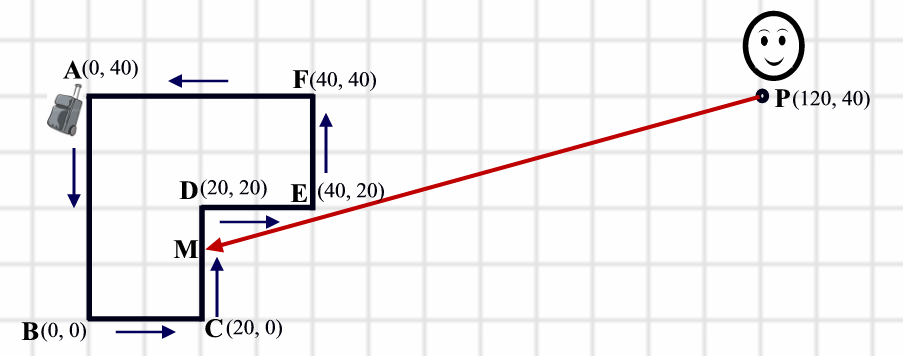
\includegraphics[width=0.7 \textwidth]{2007e.png}
					\caption{行李提取轨道} \label{2007e}
				\end{figure}
			
			行李轨道的顶点数 $N \le 100 $。
		\subsubsection{算法讨论}	
			由于人的速度快于行李速度,故提取到了行李后,也可以磨蹭时间,跟着行李同步走,于是乎答案单调。可以先二分,将问题简化成判定性问题。
			
			设二分的时间 $t_0$,那么需回答 $t = t_0$ 时刻,人能否拿到行李。行李的轨迹是固定的,可以算出其在 $t = t_0$ 时的位置。那么只需确定人能否在  $t = t_0$  时刻赶到行李处;或者说,求出到达该行李处的最短时间,看其是否不超过 $t_0$。
			
			要最快地到达行李在 $t = t_0$ 的位置,可以证明只需在起点,终点,多边形顶点间走直线。此命题较经典,故在此节省篇幅省去证明。枚举两点,判断是否跨越多边形,如果没有跨越,就加边,直到完成建图。最后只需运行 Dijkstra 等最短路算法即可求出最短时间,与 $t_0$ 比较,反馈给二分搜索。
			
			\emph{一些最短路的询问可以预先处理,因为二分算法询问的时间 $t_0$ 不会修改这些信息。}
			
			最终的答案由二分搜索给出。
					
			\subsubsection{时空复杂度}
				由于预处理,时间复杂度 $\mathcal{O}\left(k + N^2\right)$。$k$ 是二分的次数,与精度有关。
					
				空间复杂度 $\mathcal{O}\left(N^2\right)$。
		\newpage
					
	
		\subsection{ACM/ICPC World Finals 2007 F Marble Game}
			\subsubsection{题目大意}
			如图 \ref{2007f},一个 $N \times N$ 的板子上有 $M$ 个球 $M$ 个洞,且一一对应。倾斜板子(上下左右)可使得球滚动。\emph{必须等到球滚动停止,才能更改倾斜方向。球入洞后,会填平空隙。}设计一种方案,倾斜最少的次数,使得球对号入座。
				\begin{figure}[htb]
					\centering
					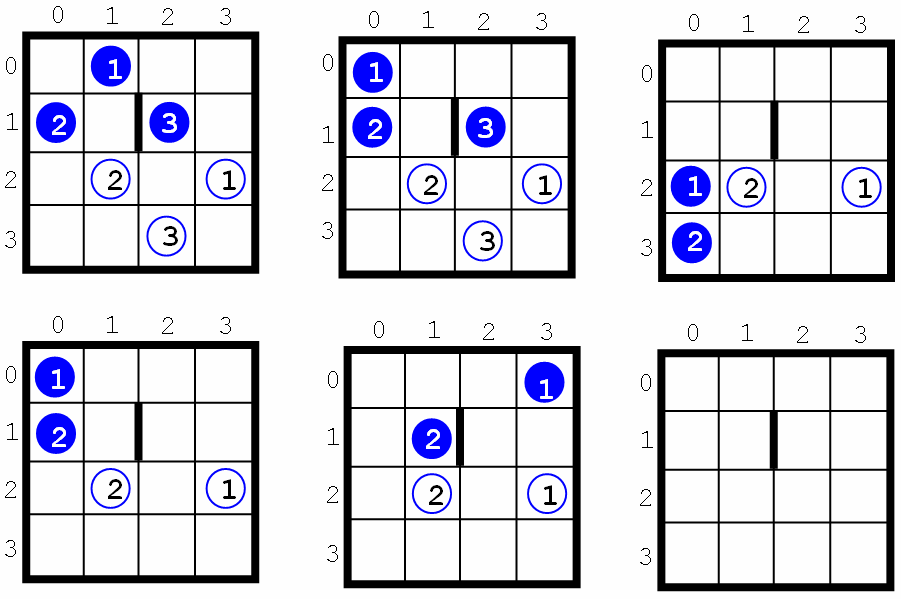
\includegraphics[width=0.7 \textwidth]{2007f.png}
					\caption{} \label{2007f}
				\end{figure}
			
			$N \le 4$。 
			
			\subsubsection{算法讨论}
				直接从起始局面开始 BFS,枚举四个方向,并模拟当前的情况,将搜索出的情况加入队列。
				
				去重可使用 set 等 STL。
				
				情况数的最大值为 $\binom{4 \times 4}{4 \times 4 / 2} = 12870$。
				
			\subsubsection{时空复杂度}
				时间复杂度 $\mathcal{O}\left(N^2f(N) N^2\log f(N)\right)$。 $f(N)$ 表示情况数。题中 $f(N) \le 12870$。
					
				空间复杂度 $\mathcal{O}\left(N^2f(N)\right)$。
				
			
		\newpage
					
	
		\subsection{ACM/ICPC World Finals 2007 H Raising the Roof}
			\subsubsection{题目大意}
				\emph{空间}中有若干三角形,且两两不交(不含边界)。一束平行光从上往下照射,被照到的部分需染色。问总计需染色多大的面积。
				
				三角数 $N \le 1000$,顶点数 $M \le 300$。
			\subsubsection{算法讨论}
				先将空间问题平面化。根据射影定理,如果一个面积为  $S$ 三角形在平面 $\alpha$ 的投影的面积为 $S^\prime$,那么此三角形与平面 $\alpha$ 的二面角 $\theta$ 满足
				\begin{align}
					\cos \theta = \frac{S^\prime}{S} \label{07hhhh}
				\end{align}
				根据 \eqref{07hhhh}, $S = S^\prime / \cos \theta$,故忽略掉高坐标后,相当于一个带权的平面三角面积并,每个三角的权为与 $xOy$ 平面的二面角的倒数  $1/ \cos \theta$。 一个细节是要先删除掉完全竖直的三角形,因为其本身投影到 $xOy$ 平面相当于一条直线,不影响答案,但权值为 $\infty$。
				
				随后考虑这个平面问题。求出所有交点,将纵坐标取出并排序,就可以将整个平面划分为若干横条。可以证明各个横条中要被计算的图形都是梯形(满足线性),故只需对各个横条的中点扫描,乘上横条的粗细,计入答案即可。
				
				注意到我们需要维护处于(空间中)最高点的图形的权值,此处可以用扫描线 + 平衡树。对于横条的中线,每个三角形与其交必然是区间(或者空集),将左端点视为插入,右端点视为删除,以高度来维护三角形集的信息。在相邻事件的中点,需要求到最上的三角形的权值,将其乘上相邻事件的长度,求和并返回即可。
					
			\subsubsection{时空复杂度}
				时间复杂度 $\mathcal{O}\left(N^3\log N\right)$。上限较宽松,程序运行速度还是满意。
					
				空间复杂度 $\mathcal{O}\left(N\right)$。
				
			
			
		\newpage
					
	
		\subsection{ACM/ICPC World Finals 2007 I Water Tanks}
			\subsubsection{题目大意}	
				
				如图 \ref{2007i},有 $N$ 个等粗的水缸,第一个开口,与大气接触,其余的水缸相邻两个间都有一个管道,体积不计,且\emph{高度递增}。问将第一个水缸灌满须多少水。
				
				
				\begin{figure}[htb]
					\centering
					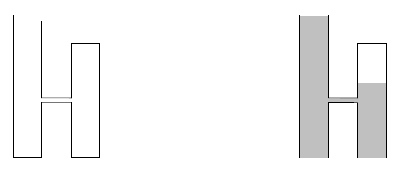
\includegraphics[width=0.7 \textwidth]{2007i.png}
					\caption{水缸灌水前后} \label{2007i}
				\end{figure}	
			
				$N \le 10$。标准大气压 $p_0$,水的密度 $\rho$,重力加速度 $g$%,水缸底面积 $S$,水缸高度 $h_i$ 
				已知
				,玻意耳-马略特定律
				\begin{align}
					p_1 V_1 = p_2 V_2
				\end{align}
			\subsubsection{算法讨论}
				先假设第一个水缸的高度无穷大,%这样
				即我们可以一直灌水。这样整个灌水过程可以描述为
				\begin{enumerate}
					\item 先把第一个水缸灌到管道处,紧接着第二个水缸也被灌到了管道处。
						此时第二个水缸到其后所有水缸的气体封闭。$i = 2$。
					\item 第 $i$ 个水缸因为第一个水缸的水压,致使水面缓缓抬升,气体压缩。如果第一个水缸的液面高度 $h_1$,压缩前 第 $i$ 个水缸到最后一个水缸的气体的压强 $p$,体积 $V$,第 $i$ 个水箱与第 $i - 1$ 个水箱的管道高 $H$
					,这样此水缸的高度 $h_i$ 满足
						\begin{align}
							(\rho g \cdot (h_1 - h_i) + p_0) \cdot (V - S \cdot (h_i - H)) = p V \label{2007i}
						\end{align}
					且从 \eqref{2007i} 中可以看到 $h_1$ 随 $h_i$ 的单调性。如果 $i = n$ ,则此阶段一直进行;否则此阶段直到 $h_i$ 上升到其与 $(i + 1)$ 号水箱间的管道处为止。
					\item $h_i$ 不再变化,水流向 $h_{i+1}$。此时的方程与  \eqref{2007i} 类似:
						\begin{align}
							(\rho g \cdot (h_1 - h_i) + p_0) \cdot (V - S \cdot (h_i - h_{i+1} - H)) = p V \label{2007i2}
						\end{align}
						$h_1$ 随 $h_i$ 单调。此过程直到 $h_{i+1}$ 上升到 $i$ 号水箱与 $(i + 1)$ 号水箱间的管道处为止。
						此时 第 $i$ 个水箱 的气体单独封闭,此部分的气体质量不会再变化。\emph{令 $i$ 自增一},则第 $i$ 个水缸到其后所有水缸的气体再次封闭。跳到步骤 2。
				\end{enumerate}
				
				如果按照此步骤一直进行下去,$h_1$ 将会 $\to + \infty$。而 $h_1$ 只需上升到某一特定值即可退出程序,故某一阶段可能会执行到一半就会中断退出。不过没关系,确定了退出时的 $h_1$ 就可以根据  \eqref{2007i} \eqref{2007i2} 解出对应的 $h_{i, i+1}$,二分或者数学方法皆可。最后用 玻意耳-马略特定律 更新一下单独封闭掉的气体体积,求个和,从水箱总体积里扣去就是答案。
			
			\subsubsection{时空复杂度}
				时间复杂度 $\mathcal{O}\left(N k\right)$。$k$ 是解方程是二分的次数,与精度相关。
					
				空间复杂度 $\mathcal{O}\left(N\right)$。
				
		\newpage
					
	
		\subsection{ACM/ICPC World Finals 2007 J Tunnels}
			\subsubsection{题目大意}
				有向图 $G = (V, E)$。一个人从 $s \in V$ 开始走,$t \in V$ 是终点。你可以随时监控他的位置,并每次在其到达某一节点后,就可以删除某些边。问至少删除多少条边,才能使得其无法到达终点。
				
				$N = |V| \le 50, M = |E| \le 100 $。
			\subsubsection{算法讨论}
				此问题看起来像是最小割问题——将 $s, t$ 割开,使其不连通。但是仔细分析下就会发现这个问题并没有这么简单,因为可以监控其行走的轨迹,故可以在其行动之后,根据其选择再进一步决定删边的方案。
				
				为了解决这一问题,我们对于每个点 $v \in V \setminus \{ t\}$,定义一个变量 $F(v)$,使得其最终将会变成此人从 $v$ 开始走的情况下,保证不到达 $t$ 最少须删除的边数。
				
				初步的算法流程如算法 \ref{2007jalgo}。%下
				\begin{algorithm}[H]
				\caption{求出正确的 $F(x)$}
				\label{2007jalgo}
					\begin{algorithmic}[1]
						\State $F(\cdot) \gets + \infty$
						\For{如果此人在 $u$ 点,删掉 $x$ 条边后,必须经过 $F(v)$ 值 $\le y$ 的点 $v$才能出去}  \label{2007jaaa}
							\If{$F(u) > x + y$}
							\State $F(u) \gets x + y$
							\EndIf
						\EndFor
					\end{algorithmic}
				\end{algorithm}
				\begin{algorithm}[tbh]
				\caption{求出正确的 $F(x)$ ver. 2.0}
				\label{2007jalgo2}
					\begin{algorithmic}[1]
						\For{$u \in V \setminus \{ t\}$}
							\State $F(u) \gets \Call{MinCut}{u, t}$
						\EndFor
						\State 设置所有 $v \in V \setminus \{ t\}$ 为未访问的点
						\For{还剩下未访问的点} 
							\State $Min \gets \min_{\text{未访问过的}\, x}{F(x)}$
%							\If {$Min = +\infty$}
%								\State \textbf{break}
%							\EndIf
							\State 访问所有满足 $F(v) = Min$ 的 $v$,并在图 $G = (V, E)$ 中删除它们 \Comment{$F$ 值已经固定。}
							\For{未访问过的  $x$ } 									 \Comment{更新$(y = Min)$。}
								\If{$F(x) > \Call{MinCut}{x, t} + Min$}
								\State $F(x) \gets \Call{MinCut}{x, t} + Min$
								\EndIf
							\EndFor
						\EndFor
					\end{algorithmic}
				\end{algorithm}
				
				我们稍后将会证明算法 \ref{2007jalgo} 第  \ref{2007jaaa} 行中找 $(u, x, y)$ 的顺序不会影响答案,以及算法 \ref{2007jalgo} 的正确性。
				
				进一步观察,发现 一旦确定了 $u, y$ 的值后,可将所有的  $F(v)$ 值 $\le y$ 的点 $v$ 删去,求最小割,即可求到最小的 $x$ 值。
				而所有的 $f(\cdot)$ 都在不断下降,故只有较小的 $f(\cdot)$ 才能够更新较大的 $f(\cdot)$。不妨从小往大确定 $f(\cdot)$ 的正确值。进一步优化后可得出算法 \ref{2007jalgo2}。此算法能在 $\mathcal{O}\left( N^2MaxFlow(N, M) \right)$ 的时间复杂度内出解。$Maxflow(N, M)$ 是求解 $N$ 个点 $M$ 条边的网络流的时间。
				
				以下是此算法的正确性证明。
				\begin{theorem} \label{2007jaaaaa}
						算法 \ref{2007jalgo} 第  \ref{2007jaaa} 行中找 $(u, x, y)$ 的顺序不会影响答案。
				\end{theorem}
				\begin{pf}
					算法执行过程中,$G = (V, E)$ 不会变化,$F(\cdot)$ 单调下降,故若某一时刻起,  $(u, x, y)$  是算法  \ref{2007jalgo} 第  \ref{2007jaaa} 行要寻找的项(下称“可行优化”),那么他将一直成为可行优化,直到其被处理为止。\qed
				\end{pf}
				\begin{theorem}
						算法 \ref{2007jalgo} 提供的 $F(s)$ 值是足够的。
				\end{theorem}
				\begin{pf}
					如果最后一次更新 $F(s)$ 的操作是 $(s, x, y)$,那么我们可以删掉 $x$ 条边,把它逼到一个 $F(s^\prime) \le y$ 的点 $s^\prime$,然后继续下去,这一步不会超过 $F(s^\prime)$ 次删除(归纳),在加上前面的 $x$ 次删除,故总计 $F(s)$ 次删除足矣。\qed
				\end{pf}
				\begin{lemma}
						设图 $G = (V, E), G^\prime = (V, E \setminus \{e\})$,$G$ 中 $x$ 点的 $F(x)$ 值为 $F_1(x)$,$G^\prime$ 中 $x$ 点的 $F(x)$ 值为 $F_2(x)$,则 $\forall x \in V, F_1(x) - 1 \le F_2(x)  \le F_1(x)$。
						\label{2007jlemma}
				\end{lemma}
				\begin{pf}
					因为 $G$ 比 $G^\prime$ 多一条边,故所有能在 $G$ 中执行的可行优化 $(u, x, y)$ 在 $G^\prime$ 中肯定能实施,故  $\forall x \in V, F_1(x)\ge F_2(x)  $。
					
					根据定理 \ref{2007jaaaaa},可以假设一开始算法将 $G^\prime$ 的 $F(\cdot)$ 值被优化成了跟 $G$ 最终一模一样的情况$(F_1(x) = F_2(x))$。不是一般性,我们可以假设此算法每次都对 $F_2(\cdot)$ 减少 1。
					下说明,接下来同一个点 $u$ 的 $F_2(u)$ 不会被优化两次。
					
					先考虑第一次 $F_2(u)$ 被 $(u, x, y)$ 优化的情况。由于其不适用于 $G$,故有以下可能
						\begin{enumerate} 
							\item 在 $G^\prime$ 中删掉这 $x$ 条边后,有一条到达终点的路径不经过一个 $F_1$ 值 $\le y$ 的点,而其经过了一个 $F_2$ 值 $\le y$ 的点 $v$。此处应假设还暂时没有点的 $F_2$ 值被优化两次,故 $F_2(v)$ 已经被优化过了,$F_2(v) = y$,$G$ 中 $F_1(v) = y + 1$,而需注意 $F_2(u) = x + y \ge x = F_2(v) $。
							\item  在  $G^\prime$ 中删掉这 $x$ 条边后,所有到达终点的路径都会经过一个 $F_1$ 值 $\le y$ 的点,而其不能对 $F_1(u)$ 优化显然是因为 $G$ 中多了一条原先被删除的边 $e$ 后,给了 $u$ 到终点的一条不经过  $F_1$ 值 $\le y$  的点的路径。于是乎, $(u, x + 1, y)$ 才适用于 $F_1(u)$。这样,必然存在一条 $u$ 到 $e$ 的一个端点 $e_0$ 的路径,其不经过任何一个  $F_1$ 值 $\le y$ 的点 。否则的话所有经过  $e$ 到达终点的路径都会经过一个 $F_1$ 值 $\le y$ 的点,致使 $(u, x, y)$ 适用于优化 $F_1(u)$,从而造成矛盾。因此,$(e_0, x + 1, y)$ 也适用于 $F_1(e_0)$,因为删掉这 $x$ 条边和 $e$ 后,就不会有不经过 $F_1$ 值 $\le y$ 的点到达终点的路径,因为如果不是这样,那么可以利用刚才的提到的路径,结合不经过 $F_1$ 值 $\le y$ 的点从 $e_0$ 到达终点的路径,将其延伸成一条不经过 $F_1$ 值 $\le y$ 的点从 $u$ 到终点的路径,与 $(u, x, y)$ 不适用于 $F_1(u)$ 造成矛盾,于是乎,$F_1(e_0) \le x + y + 1 = F_2(u) + 1$。
						\end{enumerate}
						
						综上,可以说明对于任意优化了的  $F_2(u)$, $F_1(e_0) \le F_2(u) + 1$。
						接下来,考虑第二次 $F_2(u)$ 被 $(u, x, y)$ 优化的情况。由于其还是不适用于 $G$,故仍有以下可能
						\begin{enumerate} 
							\item 在 $G^\prime$ 中删掉这 $x$ 条边后,有一条到达终点的路径不经过一个 $F_1$ 值 $\le y$ 的点,而其经过了一个 $F_2$ 值 $\le y$ 的点 $v$。与前面的同理,必然有一个 $F_2(v)$ 从 $y + 1$ 减少到了 $y$。根据前面的判断, $F_1(e_0) \le y + 1$。故  $(u, x, y + 1)$ 是适用于 $F_2(u)$ 的:不使用 $e$ 的必然跨过一个 $F_1$ 值 $\le y + 1$ 的,(因为目前应假设还暂时没有点的 $F_2$ 值被优化两次)也就是 $F_2$ 值 $\le y$,这是满足我们的假设的;而适用 $e$ 的必然经过 $e_0$, $F_1(e_0) \le y + 1$。这样 $F_1(u) = x + y + 1, F_2(u) = x + y$,与其为第二次优化是互相矛盾的。
							\item 在  $G^\prime$ 中删掉这 $x$ 条边后,所有到达终点的路径都会经过一个 $F_1$ 值 $\le y$ 的点。这样  $(u, x + 1, y)$ 是适用于 $F_2(u)$ 的:删掉 $e_0$ 和这 $x$ 条边,变成与 $G^\prime$ 相似的情况。这样 $F_1(u) = x + y + 1, F_2(u) = x + y$,与其为第二次优化是互相矛盾的。
						\end{enumerate}
					
					综上,只能每个 $F_2(x)$ 优化一次并减少 $1$,引理得证。 \qed

				\end{pf}
				
				\begin{theorem}
						算法 \ref{2007jalgo} 提供的 $F(s)$ 值是必要的。
				\end{theorem}
				\begin{pf}
					设我们只有 $F(s) - 1$ 次删边操作,那么此人会寻找一条通往终点,不经过 $F$ 值低于 $F(s)$ 的路径(否则可以进行 $(s, 0, y), y < F(s)$ 的优化,与条件矛盾),直到我们进行了一次删边操作。删边前,此人所在点的 $F$ 值 $ \ge F(s)$,根据引理 \ref{2007jlemma},删边后,此人所在点的 $F$ 值 $ \ge F(s) - 1$,而我们还剩下 $F(s) - 2$ 次删边操作。重复迭代上述操作,当此人所在点的 $F$ 值 $ \ge 1$ 时,我们就不能再删边了,这样它就可以直接走向出口了 
%					{\rm
%					( ̄\hskip-0.05em$\bigtriangledown$\hskip-0.05em ̄ ") 
%					(" ̄$ \bigtriangledown $ ̄)/}
					。
					故 $F(s) - 1$ 次删边是不足的。\qed
				\end{pf}
				至此,本算法的所有正确性说明完毕。
			\subsubsection{时空复杂度}
				时间复杂度 $\mathcal{O}\left( N^2 MaxFlow(N, M)\right)$。$Maxflow(N, M)$ 是求解 $N$ 个点 $M$ 条边的网络流的时间。
					
				空间复杂度 $\mathcal{O}\left(N + M\right)$。
				
		\newpage
					
				
	
	\section{ACM/ICPC World Finals 2006}
		\subsection{ACM/ICPC World Finals 2006 A Low Cost Air Travel}
			\subsubsection{题目大意}
				有 $N$ 个机票套餐,每张机票套餐是连续的若干转乘机票。第 $i$ 个套餐经过 $n_i$ 个站点
				\begin{align}	
					p_{i,1} \rightarrow p_{i,2} \rightarrow p_{i,3}  \rightarrow \cdots \rightarrow p_{i, n_i}
				\end{align}
				售价 $w_i$ 元,剩余无数张。每张票必须从头开始乘坐,也就是说如果乘客没有乘坐 $p_{i,j} \rightarrow p_{i, j + 1}$,那么就不能乘坐 $ p_{i, j + 1} \rightarrow p_{i, j + 2}$。同时,乘坐 $p_{i,j}\rightarrow p_{i , j+ 1}$ 到达 $p_{i, j + 1}$ 后乘坐其他飞机,最后又回到 $p_{i, j + 1}$,再乘坐 $ p_{i, j + 1} \rightarrow p_{i , j + 2}$ 也是不允许的。今有一个 $M$ 旅行计划
				\begin{align}	
					q_{i,1} \rightarrow q_{i,2} \rightarrow q_{i,3}  \rightarrow \cdots \rightarrow q_{i, K_i} \label{2006a1}
				\end{align}
				问需要买多少机票才能完成此计划,并给出具体乘坐的方案。
				
				$N \le 20, M \le 20, K_i \le 10, n_i \le 10$。
			\subsubsection{算法讨论}
				动态规划。设 $F[i][j][k]$ 表示 已经游览了\eqref{2006a1} 中的前 $i$ 个城市,现在在套餐 $j$ 的第 $k$ 个中转站。转移
				\begin{align}
					F[i][j][k] & = \begin{cases}
						F[i^\prime][j][k - 1], & k > 1\\
						w_j + \min_{j^\prime, k^\prime}  F[i][j^\prime][k^\prime], & k = 1, p_{j, k} = p_{j^\prime, k^\prime}
					\end{cases}
					\intertext{其中}
					i^\prime&  = \begin{cases}
						i - 1, &p_{j, k} = q_{\text{当前旅行计划}, i}\\
						i, &\text{其他}
					\end{cases}
				\end{align}
				转移可能需最短路算法来实现。
				答案 $\min F[K_i][\cdot][\cdot]$。记录下转移即可输出方案。
				
				由于有 $M$ 个计划,故上述算法需执行 $M$ 次。
			
			\subsubsection{时空复杂度}
				时间复杂度 $\mathcal{O}\left(\sum_j K_j \cdot \sum_i n_i \log K_j \cdot \sum_i n_i \right)$。题中 $\sum_j K_j \cdot \sum_i n_i \log K_j \cdot \sum_i n_i  \le 20 \times \num{2000} \log \num{2000}$
					
				空间复杂度 $\mathcal{O}\left( \max_j K_j \cdot \sum_i n_i\right)$。

		\newpage
		\subsection{ACM/ICPC World Finals 2006 B Remember the A La Mode!}
			\subsubsection{题目大意}
				给定整数 $a_i, b_j, w_{i, j} (1 \le i, j \le N)$,解整数线性规划
				\begin{align}
					\text{maximize/minimize} & \sum_{i,j} w_{i,j}x_{i,j}   \label{2006bb} \\
					\text{s.t.} & \begin{cases}
						\sum_{j} x_{i, j} = a_i\\
						\sum_{i} x_{i, j} = b_j\\
								x_{i, j} \ge 0\\
								x_{i, j} \in \mathbb{Z}
					\end{cases} \label{2006b}
				\end{align}
				
				$N \le 50$。
			\subsubsection{算法讨论}
				可根据 \eqref{2006bb} \eqref{2006b} 建图,运行最大(小)费用网络流,求出答案。
			\subsubsection{时空复杂度}
				
				时间复杂度 $\mathcal{O}\left(Maxflow(2N+2, 2N+N^2)\right)$。$Maxflow(N, M)$ 表示计算 $N$ 个点 $M$ 条边的最优费用流的复杂度。
					
				空间复杂度 $\mathcal{O}\left(N^2\right)$。
			
		\newpage
		\subsection{ACM/ICPC World Finals 2006 C Ars Longa}
			\subsubsection{题目大意}
				空间中有 $N$ 个相同的塑料球,用 $M$ 个不可伸缩的棒连接。给定这些球的位置,以及 $M$ 根木棒的连接情况。$z = 0$ 是地面,且在地面上的球都粘贴在地面上,其余则满足 $z > 0$。问这个系统是否静止;如果静止,是否稳定(受到足够小的外力后仍然静止)。
				
				$N, M \le 100$。
			\subsubsection{算法讨论}
				要静止,则必须要使得塑料球均静止。$z = 0$ 上的球粘贴在该平面上,肯定静止,无需考虑。
				
				显然,每个物体受重力 $\mathbf{G} = -G \mathbf{k}$。对于木棒,根据刚体力学,其可受拉力和压力,不妨假设其受大小 $F$ 的拉力(压力则取负),连接的两球位置向量 $\mathbf{p, q} $,则 $p$ 受拉力 
				\begin{align}
					\mathbf{F}_p & = F \frac{\mathbf{q} - \mathbf{p}}{  \left|\mathbf{q} - \mathbf{p} \right|}
					\intertext{$q$ 受拉力 }
					\mathbf{F}_q & = F \frac{\mathbf{p} - \mathbf{q}}{  \left|\mathbf{p} - \mathbf{q} \right|}
				\end{align}
				只需要每个 $z > 0$ 的球重力和木棒的拉力加起来为 $\mathbf{0}$ 即可,这样就构成了 $N^\prime$ 个方程 $M$ 个未知数的线性方程组,$N^\prime$ 是未处于地面的小球数量,$M$ 个木棒拉力大小 $F_i$ 未知,为未知数。运行高斯消元解这个方程组就可以知道其是否静止。
				
				而要检查其是否稳定,只需检查系数矩阵的秩是否为  $N^\prime$ 。因为如果不为  $N^\prime$,那么运行高斯消元后,会有若干形如
				\begin{align}
					(0, 0, \ldots, 0) \cdot (F_1, F_2, \ldots, F_M) = 0 \label{2006c}
				\end{align} 的式子。这样肯定存在某个方向的微小外力,使得 \eqref{2006c} 的常数项变成一个微小的非零值 $\epsilon$,导致整个方程无解,系统不静止。反正如果秩恰为 $N^\prime$ 那么不管常数在外力下如何变化,根据线性代数,肯定能用高斯消元求出一组解。如果 
				秩恰为 $N^\prime$,$M = N^\prime$,那么将会仅有一组可行解。
			\subsubsection{时空复杂度}
				
				时间复杂度 $\mathcal{O}\left(N^2M\right)$。
					
				空间复杂度 $\mathcal{O}\left(NM\right)$。
			
		\newpage
		\subsection{ACM/ICPC World Finals 2006 D Bipartite Numbers}
			\subsubsection{题目大意}
				定义二次重复数 $(a,b,n,m) = (\underbrace{aaa\cdots a}_{n \text{ 个} \, a}
				\underbrace{bbb\cdots b}_{m \text{ 个} \, b})_{10}, 0 < a \le 9, 0 \le b \le 9, n,m > 0$。
				
				对于一个 $x$,求一个最小的 $y$,使得 $x | y$,且 $y$ 是二次重复数,并输出其 $a, b, n, m$。
				
				$1 \le x \le \num{99999}$,多组询问。
			\subsubsection{算法讨论}
				预处理 $F(i) = 10^i \mod{x}$ 和 $G(i) = (10^i - 1) / 9 \mod{x}$,两者都可以用递推处理,转移方程 $F(i) = 10 \,F(i - 1) \mod{x}, G(i) = (10\,G(i-1) + 1) \mod{x}$。
				
				这样二次重复数 $(a,b,n,m)$ 能被 $x$ 整除当且仅当 
				\begin{align}
					a\,G(n)\,F(m) +  b\,G(m) \equiv 0 \pmod{x} \label{2006d}
				\end{align}
				
				先从小到大枚举 $n+m$ 再枚举 $n, m, a, b$ 使用 \eqref{2006d} 判断即可求到最小值。
				
				实践之后会发现,对于非整十的值 $x$,上述算法效率非常高;但是如果是整十的,那么由于其后几位不管翻几倍都是 0。要形成二段数,前面的必然是一连串相同的数,而实践可知,这样的 $n$ 异常庞大, $m$ 却非常非常小。如果按照上述算法的步骤进行爆搜,耗时非常多。
				
				 针对整十的数 $x, 1 \le x \le \num{99999}$,通过爆搜可以发现,不存在满足
					\begin{align}
						n + m > 30, m > 20\label{2006dddd}
					\end{align}
				的最优解。这样我们可以使用 \eqref{2006dddd} 作为减枝,加快搜索速度,达到满意的效果。
				
				 
			\subsubsection{时空复杂度}
				
				时间复杂度难以分析,但由于我们的算法用到了 $1 \le x \le \num{99999}$ 这个条件,这样这个算法能解决的问题的上限就固定了,故应算作常数 $\mathcal{O}\left(1\right)$。但从应用的角度看,经过如上的优化后,程序运行的速度能够接受。
					
				空间复杂度 $\mathcal{O}\left(1\right)$。
			
		\newpage
		\subsection{ACM/ICPC World Finals 2006 E Bit Compressor}
			\subsubsection{题目大意}
				一个长度为 $N$ 的零一串,如果将连续的 1 (前后均为 0 或者位于串的两端)取出,用 1 的长度(二进制)来替换后,能缩短这个串 的长度,那么就替换掉它。
				
				已知此串用上述方法压缩成了 长度为 $M$ 的已知串。请问原串是否存在;如果存在,是否有多可可能的原串。
				
				$M \le 40, N \le \num{131072}$。
			\subsubsection{算法讨论}
				暴力搜索。压缩后的部分其两端有 0(或位于整个串的两端),以 1 开头,且不可能是 $10$,因为 $11$ 不可能压缩成 $10$,原因是长度没有变化。$10, 1$ 两个串压缩前后都是一样的,不必判断。
				
				而 0 需要枚举其究竟是原始的,还是作为压缩数据存在的。
				
				整个枚举的过程就像是对长度为 $N$ 的串划分。
				
				一旦搜到两个合法解就立即退出。
			\subsubsection{时空复杂度}
				时间复杂度涉及到一个组合问题,不便于求出。但考虑到 $M \le 40$,加上本题的限制,暴力搜索还是能够胜任。
				
				空间复杂度 $\mathcal{O}\left(M\right)$。

		\newpage
		\subsection{ACM/ICPC World Finals 2006 F Building a Clock}
			\subsubsection{题目大意}
				有一个电动轴。有 $N$ 个齿轮数已知的齿轮和若干轮轴。给定电动轴的角速度,请通过这个轴,以及若干咬合的齿轮,拼接出一个角速度 \SI{1}{r\per\hour} 和角速度 \SI{2}{r\per\day}  的齿轮。齿轮固定在轴上。一个角速度 $r_1$ 齿轮数 $T_1$ 的齿轮与角速度 $r_2$ 齿轮数 $T_2$ 的齿轮咬合后,满足
				\begin{align}
					r_1\,T_1 + r_2T_2 = 0\label{2006f}
				\end{align}
				输出轴使用最少的,其次齿轮使用最少的,最后按题目输出的字典序最少的。
				
				$3 \le N \le 6$
			\subsubsection{算法讨论}
				这个齿轮系统就像是一个树。使用同一个轴串起来的就是兄弟,其有相同的角速度;咬合起来的齿轮就是一对父子,角速度的值根据 \eqref{2006f} 推知。将电动轴抽象成一个点,则其为根。
				
				使用 DFS 算法可以搜索出所有合法的拼接方法(树),再按照题目的规定,取字典序最优的输出。

			\subsubsection{时空复杂度}
				时间复杂度涉及到一个组合问题,不便于求出。但考虑到 $N \le 6$,加上本题的限制,暴力搜索肯定能够胜任。
				
				空间复杂度 $\mathcal{O}\left(N\right)$。
			
		\newpage
		\subsection{ACM/ICPC World Finals 2006 G Pilgrimage}
			\subsubsection{题目大意}
				某人管理一个旅行团(他自己也算在内)的钱。每当有新的人进入时,他会要求每个新人交纳目前每人平均已交纳的钱;同时,如有人退出,他则按照每人平均已交纳的钱退还。可能地,他还会同时向大家各收取相同的一笔整数金额的钱;或者,以集体的名义消费某金额的钱。整个过程中没有出现小数,管理钱的人一直都在该旅游团里。给定这些事件,问最开始的时候可能有多少人?
				
				\emph{最开始时集体的钱数未知。}
				
				事件数 $M \le 50$,每次消费的金额上限 $K \le \num{2000}$。
			\subsubsection{算法讨论}
				由于我们只关心整个过程是否产生整数,而不关心团体的钱是否充足,故向大家收取一笔整数数额的钱是我们所不需要关心的,可先忽略(删除)。
				
				为便于接下来的处理,可先将时间上相邻的操作合并,这样相邻的事件类型都不相同,而且不会影响答案。
%				整个时间轴上相邻的操作都
				
				消费事件发生后不会立即平分金钱,故这一阶段原则上不必考虑产生整数的问题。\emph{但}下一阶段必然是入团(退团)的操作,故还是需要求出整个消费的金额的因数,确定人数。
				
				发生入团和退团事件后,需记录当前的人数与开始的偏移,方能继续操作。
				
				整个过程至少都会有一个人,故答案有一个下界,低于此下界的答案要剔除掉。
				
				如果一次消费事件都未发生,则答案为下界到无穷大的区间。
				
				\emph{一开始的总金额未知,故第一次入团和退团事件发生前的消费事件不必处理。}
			\subsubsection{时空复杂度}
				
				时间复杂度 $\mathcal{O}\left(N\sqrt{NK}\right)$。
					
				空间复杂度 $\mathcal{O}\left(NK\right)$。
		\newpage
		\subsection{ACM/ICPC World Finals 2006 I Degrees of Separation}
			\subsubsection{题目大意}
				给定有向图 $G = (V, E)$,设 $u, v$ 的最短路为 $d(u, v)$,则图的连通度为 $Ans = \max_{u, v} d(u, v)$。求 $G$ 的图连通度。
				
				$N = |V| \le 50$。
			\subsubsection{算法讨论}
				对图 $G$ 运行 Floyd-Warshall 算法即可求到 任意 $u, v$ 的 $d(u, v)$。最后根据定义可直接计算连通度,求出答案。
			\subsubsection{时空复杂度}
				
				时间复杂度 $\mathcal{O}\left(N^3\right)$。
					
				空间复杂度 $\mathcal{O}\left(N^2\right)$。
		\newpage
		\subsection{ACM/ICPC World Finals 2006 J Routing}
			\subsubsection{题目大意}
				给定无向图 $G = (V, E)$ 和起点终点 $s, t \in V$。求路径 $s \rightarrow t, t \rightarrow s$,使得其并集所经过的不重复的结点总数最小。
				
				$N = |V| \le 100%, |E| \le 100
				$。
				
			\subsubsection{算法讨论}
				如果不考虑结点的重复计数问题,那么答案为 $s \rightarrow t$ 的最短路长度加 $t \rightarrow s$ 的最短路长度。
				
				如果有重复点,那么两条路径经过重复的点的顺序不一定是互为正逆的关系。也就是说,需要注意到其还可能是以一条重复的路径存在的。如
				\begin{align}
						s \rightarrow A \rightarrow B \rightarrow C \rightarrow D \rightarrow E  \rightarrow t  \\
						t \rightarrow E \rightarrow B \rightarrow C \rightarrow D \rightarrow A \rightarrow s
				\end{align}
				此处 $B, C, D$ 三点就是以一条路径参与去重的。
				
				不妨考虑动态规划。如果 $f[u][v]$ 表示 $s \rightarrow u, v \rightarrow s$ 两条路径共同经过的点数的下限。预处理好 $u, v$ 两点间最短路 $d(u, v)$,按照算法 \ref{2006j} 进行操作。

				\begin{algorithm}[H]
				\caption{计算 $f[u][v]$}
				\label{2006j}
					\begin{algorithmic}[1]
						\State $f[s][s] \gets 1$
						\For{选一个未访问的最小的 $F[x][y]$,并标记访问它} \label{2006jjjj}
								\State 选一个 $z, (x, z) \in E$,执行 $F[z][y] \gets \min(F[z][y], F[x][y] + [z \ne y])$
								\State 选一个 $z, (z, y) \in E$,执行 $F[x][z] \gets \min(F[x][z], F[x][y] + [z \ne x])$ \Comment{延长一个点}
								\State 若 $x \ne y$,则执行 $F[y][x] \gets \min(F[y][x], F[x][y] + d(x, y) - 1$ \Comment{延长一个重复的路径}
						\EndFor
					\end{algorithmic}
				\end{algorithm}
				
				算法 \ref{2006j} 的第 \ref{2006jjjj} 行可用堆实现。答案 $F[t][t]$。

			\subsubsection{时空复杂度}
				
				时间复杂度 $\mathcal{O}\left(N^2\log N\right)$。
					
				空间复杂度 $\mathcal{O}\left(N^2\right)$。
		\newpage
	
	\section{ACM/ICPC World Finals 2005}
		\subsection{ACM/ICPC World Finals 2005 B Simplified GSM Network}
			\subsubsection{题目大意}
				如图 \ref{2005b},有若干基站与城市。城市之间有笔直的道路。问城市 $u$ 沿道路 到 城市 $v$,手机最少要切换几次基站?手机总寻找最近的基站。
				\begin{figure}[htb]
					\centering
					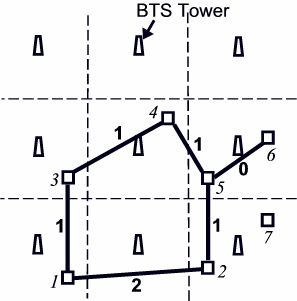
\includegraphics[width=0.3 \textwidth]{2005b.png}
					\caption{基站为梯形,城市为方形} \label{2005b}
				\end{figure}

				基站数 $N \le 50$, 城市数  $M \le 50$,道路数 $K \le 250$, 询问数  $Q \le 10$。道路不会与基站服务范围重合成一条线段。
			\subsubsection{算法讨论}
				根据计算几何,可在
%				先
				求出基站的 Voronoi 图后,与道路求交,将相交次数作为边权,带回原问题,即可用最短路算法求知答案。
				
				但是,求  Voronoi 图 的算法十分复杂,而我们可以避开它 ,不直接求出 Voronoi 图,将  Voronoi 图与道路相交的次数求出。
				
				 Voronoi 图 中所有的线段都是两点的中垂线,故我们先枚举两个基站,求出其中垂线,与道路求交,可能会得到一个交点。如果确实得到了此交点,那么还需判断其是否在 Voronoi 图 上(因为可能在 Voronoi 图 中 这条线段的延长线上),方法是求出这点与其他基站的最短距离,判断这个距离是否为该点到这两个选择的基站的距离。如果不是,那么这个点仍需排除;否则,这个点就是 Voronoi 图与道路的交,权值自增一。
				
				求出边权后,使用最短路算法即可。
			\subsubsection{时空复杂度}
				时间复杂度 $\mathcal{O}\left(N^2K + M^3 + K\right)$。
					
				空间复杂度 $\mathcal{O}\left(N + M^2)\right)$。
		\newpage
		\subsection{ACM/ICPC World Finals 2005 C The Traveling Judges Problem}
			\subsubsection{题目大意}
				给定无向图 $G=(V, E)$,边权 $W: E \mapsto \mathbb{R}^{+}$ ,有 $N_0$ 个人,分别位于 $s_1, s_2, \ldots, s_{N_0}\in V$,均前往同一目的地 $t \in V$。他们可以打无数个的,每个的可容纳无数人,且仅以路程(边权之和)正比例地计费
%				,无起步价,燃油,保险,空程,多人等的收费
				。问他们需要多少钱就可以共同到达目的地?并输出方案。
				
				$N = |V| \le 20, N_0 \le 10
%				, M = |E| \le
				$。
			\subsubsection{算法讨论}
				不妨将他们经过的点标记出来,将其他的点剔除,求最小生成树。可以说明最小生成树的权值就是答案。因为他们都经过了这些点,而进一步缩小答案就会导致图不连通,与假设矛盾;而就以 $t$ 为根,只要这些人都往父亲结点方形走,并在每一条边都与要经过这条边的人和打一辆的即可,答案是足够的。
				
				枚举 $2^N$ 种情况求最小生成树判断即可。记录下最优解的最小生成树就可以输出方案了。
			\subsubsection{时空复杂度}
				时间复杂度 $\mathcal{O}\left(N^2\log N + 2^N \cdot N^2 \right)$。
					
				空间复杂度 $\mathcal{O}\left(N^2\right)$。
		\newpage
		\subsection{ACM/ICPC World Finals 2005 D cNteSahruPfefrlefe}
			\subsubsection{题目大意}
				设有一碟扑克牌  $a_1, a_2, \ldots, a_N$, $N$ 是扑克牌的总张数。一个完美的洗牌是指将这个序列变成
				\begin{align}
					a_{27},  a_1, a_{28}, a_2, \ldots, a_N, a_{N-1}  \label{2005d}
				\end{align}
				一次不完美的洗牌 
				是指形成 \eqref{2005d} 中相邻两项被交换后的结果。
				
				一开始的牌是整齐的 , $a_i = i$。某人连续洗了\emph{不超过} $K$ 次牌,每次都只是完美的或不完美的。给出洗完牌
%				都
				的结果,问每一次洗牌中那些是不完美的,并指出不完美的洗牌中,哪两张牌被交换了。
				
				$N = 52, K = 10$。
			\subsubsection{算法讨论}
				如果直接对次问题建立数学模型,可以发现就是若干置换(完美洗牌),插入一些两个元素的置换(不完美洗牌的交换),使得形成目标置换。经过化简后就可得知,问题就是选择若干只有两个元素的置换相乘,使得形成一个目标置换。简单的说,给定一排打乱的元素,交换不超过 $K$ 次,每次换两个元素,请将其交换成	
%				一个
				一排有序的元素。
				
				由于 $K = 10$,那么可以先枚举此人真正交换元素的次数 $K_0$,再爆搜(迭代加深),每次有 $\binom{52}{2}$ 种交换方法,故总情况数 $\binom{52}{2}^{K_0}$。存在一个减枝,如果目前仅剩余 $x$ 次交换,但有多于 $2x$ 的元素没有回到正确的位置,这时肯定无解,可直接返回。
			\subsubsection{时空复杂度}
				时间复杂度 $\mathcal{O}\left(\binom{N}{2}^K \right)$。
					
				空间复杂度 $\mathcal{O}\left(N\right)$。
		\newpage
		\subsection{ACM/ICPC World Finals 2005 E Lots of Sunlight}
			\subsubsection{题目大意}
				如图 \ref{2005e},给出若干栋楼房的位置,且均位于同一个东西方向的竖直平面。给定当天日出日落的时间,太阳以某一常角速度运动,阳光视为平行光。问其中一些房间那些时刻有阳光照射(某一侧窗完全被照到)?
				\begin{figure}[htb]
					\centering
					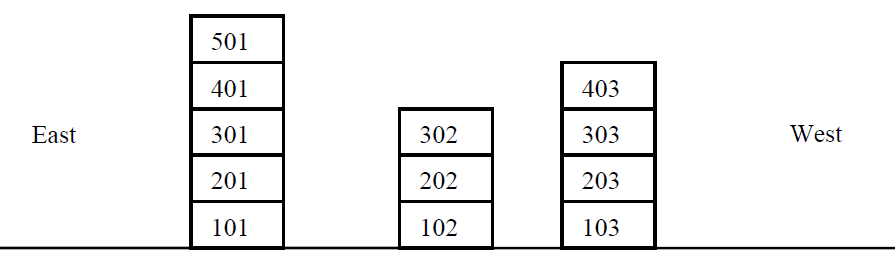
\includegraphics[width=0.7 \textwidth]{2005e.png}
					\caption{} \label{2005e}
				\end{figure}
				
				建筑 $N < 100$
%				,询问数 $M \le $
				。
			\subsubsection{算法讨论}
				求出要询问的房间所在的建筑编号。枚举比这栋楼高的其他建筑,确定该房间的阳光被这栋枚举的楼挡住的临界时间。方法是求出房间左(右)下角与枚举的楼的右(左)上角连线的倾角,除上太阳角速度极为时间,具体取哪个方向视枚举的建筑与房间的左右关系确定。
				
				临界时间决定了有阳光照射的上(下)限(也根据建筑与房间的左右关系确定),这样就能确定答案区间,转换为时分秒格式输出。
			\subsubsection{时空复杂度}
				单次询问时间复杂度 $\mathcal{O}\left(N \right)$。
					
				空间复杂度 $\mathcal{O}\left(N\right)$。

\newpage
		\subsection{ACM/ICPC World Finals 2005 F Crossing Streets}
			\subsubsection{题目大意}
				例如图 \ref{2005f},给定地图信息,马路均为平行于坐标轴的线段。\emph{不能穿过十字路口},问从家到学校至少须穿过多少次马路?
				\begin{figure}[htb]
					\centering
					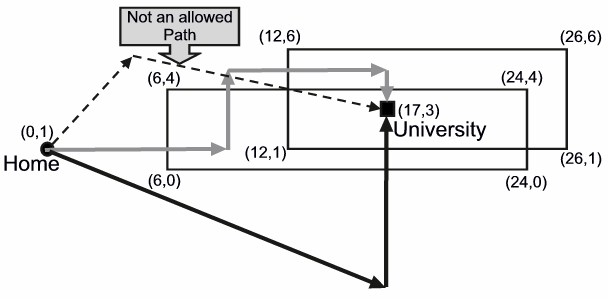
\includegraphics[width=0.7 \textwidth]{2005f.png}
					\caption{} \label{2005f}
				\end{figure}
				
				马路数 $n \le 500$。
			
			\subsubsection{算法讨论}
				将马路延长后,可得到一个 $N \times M$ 的网格,且  $\mathcal{O}(n) = \mathcal{O}(N) = \mathcal{O}(M) $。实现的过程中,不必实际地将其直接延长,而可使用 时间复杂度 $\mathcal{O}(n \log n)$ 的离散化实现。
				
				这样转化成网格后,问题等价于,从一个格子仅通过相邻的格子走到另一个格子,部分相邻格子间无代价,部分相邻格子间代价为 $1$,问最小代价。这可以用传统的 BFS 算法解决,但与传统做法稍有不同的是,必须先访问代价为 0 的点,再访问代价为 $1$ 的点,这样才能保证队列
%				中的点
				代价单调。BFS 后终点格子的权值就是答案。
			\subsubsection{时空复杂度}
				时间复杂度 $\mathcal{O}\left(n^2 \right)$。
					
				空间复杂度 $\mathcal{O}\left(n\right)$。

\newpage
		\subsection{ACM/ICPC World Finals 2005 G Tiling the Plane}
			\subsubsection{题目大意}
				问一个简单\emph{正交}多边形在不旋转不翻转的情况下,是否能密铺平面。
				
				一个多边形能密铺平面当且仅当
				\begin{enumerate}
					\item 边界上存在有序的四点 $A,B,C,D$,使得有向的一段边界 $AB$ 与 有向边界 $DC$ 在平移后重合;或者
					\item 边界上存在有序的六点 $A,B,C,D,E,F$,使得有向的一段边界 $AB$ 与 有向边界 $ED$ 在平移后重合,且有向边界 $BC$  与有向边界 $FE$  平移后重合,还要有向边界 $CD$  与有向边界 $AF$  平移后重合。
				\end{enumerate}
				多边形顶点数 $n \le 50$。边界保证与坐标轴平行。
			\subsubsection{算法讨论}
				为了简化问题,不妨先将方向相同的两段相邻的边合并成一段。此操作不影响答案。
				
				为了高效地使用好题目给出的定理,我们预处理 $F[a][b][l]$ 表示从多边形顶点 $a$ 开始顺数 $l$ 个顶点的有向路径与 $b$ 开始倒数 $l$ 个顶点的有向路径的逆是否在平移后重合。此操作可在 $\mathcal{O}\left(n^4 \right)$ 的时间内实现——枚举 $a, b, l$ 耗时 $\mathcal{O}\left(n^3 \right)$,再模拟 耗时  $\mathcal{O}\left(n \right)$。
				
				不妨以第二条规则来阐述我们最终的判定算法,第一条规则同理。首先,如果答案为是,则要求 有向边界 $AD$ 的长度等于 有向边界 $DA$ 的长度。又多边形的总边数已经确定,换言之,确定了 $A$ 就确定了 $D$。同理, 确定了 $B, C$ 就确定了 $E,F$。这样枚举只需 $\mathcal{O}\left(n^3 \right)$ 时间。对于枚举出来的点的判定,只需求出相邻点间的长度 $l$,使用刚才预处理的 $F[\cdot][\cdot][\cdot]$,看看它们是否都为真。如果是,则立即返回能密铺;否则找不到这样的六元组,返回不能密铺。
				
				这个判定
%				规则
				法则
				的证明涉及到 \emph{希尔伯特第十八问题} 。笔者暂时无法给出该命题的证明。
			\subsubsection{时空复杂度}
				时间复杂度 $\mathcal{O}\left(n^4 \right)$。
					
				空间复杂度 $\mathcal{O}\left(n\right)$。


\newpage
		\subsection{ACM/ICPC World Finals 2005 H The Great Wall Game}
			\subsubsection{题目大意}

%				网格
				如图 \ref{2005h},大小 $n \times n$ 的网格中有若干棋子。每个棋子一次可往四个方向移动一步,且一个格子中不能同时存在两个棋子。问将其摆成以一横行,一纵列,或者一个对角线需至少移动几步?
				
				\begin{figure}[htb]
					\centering
					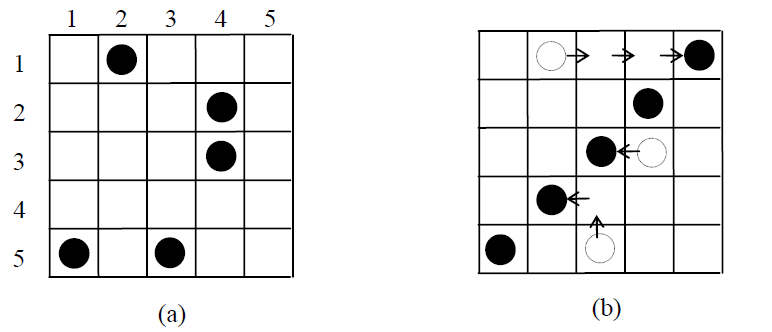
\includegraphics[width=0.7 \textwidth]{2005h.png}
					\caption{} \label{2005h}
				\end{figure}
				
				$n \le 15$。
			\subsubsection{算法讨论}
				分析可知 一个格子中是否可以同时存在两个棋子不影响答案,因为棋子之间没有分别,如果两个棋子互相穿越了对方,那么相当于在穿越对方的一瞬间角色互换,这样就不存在穿越事件了,而且这种情况下的答案可能会更小。不妨忽略此条件。
				
				问题即,给每个棋子分别指定一个终点,两两之间走最短路,代价为最短路之和。问什么样的指定方案最优?这样就是一个带权二分匹配的问题。枚举究竟是要在哪一行,哪一列,或者对角线设定终点,并抽象为左支的 $n$ 个点;再设 $n$ 个棋子为右枝的 $n$ 个点,左右支之间的点连边,代价为其间的最短路长度。答案即最小匹配的代价。
			\subsubsection{时空复杂度}
				时间复杂度 $\mathcal{O}\left(F(n) \right)$。 $F(n)$ 表示求解 $n$ 个点的带权完全二分图的最优匹配的时间,因具体使用的算法而异。
					
				空间复杂度 $\mathcal{O}\left(n^2\right)$。
				

\newpage
		\subsection{ACM/ICPC World Finals 2005 I Workshops}
			\subsubsection{题目大意}
				有 $N$ 个队伍,每个队伍有 $a_i$ 个人,需要开一个 $b_i$ 分钟的会议。同时有 $M$ 个房间,每个房间能容纳不超过 $A_i$ 个人,并只开放 $B_i$ 分钟,且最多被一个队伍使用。一个队伍最多使用一个房间。问最少有多少队伍不能参加会议;并在此基础上,最少有多少人不能参加会议。
				
				$N, M \le 1000$。
			
			\subsubsection{算法讨论}
				我们给出一个贪心算法 \ref{2005i}。
				\begin{algorithm}[H]
				\caption{}
				\label{2005i}
					\begin{algorithmic}[1]
						\For{按照 $B_i$ 从小到大的顺序枚举 $(A_i, B_i)$} 
								\State $S \gets \left\{a_j| a_j \le A_i, b_j  \le B_i, j \text{ 未曾被选择}\right\}$
								
								\If{
%									有这样的 $p$
								$S \ne \varnothing$
								}
									\State $p \gets S$ 中 $a_j$ 最大的 $j$。
									\State 将 $(a_p, b_p)$ 与  $(A_i, B_i)$ 配对,并标记 $p$ 被选择。
								\EndIf
%								答案为
						\EndFor
						\State 输出\emph{未被选择}的 $p$ 的数量及其 $a_p$ 之和。
					\end{algorithmic}
				\end{algorithm}	
				\begin{theorem}
					贪心算法 \ref{2005i} 能导出正确答案。
				\end{theorem}
				\begin{pf}
					我们假设某一个枚举的房间  $(A_i, B_i)$ 没有与最优的队伍 $(a_p, b_p)$ 配对,而与另一队伍  $(a_q, b_q)$  配对了。接下来分两种情况 
					\begin{enumerate}
						\item 如果    $(a_p, b_p)$   未与其他房间配对。注意到匹配的关系不会更改,那么使用调整法,直接将 $(A_i, B_i)$ 的对象更改为  $(a_p, b_p)$,不能参加会议的队伍数没变,不能参加会议的人不会变多,答案不会变差。
						\item 如果    $(a_p, b_p)$ 与 $(A_j, B_j)$  配对了。注意到 $(A_i, B_i)$  能匹配不优的   $(a_q, b_q)$,故
							$a_q \le a_p % \le A_i
						, b_q \le B_i$。又由于当时  $(a_p, b_p)$  未与其他房间匹配,可供   $(A_i, B_i)$ 选择,故一定有 $B_i \le B_j$。 $(A_j, B_j)$   配    $(a_p, b_p)$,故 $a_p \le A_j $ 合起来得到
							\begin{align}
								a_q \le a_p \le A_j \\
								 b_q \le B_i \le  B_j
							\end{align}
							故 $(a_q, b_q)$ 也能和 $(A_j, B_j)$ 配对。这样使用调整法直接交换这两对就可以得到新解,且答案不变化。
					\end{enumerate} 
					而如果   $(A_i, B_i)$ 没有与任何的队伍配对,那么直接把 最优的队伍 $(a_p, b_p)$  抢过来也能得到一个新解,答案不会变差。
					故总可以调整为  $(A_i, B_i)$ 与最优的队伍 $(a_p, b_p)$ 配对的较优解。
					
					重复上述过程,最终肯定可得到贪心解,而答案较初始解不会变差,又由初始解有任意性,综上,贪心算法 \ref{2005i} 能导出正确答案。\qed
				\end{pf}
					直接运行 贪心算法 \ref{2005i} 即可。
					\subsubsection{时空复杂度}
						时间复杂度 $\mathcal{O}\left(NM \right)$。
					
						空间复杂度 $\mathcal{O}\left(N + M\right)$。


\newpage
		\subsection{ACM/ICPC World Finals 2005 J Zones}
			\subsubsection{题目大意}

				如图 \ref{2005j},有
%				若干
				$N$ 个
				待建的基站,每个基站覆盖的范围是一个等圆。每个基站能服务的人数给定,同时有些基站之间有交集,也在输入中给出。选择开通哪 $M$ 个基站,能使得被服务的人数最多,并求出此人数。基站间的交集共有 $K$ 处。
				
				\begin{figure}[htb]
					\centering
					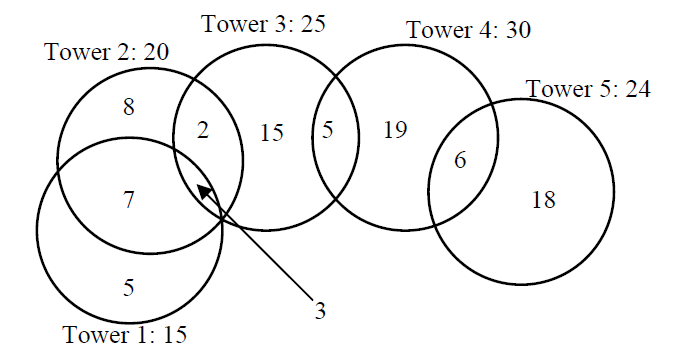
\includegraphics[width=0.6 \textwidth]{2005j.png}
					\caption{} \label{2005j}
				\end{figure}
				
				$M \le N \le 20,
					%, M \le 10
				 K \le 10$。
			\subsubsection{算法讨论}
				为了处理方便,先把有交集的部分从各个基站的人数中扣除。
				
				不妨直接枚举选择了哪 $M$ 个点,再枚举这 $K$ 个有交集的地方,看看其中是否有一个点(或更多)被选择。若是,则将交集的人数加回答案,取最优值返回。
				
				可将选择的点和每处交集涉及的基站用位
				% 运算
				表示出,加快速度。	
			\subsubsection{时空复杂度}
				时间复杂度 $\mathcal{O}\left(\binom{N}{M} \cdot N K \right)$。配合位运算,速度超快。
					
				空间复杂度 $\mathcal{O}\left(KN\right)$。
\newpage
	
	\section{ACM/ICPC World Finals 2004}
		\subsection{ACM/ICPC World Finals 2004 A Carl the Ant}
			\subsubsection{题目大意}
				有若干只蚂蚁从地下穿到地面,行走一段距离后,穿回洞穴。
				
				蚂蚁以相同时间间隔 $d$ 出洞。
				
				有一只蚂蚁在最前面带路,且在路上的行走过程中都沿着每格为单位长度的网格格线走(起点和终点位于网格格点)。其他蚂蚁则跟着带队的蚂蚁留下的气味走。
				
				每支蚂蚁长度均为单位长度,速度均为单位速度,且会沿着带队的蚂蚁\emph{最新}留下的气味走。
				
				如果两只蚂蚁接下来会碰撞,那么\emph{等待了最久的蚂蚁先走},而如果两只蚂蚁等待的时间相同,那么\emph{走了最远路径的先走},另一只蚂蚁则停下。若有蚂蚁在洞口附近停下并堵住洞口,那么洞口的蚂蚁也会排好队,等会依次通过。
				
				问全部蚂蚁回到洞穴的时间及其先后顺序。
				
				带头蚂蚁在路上行走的长度 $N\le 50$,蚂蚁总数 $M \le 100$。$1 \le d \le 100$。
			\subsubsection{算法讨论}
				由于所有的蚂蚁都在网格线上运动,那么使用一个二维数组模拟它们的运动就可以了。二维数组的尺寸 $(2N + 1) \times (2N + 1)$。
				
				需要细心地处理两只蚂蚁将要碰撞时,谁走先谁走后的问题。
%				为了模拟的方便,可在之前对蚂蚁的优先级拍个序,模拟时按照顺序运动。
				模拟时可能需要用到类似 Bellman-Ford 的算法,因为不便于确定移动各个蚂蚁的先后顺序。
				
				按照模拟的结果输出答案。
			\subsubsection{时空复杂度}
				时间复杂度 $\mathcal{O}\left(N^2 + N \cdot \min(M,d)\cdot M k\right)$。 $k$ 是 Bellman-Ford 算法迭代的次数,实践起来此值较小。
					
				空间复杂度 $\mathcal{O}\left(N^2\right)$。


		\newpage
		\subsection{ACM/ICPC World Finals 2004 B Heliport}
			\subsubsection{题目大意}
				如图 \ref{2004b} 中的两例,给出一个正交的简单多边形,求最大的内接圆半径。
				
									\begin{figure}[htb]
\centering
\begin{minipage}{.6\textwidth}
  \centering

\definecolor{ffccww}{rgb}{1,0.8,0.4}
\definecolor{cczzqq}{rgb}{0.8,0.6,0}
\definecolor{cqcqcq}{rgb}{0.75,0.75,0.75}
\begin{tikzpicture}[line cap=round,line join=round,>=stealth',x=1.0cm,y=1.0cm,scale = 0.8]
\draw [color=cqcqcq,dash pattern=on 2pt off 2pt, xstep=1.0cm,ystep=1.0cm] (0,0) grid (7.5,5.5);
\draw[->,color=black] (-0.4,0) -- (7.92,0) node[right] {$x$};
\foreach \x in {,1,2,3,4,5,6,7}
\draw[shift={(\x,0)},color=black] (0pt,2pt) -- (0pt,-2pt) node[below] {\footnotesize $\x$};
\draw[->,color=black] (0,-0.42) -- (0,5.82) node[left] {$y$};
\foreach \y in {,1,2,3,4,5}
\draw[shift={(0,\y)},color=black] (2pt,0pt) -- (-2pt,0pt) node[left] {\footnotesize $\y$};
\draw[color=black] (0pt,-10pt) node[left] {\footnotesize $0$};
\clip(-0.47,-0.42) rectangle (7.92,5.82);
\fill[color=ffccww,fill=ffccww,fill opacity=0.2] (1,5) -- (6,5) -- (6,4) -- (5,4) -- (5,2) -- (7,2) -- (7,1) -- (4,1) -- (4,2) -- (3,2) -- (3,1) -- (1,1) -- (1,2) -- (2,2) -- (2,3) -- (1,3) -- cycle;
\draw [color=ffccww] (1,5)-- (6,5);
\draw [color=ffccww] (6,5)-- (6,4);
\draw [color=ffccww] (6,4)-- (5,4);
\draw [color=ffccww] (5,4)-- (5,2);
\draw [color=ffccww] (5,2)-- (7,2);
\draw [color=ffccww] (7,2)-- (7,1);
\draw [color=ffccww] (7,1)-- (4,1);
\draw [color=ffccww] (4,1)-- (4,2);
\draw [color=ffccww] (4,2)-- (3,2);
\draw [color=ffccww] (3,2)-- (3,1);
\draw [color=ffccww] (3,1)-- (1,1);
\draw [color=ffccww] (1,1)-- (1,2);
\draw [color=ffccww] (1,2)-- (2,2);
\draw [color=ffccww] (2,2)-- (2,3);
\draw [color=ffccww] (2,3)-- (1,3);
\draw [color=ffccww] (1,3)-- (1,5);
\draw(3.5,3.5) circle (1.5cm);
\begin{scriptsize}
\fill [color=cczzqq] (1,5) circle (1.5pt);
\draw[color=cczzqq] (1.1,5.22) node {$A$};
\fill [color=cczzqq] (6,5) circle (1.5pt);
\draw[color=cczzqq] (6.12,5.22) node {$B$};
\fill [color=cczzqq] (6,4) circle (1.5pt);
\draw[color=cczzqq] (6.12,4.24) node {$C$};
\fill [color=cczzqq] (5,4) circle (1.5pt);
\draw[color=cczzqq] (5.12,4.24) node {$D$};
\fill [color=cczzqq] (5,2) circle (1.5pt);
\draw[color=cczzqq] (5.12,2.23) node {$E$};
\fill [color=cczzqq] (7,2) circle (1.5pt);
\draw[color=cczzqq] (7.11,2.23) node {$F$};
\fill [color=cczzqq] (7,1) circle (1.5pt);
\draw[color=cczzqq] (7.12,1.22) node {$G$};
\fill [color=cczzqq] (4,1) circle (1.5pt);
\draw[color=cczzqq] (4.13,1.22) node {$H$};
\fill [color=cczzqq] (4,2) circle (1.5pt);
\draw[color=cczzqq] (4.08,2.23) node {$I$};
\fill [color=cczzqq] (3,2) circle (1.5pt);
\draw[color=cczzqq] (3.11,2.23) node {$J$};
\fill [color=cczzqq] (3,1) circle (1.5pt);
\draw[color=cczzqq] (3.12,1.22) node {$K$};
\fill [color=cczzqq] (1,1) circle (1.5pt);
\draw[color=cczzqq] (1.1,1.22) node {$L$};
\fill [color=cczzqq] (1,2) circle (1.5pt);
\draw[color=cczzqq] (1.12,2.23) node {$M$};
\fill [color=cczzqq] (2,2) circle (1.5pt);
\draw[color=cczzqq] (2.12,2.23) node {$N$};
\fill [color=cczzqq] (2,3) circle (1.5pt);
\draw[color=cczzqq] (2.12,3.23) node {$O$};
\fill [color=cczzqq] (1,3) circle (1.5pt);
\draw[color=cczzqq] (1.12,3.23) node {$P$};
\end{scriptsize}
\end{tikzpicture}
\end{minipage}%
\begin{minipage}{.4\textwidth}
  \centering
\definecolor{ffccww}{rgb}{1,0.8,0.4}
\definecolor{cczzqq}{rgb}{0.8,0.6,0}
\definecolor{cqcqcq}{rgb}{0.75,0.75,0.75}
\begin{tikzpicture}[line cap=round,line join=round,>=stealth',x=1.0cm,y=1.0cm,scale = 0.8]
\draw [color=cqcqcq,dash pattern=on 2pt off 2pt, xstep=1.0cm,ystep=1.0cm] (-0,0) grid (5.2,5.5);
\draw[->,color=black] (-0.4,0) -- (5.68,0) node[right] {$x$};
\foreach \x in {,1,2,3,4,5}
\draw[shift={(\x,0)},color=black] (0pt,2pt) -- (0pt,-2pt) node[below] {\footnotesize $\x$};
\draw[->,color=black] (0,-0.42) -- (0,5.82) node[left] {$y$};
\foreach \y in {,1,2,3,4,5}
\draw[shift={(0,\y)},color=black] (2pt,0pt) -- (-2pt,0pt) node[left] {\footnotesize $\y$};
\draw[color=black] (0pt,-10pt) node[left] {\footnotesize $0$};
\clip(-0.4,-0.43) rectangle (5.68,5.61);
\fill[color=ffccww,fill=ffccww,fill opacity=0.2] (1,5) -- (5,5) -- (5,2) -- (4,2) -- (4,1) -- (1,1) -- cycle;
\draw [color=ffccww] (1,5)-- (5,5);
\draw [color=ffccww] (5,5)-- (5,2);
\draw [color=ffccww] (5,2)-- (4,2);
\draw [color=ffccww] (4,2)-- (4,1);
\draw [color=ffccww] (4,1)-- (1,1);
\draw [color=ffccww] (1,1)-- (1,5);
\draw(2.76,3.24) circle (1.76cm);
\begin{scriptsize}
\fill [color=cczzqq] (1,5) circle (1.5pt);
\draw[color=cczzqq] (1.1,5.21) node {$A$};
\fill [color=cczzqq] (5,5) circle (1.5pt);
\draw[color=cczzqq] (5.12,5.21) node {$B$};
\fill [color=cczzqq] (5,2) circle (1.5pt);
\draw[color=cczzqq] (5.12,2.22) node {$C$};
\fill [color=cczzqq] (4,2) circle (1.5pt);
\draw[color=cczzqq] (4.12,2.22) node {$D$};
\fill [color=cczzqq] (4,1) circle (1.5pt);
\draw[color=cczzqq] (4.12,1.22) node {$E$};
\fill [color=cczzqq] (1,1) circle (1.5pt);
\draw[color=cczzqq] (1.1,1.22) node {$F$};
\end{scriptsize}
\end{tikzpicture}




\end{minipage}
  \caption{}
  \label{2004b}
\end{figure}
				
				多边形点数 $N \le 20$,保证边与坐标轴平行或垂直。
			\subsubsection{算法讨论}
				我们可以给出一个求任意简单多边形(不要求边正交,即与坐标轴平行或垂直)的最大内接圆半径的算法。算法的核心在于说明,肯定存在一个最优的内接圆,与多边形边界交于至少三点。


									\begin{figure}[b]
\centering
\begin{minipage}{.3\textwidth}
  \centering

\definecolor{qqwuqq}{rgb}{0,0.39,0}
\definecolor{qqqqff}{rgb}{0,0,1}
\begin{tikzpicture}[line cap=round,line join=round,>=triangle 45,x=1.0cm,y=1.0cm]
\clip(-0.55,0.24) rectangle (4.95,5.17);
\draw [shift={(3,3)},color=qqwuqq,fill=qqwuqq,fill opacity=0.1] (0,0) -- (90:0.36) arc (90:270:0.36) -- cycle;
\draw [dash pattern=on 3pt off 3pt] (3,0.24) -- (3,5.17);
\draw [domain=-0.5507425556704313:3.0] plot(\x,{(-18--5*\x)/-1});
\draw [domain=-0.5507425556704313:3.0] plot(\x,{(-12--2*\x)/-2});
\draw [domain=-0.5507425556704313:3.0] plot(\x,{(-6-0*\x)/-2});
\draw [domain=-0.5507425556704313:3.0] plot(\x,{(-0-2*\x)/-2});
\draw [domain=-0.5507425556704313:3.0] plot(\x,{(--6-3*\x)/-1});
% \draw [dash pattern=on 3pt off 3pt] (3,-3) -- (3,0.24);
\begin{scriptsize}
\fill [color=qqqqff] (3,3) circle (1.5pt);
\fill [color=qqqqff] (0,3) circle (1.5pt);
\draw[color=qqwuqq] (3.58,3.05) node {$\alpha = \pi$};
\end{scriptsize}
\end{tikzpicture}

  \caption{}
  \label{2004b2}


\end{minipage}%
\begin{minipage}{.4\textwidth}
  \centering
\definecolor{cczzqq}{rgb}{0.8,0.6,0}
\definecolor{ffccww}{rgb}{1,0.8,0.4}
\definecolor{ttffqq}{rgb}{0.2,1,0}
\definecolor{ttzzqq}{rgb}{0.2,0.6,0}
\begin{tikzpicture}[line cap=round,line join=round,>=triangle 45,x=1.0cm,y=1.0cm, scale = 0.65]
\clip(-3.45,-2.26) rectangle (5.36,5.36);
\fill[color=ttffqq,fill=ttffqq,fill opacity=0.1] (-1,3) -- (0,5) -- (2,5) -- (3,3) -- (5,2) -- (4,-2) -- (-2,-2) -- (-3,2) -- cycle;
\draw [color=ttffqq] (-1,3)-- (0,5);
\draw [color=ttffqq] (0,5)-- (2,5);
\draw [color=ttffqq] (2,5)-- (3,3);
\draw [color=ttffqq] (3,3)-- (5,2);
\draw [color=ttffqq] (5,2)-- (4,-2);
\draw [color=ttffqq] (4,-2)-- (-2,-2);
\draw [color=ttffqq] (-2,-2)-- (-3,2);
\draw [color=ttffqq] (-3,2)-- (-1,3);
\draw [line width=2pt,color=ffccww] (1,1.51) circle (2.49cm);
\draw [line width=2pt,color=cczzqq] (1,1.1) circle (2.76cm);
\begin{scriptsize}
\fill [color=ttzzqq] (-1,3) circle (1.5pt);
\draw[color=ttzzqq] (-0.8,3.43 - 1) node {};
\fill [color=ttzzqq] (3,3) circle (1.5pt);
\draw[color=ttzzqq] (3.23,3.43) node {};
\fill [color=ttzzqq] (1,1.51 - 1) circle (1.5pt);
\draw[color=ttzzqq] (1.21,1.94 - 0.8) node {$P$};
\fill [color=ttzzqq] (1,1.1) circle (1.5pt);
\draw[color=ttzzqq] (1.24,1.53 - 1) node {$P^\prime$};
\end{scriptsize}
\end{tikzpicture}

  \caption{}
  \label{2004b3}
\end{minipage}%
\begin{minipage}{.3\textwidth}
  \centering
\definecolor{qqzzcc}{rgb}{0,0.6,0.8}
\definecolor{ffzzzz}{rgb}{1,0.6,0.6}
\definecolor{zzttqq}{rgb}{0.6,0.2,0}
\begin{tikzpicture}[line cap=round,line join=round,>=triangle 45,x=1.0cm,y=1.0cm]
\clip(-2.42,2.56) rectangle (1.28,4.38);
\fill[color=zzttqq,fill=zzttqq,fill opacity=0.1] (-2,4) -- (1,4) -- (1,3) -- (-2,3) -- cycle;
\draw [color=zzttqq] (-2,4)-- (1,4);
\draw [color=zzttqq] (1,4)-- (1,3);
\draw [color=zzttqq] (1,3)-- (-2,3);
\draw [color=zzttqq] (-2,3)-- (-2,4);
\draw [line width=1.5pt,color=qqzzcc] (-1.5,3.5) circle (0.5cm);
\draw [line width=1.5pt,color=qqzzcc!70!white] (0,3.5) circle (0.5cm);
\begin{scriptsize}
\fill [color=ffzzzz] (-1.5,3.5) circle (1.5pt);
\draw[color=ffzzzz] (-1.35-0.15,3.78) node {$P^\prime$};
\fill [color=ffzzzz] (0,3.5) circle (1.5pt);
\draw[color=ffzzzz] (0.16-0.15,3.78) node {$P$};
\end{scriptsize}
\end{tikzpicture}
  \caption{}
  \label{2004b4}
\end{minipage}
\end{figure}


				{\theorem 存在一个最优的内接圆,与多边形边界交于至少三点。}
				\begin{pf}


					不妨假设其只交于两点,作出圆心,那么肯定存在一个方向,使得圆心向该方向运动后,不会更靠近两个点。因为如图 \ref{2004b2},如果圆心要靠近一个点,那么需要向长度为 $\pi$ 的一个开区间中的一个方向运动。两个这样的区间必然无法覆盖区间 $[0, 2\pi)$,随便选一个未被覆盖的角度,就是我们要找的方向。
					
					随后,只要将圆心向这个方向运动无穷小量,并在固定圆心之后,将半径取最大的可能值,就可以得到一个新解,且答案不会变差。例如图 
  \ref{2004b3},将圆心 $P$ 移动到 $P^\prime$。
					
					若继续移动,那么此圆总会碰到边界,与边界交于第三个点,例如 图 \ref{2004b4},将圆心 $P$ 移动到 $P^\prime$。而这样做答案不会更差
%					,
					。又初始解具有任意性,故根据调整法,此情况下命题得证。
					
					而若只有一个交点,或没有交点,
					证明
					同理
%					可证
					。\qed

				\end{pf}
				
				那么只要在多边形边界上枚举三点,求出一个最好的圆心就可以了。但是,多边形边界上的点有无穷多个。我们应分以下情况枚举交点(或交点
%				位于
				所在的边界),计算可能的最优圆心:
				\begin{enumerate}
					\item {\bf 三个交点均为多边形顶点}:直接求对应三角形的外心,具体地,求中垂线之交。
					\item{\bf  只有两个交点为多边形顶点}:此时圆过两定点,并与一条直线(第三点所在的边)相切。此时可求出两个顶点的中垂线,并以参数方程的形式,表示成点 $(a+b t, p + qt)$。求出其到此直线的距离 $d$。$d$ 应该与 $(a+b t, p + qt)$ 到两个顶点中任意一个的距离相同,以此建立方程,解参数 $t$,代回  $(a+b t, p + qt)$ 即为圆心。
					\item {\bf 只有一个交点为多边形顶点}:此时圆过一定点,并与两条直线相切。如果两线相交,此时可先作出两直线的角平分线(有两条,需分别考虑。),并同样地以参数方程 $(a+b t, p + qt)$ 表示。$(a+b t, p + qt)$  到 两线的距离与到 定点的距离应该相同,建立方程可解出  $t$,代回  $(a+b t, p + qt)$ 即为圆心。而若两线平行,那么作出到它们等距,且与它们平行的线,用同样的方法建立并解出方程,可求出圆心。
					\item {\bf 没有一个交点为多边形顶点}:那么需作出与三条直线均相切的圆,即求三角形内心。具体地,求出角平分线之交即可导出圆心。
				\end{enumerate}
				
				求到可能的圆心后,求出其到边界的最短距离。可以枚举多边形的边界,求点和\emph{线段}的距离,取最小值。此值就是该圆心对应的最大半径。
%				再
				求出所有圆心中,最大半径值最大的。这个值就是答案。
			\subsubsection{时空复杂度}
				时间复杂度 $\mathcal{O}\left(N^4\right)$。枚举点点点/点点边/点边边/边边边 $\mathcal{O}\left(N^3\right)$,再求圆心 $\mathcal{O}\left(1\right)$,再求最大半径 $\mathcal{O}\left(N\right)$。
					
				空间复杂度 $\mathcal{O}\left(N\right)$。\newpage
		\subsection{ACM/ICPC World Finals 2004 C Image Is Everything}
			\subsubsection{题目大意}
				一个 $N \times N \times N$ 的立体网格图形,每个格子里可能是一个有颜色的不透明立方块,或者什么都没有(透明)。
				
				给出它六个方向上的视图,问\emph{最多}有多少个格子里有立方块?
				
				保证有解。 $N \le 10$。
			\subsubsection{算法讨论}
				由于要最大化有立方块的格子,那么对于每个方向的视图,如果某一格有颜色,就要使得这一格上实际看到的立方快深度越浅越好(离观察者越近越好)。
				
				类似于 Bellman-Ford 的算法 \ref{2004c} 可以实现上述目标。
				\begin{algorithm}[H]
				\caption{}
				\label{2004c}
					\begin{algorithmic}[1]
						\State 图形 $F[\cdot][\cdot][\cdot] \gets \text{ 未知 }, OK \gets $ 真
						\For{$OK$}
							\State $OK \gets $ 假
							\For{枚举所有方向,以及该方向上视图的格子,记其颜色为 $c$}
								\For{深度 $d$。从 $d = 1$ 枚举到 $d = N$}
									\State 计算出该方向,该网格,该深度对应的三维坐标 $(x, y, z)$。
									\If{$c = \text{透明}$且 $F[x][y][z] \ne$ 透明}
										\State $F[x][y][z] \gets\text{透明} , OK \gets $ 真 \Comment{该格透明板上钉钉。}
									\EndIf
									\If{$c \ne\text{透明} $且 $(F[x][y][z] = \text{未知} \lor F[x][y][z] =  c)$ }
										\State $F[x][y][z] \gets c$,并跳出枚举 $d$ 的循环。
									\EndIf
%									\If{$c \ne\text{透明} $且 $F[x][y][z] = c$}
%										\State 跳出枚举 $d$ 的循环。
%									\EndIf
									\If{$c \ne \text{透明} $且 $F[x][y][z] \ne c$}
										\State $F[x][y][z] \gets\text{透明} , OK \gets $ 真 \Comment{产生矛盾
%										,只能改回透明
										}
									\EndIf
								\EndFor
							\EndFor
						\State 输出满足 $F[x][y][z] \ne \text{透明} $   的三元组数。 \Comment{$F[x][y][z]  = \text{未知}$ 的是无法被观察到的
%						格子
						}
						\EndFor
					\end{algorithmic}
				\end{algorithm}	
			\subsubsection{时空复杂度}
				时间复杂度 $\mathcal{O}\left(k N^3\right)$。 $k$ 是  Bellman-Ford  迭代的次数。 $N \le 10$,算法肯定运行得很快。
					
				空间复杂度 $\mathcal{O}\left(N^3\right)$。
		\newpage
		\subsection{ACM/ICPC World Finals 2004 D Insecure in Prague}
			\subsubsection{题目大意}
				有一种加密算法,加密一个只有大小写拉丁字母的字符串 $S$。
				
				记 $N = |S|$。具体地,其工作原理为,取 $M \ge 2 N, 0 \le s, t, i, j < m, \emph{i < j}$,其中 $M$ 是加密串的长度,那么先将加密串的各个位置清空,然后从第 $s$ 个位置起,每隔 $i$ 个空格放一个字母地,将 $S$ 填入到加密串中。紧接着,再从第 $t$ 个空位起,每隔 $j$ 个空格放一个字母地,将 $S$ 再次填入到加密串中。如果达到了加密串末尾,那么跳到开头继续数空格。最后,将剩下的空位随机地乱填入一些字母,加密就完成了。
				
				给出一个加密串,求可能的原串。如果有多解,则不必输出答案,输出相关提示信息即可。
				
				$M \le 40$。
			\subsubsection{算法讨论}
				枚举 $s, t, i, j$,模拟此加密算法,检查两次填入的单词是否相同即可。
				
				对于一个长度固定的空串,如果起始位置和间隔固定,那么接下来填入字母的顺序就固定了,这一步中按顺序访问的位置可以通过预处理求出并记录。模拟加密算法时,可以使用该预处理的信息,直接就可以找到位置,而不必将时间浪费在数空位上。
				
				如果第一步扫描出答案后,剩下的字母中没有第一次曾填入过的字母了,或者数量不足,那么无解,可以直接返回,加快搜索速度。
				
				如果搜到两个解,那么可输出多解信息,退出程序。
			
			\subsubsection{时空复杂度}
				时间复杂度 $\mathcal{O}\left(k + M^5\right)$。$k$ 是预处理的时间,由于 $M \le 40$,所以其非常快。加上前文的减枝,程序运行的速度可以通过数据的检测。
					
				空间复杂度 $\mathcal{O}\left(M^3\right)$。预处理时初始位置不必枚举和记录,只需用偏移处理即可。
		\newpage
		\subsection{ACM/ICPC World Finals 2004 E Intersecting Dates}
			\subsubsection{题目大意}
				有两组日期区间。日期区间就是时间轴上某一天到另一天之间的所有时刻。设两组日期区间的并分别为 $A, B$,求 $B \setminus A$,并用尽量少的日期区间的并来表达 $B \setminus A$。
				
				给出的日期区间中,每一个区间中时刻的年份 $y$ 满足 $\num{1700} \le y \le \num{2100}$。每组日期区间的区间数 $ N, M\le 100$。
			\subsubsection{算法讨论}
				年份介于 $1700$ 和 $2100$ 的日子共有 \num{146462} 天。把日期转化成 $[1,\num{146462}]$ 的整数后,更便于我们的处理。
				
				先考虑求各区间组的并集。我们可以使用扫描线法,将每个区间的左端视为插入事件,右端视为删除事件。时间线扫过去,统计有多少区间插入了之后,仍未删除,即为包含了该时间线所在时刻的区间数。如果该值 $> 0$,那么这个时刻就在并中。
				
				由于涉及到的天数非常有限,所以不必对区间排序离散化,直接在一个长度为 \num{146462} 的离散线性表中操作即可。在对应位置上记录差分(插入事件 $= +1$,删除事件 $= -1$),扫一遍求出和分,$ > 0$ 的元素就在并中;反之,其不在并中。
				
				求出 $A, B$ 后,考虑到  $B \setminus A$ 就是在 $B$ 中的和分 $> 0 $ 但在 $A$ 中的和分 $ = 0$ 的元素之集。仍然可以通过扫描法求得。
				
				最后,在 $B \setminus A$ 中将连续的日子作为区间输出即可。
			\subsubsection{时空复杂度}
				时间复杂度 $\mathcal{O}\left(N + M\right)$。\num{146462} 已被视为常数。
					
				空间复杂度 $\mathcal{O}\left(1\right)$。
		\newpage
		\subsection{ACM/ICPC World Finals 2004 G Navigation}
			\subsubsection{题目大意}
				平面上有
%				若干
				$N$ 个卫星,还有一辆汽车。卫星的起始坐标,运动方向和速度已知。$t = t_0$ 时刻,汽车收到了每个卫星于时刻 $t = t_i < t_0$ 发射的信号。无线信号的波速已知。给定终点,问汽车驶向终点的
%				方位角
				 方向(角度)。

				如果仅通过信号,能计算出两个以上的汽车可能位置,或者信号有误,无法计算出汽车的位置,需分别输出各自的提示信息。容忍 $\num{0.1}$ 的误差,即距离相差 0.1 的两点认为相同。
				
				$N \le 10$。
			\subsubsection{算法讨论}
				由于各个卫星发射信号的时间  $t = t_i$,运行速度和方向,起始坐标都已知,那么可以计算出发射信号时卫星的位置,以及信号从发射到接收的时间间隔。乘上已知的信号波速,即为发射信号时,卫星到汽车的距离。几何化地,以发射信号时的卫星位置为圆心,以及此时卫星到汽车的距离
%				的
				为
				半径作圆,那么汽车就位于此圆上。
				
				$N$ 个卫星就有 $N$ 个圆,将这些圆交起来,就是汽车可能的位置。如果此交集合有超过两个元素或者没有元素,那么应输出相关信息,否则汽车的位置就是这个唯一的元素,使用反正切等反三角函数就可以求到汽车向终点的方向。下讨论如何求交集。
				
				不妨去除重合的圆。如果圆退化成点,即半径为 $0$,那么交集最多就只有这一个圆心。检查下其他圆是否过它,从而就可以确定汽车的位置。如果只有一个圆,且半径为正,那么交集合的势为一级无穷大 $\aleph_1$,汽车的位置不确定。
				
				经过以上处理后,至少存在两个圆,任意圆半径 $> 0$,且任意两圆不重合。不妨随便取两个圆,相交后可能有 $0, 1, 2$ 个交点。将这些点代入到所有圆中检查一遍,就可以知道那些在交集里了。需要小心处理题中的 $ 0.1$ 的误差。
				
				求两圆之交的方法是,将其中一圆表示为参数形式 $\mathbf{p} = (x + r \cos \theta, y + r \sin \theta)$ 代入另一圆的方程 $(\mathbf{p} - \mathbf{q})^2 = r_2^2$,解 $\theta$。具体地,设另一圆圆心 $\mathbf{q} = (x_2, y_2)$	那么就有
				\begin{align}
					(x - x_2 + r \cos\theta)^2 + (y - y_2 + r \sin\theta)^2 & =  r_2^2 \\
					\intertext{展开化简}
					r^2 + (x - x_2)^2 +2 \cdot (x - x_2) \cdot r \cos\theta 
					+ (y - y_2)^2 + 2 \cdot (y - y_2)\cdot r \sin\theta & =  r_2^2 \\
					\intertext{令 $R = \sqrt{(x - x_2)^2 + (y - y_2) ^2}, (\cos \alpha, \sin \alpha) =( (x - x_2)/R, (y - y_2) / R)$}
						 r^2 + (x - x_2)^2 + (y - y_2)^2  + 2 r R \cos(\alpha - \theta) & =  r_2^2  
%					\intertext{最后使用反三角}
%					\theta  =  \alpha  + \cos^{-1} \frac{r_2^2  - r^2 - (x - x_2)^2 -  (y - y_2)^2}{2 r R} + 2k\pi, k \in \mathbb{Z}
				\end{align}最后使用反三角
				\begin{align}
					\theta  =  \alpha  + \cos^{-1} \frac{r_2^2  - r^2 - (x - x_2)^2 -  (y - y_2)^2}{2 r R} + 2k\pi, k \in \mathbb{Z}
				\end{align}
				代回 $(x + r \cos \theta, y + r \sin \theta)$ 就是交点坐标。

			\subsubsection{时空复杂度}
				时间复杂度 $\mathcal{O}\left(N\right)$。
					
				空间复杂度 $\mathcal{O}\left(N\right)$。
		\newpage
		\subsection{ACM/ICPC World Finals 2004 H Tree-Lined Streets}
			\subsubsection{题目大意}
				平面上有 $N$ 条线段,保证每条线段长度为正,
				且
				两两的交点不会是某一个线段的端点。每条线段的长度都不是 $25$ 的整数倍。今要求在这些线段上选若干点,要求
				\begin{enumerate}
					\item 同一线段上相邻的两点间的距离 $\ge k_1 = 50$。
					\item 选择的所有点与任意两线段的交点之间的距离 $\ge k_2 = 25$。
				\end{enumerate}
				问最多能选多少点。
				
				$N \le 100$。
			\subsubsection{算法讨论}
				由于 $k_1 \le 2 k_2$。那么就顺着交点将每条线段分为若干段,这样不同的段之间的选择点的距离必然 $\ge 2k_2 \ge k_1$。所以不妨求出交点将线段分段后分别考虑就可以了,这样不会影响答案。
				
				设某一段的长度为 $l$,如果此段有一个端点,那么 $l$ 增加 25,有二个端点则 $l$直接增长 50。
				那么根据数学知识,这一段上面最多能选
				\begin{align}
					f(l) = \left\lfloor l / 50 \right\rfloor
				\end{align}
				个点。对于每一段 $l$,都计算出对应的 $f(l)$ 后求和,就是答案。
				
			\subsubsection{时空复杂度}
				时间复杂度 $\mathcal{O}\left(N^2\right)$。
					
				空间复杂度 $\mathcal{O}\left(N^2\right)$。
				
		\newpage
		\subsection{ACM/ICPC World Finals 2004 I Suspense!}
			\subsubsection{题目大意}
				例如图 \ref{2004i},有两栋楼,每层楼均高 $\SI{3}{\meter}$,窗户下端离地 $\SI{1}{\meter}$,窗户高度 $\SI{1.5}{\meter}$,窗户上端离天花板$\SI{0.5}{\meter}$。两楼间的距离将会给出。
				
				在某两个给定的窗口下端间拉一根索桥,并且在水平方向上均匀负重,重物是一个平板,通过水平方向上等距离地拉线索实现。可以证明索桥的线缆呈抛物线状,且要求平板离抛物线最低点的高度恰好为 \SI{1}{\meter},且离地至少 \SI{1}{\meter},在拉绳索的两个窗户下端以下至少  \SI{2}{\meter}。
				
				有些楼层有猫,有些楼层有鸟,但同一栋,同一层楼里,两种生物不会同时出现。猫可以往下一次跳\emph{低于} \SI{3}{\meter} 的距离,往上一次跳\emph{低于} \SI{0.5}{\meter} 的距离,鸟不会动。
				
				问索桥的线缆至多能有多长,能使得猫不能仅通过木板接触到鸟?
				
				楼层数 $N \le 25$。
				
				
				\begin{figure}[htb]
					\centering
					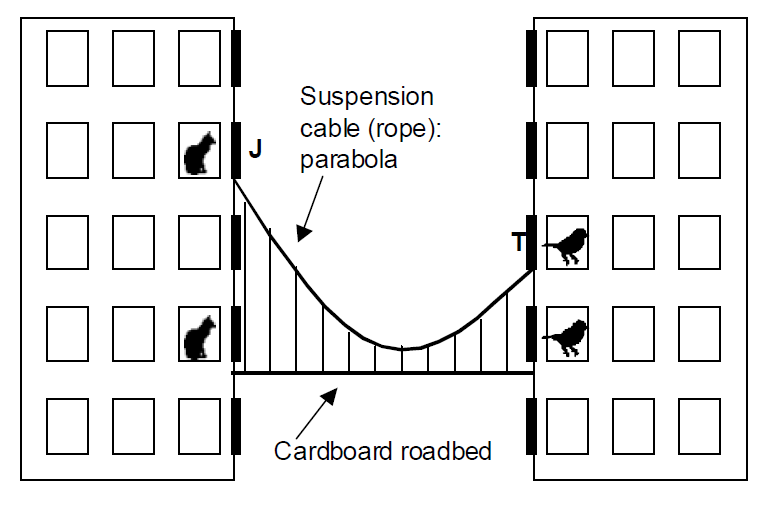
\includegraphics[width=0.7 \textwidth]{2004i.png}
					\caption{} \label{2004i}
				\end{figure}

				\begin{algorithm}[b]
				\caption{}
				\label{2004i}
					\begin{algorithmic}[1]
						\State $Ans  \gets \text{无解}$
						\For{
%							枚举 $i$, 从
							$i = 1$ 到 $ \text{挂绳索的两个楼层中的较低者} - 1$
						}
							\If{两栋房子的第 $i$ 层楼中,一栋有猫,一栋有鸟}
								\State $Ans \gets 3i-2$,并退出循环。 
							\EndIf
							\If{两栋房子的第 $(i + 1)$ 层楼中至少有一栋有猫,第 $i$ 层楼中至少有一栋有鸟}
								\State $Ans \gets 3i-1.5$,并退出循环。 
							\EndIf
						\EndFor
					\end{algorithmic}
				\end{algorithm}	
				
			\subsubsection{算法讨论}
				根据生活经验,绳索越长,平板低,故需要求出平板最低的高度。
%				绳索越长平板越低的结论稍后证明。
				
				通过题目给出的常量,用算法 \ref{2004i} 即可求出此最低高度 $Ans$。
				
				求出高度 $Ans$ 后,就要通过物理手段求绳索的长度了。
				
				{\theorem 线缆呈抛物线形。}
				
				\vskip0.5em

\begin{tabular}{p{.3\textwidth} p{.6\textwidth}}
    \vspace{0pt} 
\centering
\definecolor{cczzqq}{rgb}{0.8,0.6,0}
\definecolor{qqzzff}{rgb}{0,0.6,1}
\begin{tikzpicture}[line cap=round,line join=round,>=stealth',x=1.0cm,y=1.0cm]
\draw[->,color=black] (-0.5,0) -- (3.34,0) node[right] {$x$};
%\foreach \x in {1,2,3}
%\draw[shift={(\x,0)},color=black] (0pt,2pt) -- (0pt,-2pt) node[below] {\footnotesize $\x$};
\draw[->,color=black] (0,-0.5) -- (0,7.75) node[left] {$y$};
%\foreach \y in {-1,1,2,3,4}
%\draw[shift={(0,\y)},color=black] (2pt,0pt) -- (-2pt,0pt) node[left] {\footnotesize $\y$};
\draw[color=black] (0pt,-10pt) node[left] {$O$};
\newcommand{\lenghtlengthiii}{2.5}
\draw [samples=50,rotate around={0:(0,0)},xshift=0cm,yshift=0cm,color=cczzqq,domain=0:\lenghtlengthiii)] plot (\x,{(\x)^2});
\draw [color=qqzzff, -> ] (0,0) -- (-0.8,0) node[above] {$\mathbf{F}$};
\draw [color=qqzzff, -> ] (\lenghtlengthiii,\lenghtlengthiii*\lenghtlengthiii) -- 
		({\lenghtlengthiii + 1.2*sqrt(\lenghtlengthiii*\lenghtlengthiii*4+1)/(\lenghtlengthiii*\lenghtlengthiii*4+1)},
		{\lenghtlengthiii * \lenghtlengthiii + 1.2* 2 * \lenghtlengthiii *sqrt(\lenghtlengthiii*\lenghtlengthiii*4+1)/(\lenghtlengthiii*\lenghtlengthiii*4+1)}) node[above] {$\mathbf{F}_2$};
%\draw[shift={(\lenghtlengthiii,0)},color=black] (0pt,2pt) -- (-0pt,-2pt) 
%		node[below 
%		right
%		] {$x$}
%		;
\fill [color=qqzzff] (0,0) circle (1.5pt);
\fill [color=qqzzff] (\lenghtlengthiii,\lenghtlengthiii*\lenghtlengthiii)  circle (1.5pt)
node[above left,color=black
		] {$P$};

\foreach \x in {1,2,3,4,5}
\draw [color=qqzzff, -> ] (\x * \lenghtlengthiii / 5,\x * \lenghtlengthiii / 5*\x * \lenghtlengthiii / 5 ) -- 
		 (\x * \lenghtlengthiii / 5,0);
\draw [color=qqzzff, below] (\lenghtlengthiii / 2, 0) node {$\mathbf{G} = (0, -\rho x)$};
\end{tikzpicture}
				\captionof{figure}{}
				\label{2004i2}
    & 
    \vspace{0pt}
				\begin{pf}
					如图 \ref{2004i2} 将线缆的最低点平移到原点 $O$。设线缆可表达为函数 $y(x)$。任取另外一点$P(x, y(x))$,分析 $O$ 到 $P$ 的绳索的受力。原点处有一个水平的拉力 $\mathbf{F} = (-F, 0)$,$P(x, y(x))$ 处有一个沿切线方向的力 $\mathbf{F}_2$。
%					绳索处处受力相等,故 $|\mathbf{F}| = |\mathbf{F}_2|$。
					负重的线密度 $\rho$,水平方向的长度 $x$,故总负重 $\mathbf{G} = (0, -\rho x)$。整段绳子动量 $\mathbf{p} \equiv \mathbf{0}$,故
					\begin{align}
						\mathbf{F} + \mathbf{F}_2 + \mathbf{G} = \mathbf{0}
					\end{align}
					即
					\begin{align}
						\begin{cases}
							-F + F_2\cos\theta + 0 = 0\\
							0 +  F_2\sin\theta - \rho x = 0\\
							\tan\theta  = 
%								\left. \mathrm{d} y(x) / \mathrm{d} x \right|_{x}
								\mathrm{d} y(x) / \mathrm{d} x
						\end{cases}
					\end{align}
					整理可得
					\begin{align}
						\frac{\mathrm{d} y(x)}{ \mathrm{d} x} = \tan\theta = \frac{\rho x}{F}
					\end{align}
					分离变量,积分
					\begin{align}
						\int F \mathrm{d} y(x) =  \int \rho x\mathrm{d} x + \mathrm{C}
					\end{align}
					即 
					\begin{align}
						y(x) = \frac{\rho}{2 F} x^2 + \mathrm{C}
					\end{align}
					$\rho / (2 F)$ 为与绳子有关的常数,故命题得证。 
					 \qed
				\end{pf}
\end{tabular}
			令 $\rho / (2 F) = a$。在固定了平板的高度后,也就确定了抛物线的最低点,以及到两个窗户的竖直距离 $h_{1,2}$。接下来需要确定 $a$ 和最低点到两个窗户的水平距离。即求 $a, x_1, x_2$ 满足
			\begin{align}
				ax_1^2 &= h_1 \label{2004iaaa}\\
				ax_2^2 &= h_2 \label{2004ibbb}\\
				x_1 + x_2 &= L \label{2004iccc}
			\end{align}
			其中 $L$ 是
%			两栋
			房屋间的距离。
			$\sqrt{\eqref{2004iaaa}} + \sqrt{\eqref{2004ibbb}}$ 得
			\begin{align}
				\sqrt{a} L& = \sqrt{a}x_1 + \sqrt{a}x_2 = \sqrt{h_1} + \sqrt{h_2}
				\intertext{故}
					a &= \left(\left.\left(\sqrt{h_1} + \sqrt{h_2}\right) \right/ L \right)^2\\
					x_1 &= \sqrt{h_1 / a}\\
					x_2 &= \sqrt{h_2 / a}
			\end{align}
			这样最后的问题就是求曲线 $y = f(x) = ax^2, x \in [-x_1, x_2]$ 的长度 $l$。根据微积分知识,答案应当为
			\begin{align}
				l & =\int_{-x_1}^{x_2} \sqrt{{\mathrm{d} x}^2 + {\mathrm{d} y}^2} \notag \\
					& =\int_{-x_1}^{x_2} \mathrm{d} x \sqrt{1 + {(\mathrm{d} y /\mathrm{d} x)}^2} \notag  \\ 
					& =\int_{-x_1}^{x_2} \sqrt{1 + {(2ax)}^2} \mathrm{d} x \notag  \\ 
					& = \left[ \frac{2 a x \sqrt{4 a^2 x^2+1} + \sinh^{-1}2 a x}{4 a}\right]_{-x_1}^{x_2} \label{2004id}
			\end{align}
			根据 \eqref{2004id} 就可直接求出答案。% 最后是绳索长度与木板高度的单调性证明。
%			{\theorem 绳索越长平板越低。}
			
			\subsubsection{时空复杂度}
				时间复杂度 $\mathcal{O}\left(N\right)$。
					
				空间复杂度 $\mathcal{O}\left(N\right)$。
		\newpage

%	\fi
		\section{ACM/ICPC World Finals 2003}
		\subsection{ACM/ICPC World Finals 2003 H A Spy in the Metro}
			\subsubsection{题意概述}
				在一个有 $N$ 个站的线形地铁里,某人在第一个站台。$T$ 秒后,他必须到达最后一个站台。列车双向都有发车,但发车时间不一定对称。已知列车时刻表,且双向相邻两站的运行时间恒定,停车时间忽略。求一个乘坐方案,使得 $T$ 秒后,他在准时出现在最后一个站台,且在站台上的等待时间最少。
				
				所有时刻都是整秒。$N \le 50, T \le 200, \text{双向列车班数 $K$ 分别} \le 50$。同向列车发车时间两两不同。
			\subsubsection{简要分析}
				令 $L[i][j]$ 和 $R[i][j]$ 分别表示在时刻 $i$ 秒,站台 $j$ 上是否有列车向左和向右开。
				根据发车时间表和相邻两站的运行时间,可以轻易处理出 $L[i][j], R[i][j]$。
				
				最后令 $F[i][j]$ 表示该人在时刻 $i$ 秒出现在站台 $j$ 最多需要在站台上等的
				秒数。状态转移方程
				\begin{align}
				F[i][j] = \min \left\{ \begin{aligned}
					& F[i-d(j-1)][j-1], && i\ge d(j-1), j>1, R[i-d(j-1)][j-1]\\
					& F[i-d(j)][j+1], && i\ge d(j), j<N, L[i-d(j)][j+1]\\
					& F[i-1][j]+1, && i \ge 1
					\end{aligned}
				\right.
				\end{align}
				其中 $d(j)$ 表示站台 $j$ 到站台 $(j+1)$ 的运行时间。边界
				\begin{align}
					F[0][j] = \begin{cases}
						0, & j=1\\
						+\infty, & j>1
					\end{cases}
				\end{align}
				最终答案为 $F[T][N]$。
				\subsubsection{时空复杂度}
					时间复杂度 $\mathcal{O}\left(NT + KN\right)$。
							
					空间复杂度 $\mathcal{O}\left(NT + KN\right)$。
	\if false
		\subsection{ACM/ICPC World Finals 2011 F Low Power}
			\subsubsection{题目大意}
				

			\subsubsection{算法讨论}
			\subsubsection{时空复杂度}
				时间复杂度 $\mathcal{O}\left(1\right)$。
					
				空间复杂度 $\mathcal{O}\left(1\right)$。
		\newpage
	\subsection{ACM/ICPC World Finals 2008 G Net Loss}
		\subsubsection{题意概述}
			给定多项式 $p(x)$ 和常数 $c \left(-1 < c < 1\right)$,求三个实数 $k_1,k_2,b$ 使得
			\begin{align}
				d = \int_{-1}^{c} \left(k_1\left(x-c\right)+b - p(x)\right)^2 \mathrm{d}x
					+ \int_{c}^{1} \left(k_2\left(x-c\right)+b - p(x)\right)^2 \mathrm{d}x 
			\end{align}
			最小化,并输出 $k_1,k_2,b$ 的值。
			
			$1 \le p(x) \text{的次数} \le 10$。多组询问。
			
		\subsubsection{简要分析}
			考虑 $d$ 关于 $k_1,k_2,b$ 的梯度
			\begin{align}
				\nabla d & = \left(\frac{\mathrm{\partial} d}{\mathrm{\partial} k_1},
						\frac{\mathrm{\partial} d}{\mathrm{\partial} k_2},
						\frac{\mathrm{\partial} d}{\mathrm{\partial} b}\right) 
			\end{align}
			其中
			\begin{align}
					\frac{\mathrm{\partial} d}{\mathrm{\partial} k_1} 
						& = \int_{-1}^{c} 2(k_1(x-c)+b-p(x)) \cdot (x-c) \; \mathrm{d}x\\
					\frac{\mathrm{\partial} d}{\mathrm{\partial} k_2} 
						& = \int_{c}^{1} 2(k_2(x-c)+b-p(x)) \cdot (x-c) \; \mathrm{d}x\\
					\frac{\mathrm{\partial} d}{\mathrm{\partial} b} 
						& = \int_{-1}^{c} 2(k_1(x-c)+b-p(x)) \; \mathrm{d}x +
							\int_{c}^{1} 2(k_2(x-c)+b-p(x)) \; \mathrm{d}x 
			\end{align}
			由三个方向的偏导随该维的单调性可知,$d$ 取得最小值当且仅当
			\begin{align}
				\nabla d = \mathbf{0}
			\end{align}
			即
			\begin{align}
				\left\{\setlength{\tabcolsep}{2.5pt}
					\begin{tabular}{cccccccc}
						$\displaystyle k_1 \int_{-1}^{c} (x-c)^2 \; \mathrm{d}x$ & $+$ & $0$ & $+$ & $\displaystyle b \int_{-1}^{c} (x-c) \; \mathrm{d}x $  &$ =$&$\displaystyle  \int_{-1}^{c} p(x)\cdot(x-c) \; \mathrm{d}x$ \\
						$0$ & $+$ & $\displaystyle k_2 \int_{c}^{1} (x-c)^2 \; \mathrm{d}x$ &$ +$&$ \displaystyle b \int_{c}^{1} (x-c) \; \mathrm{d}x $&$  =$ &$ \displaystyle \int_{c}^{1} p(x)\cdot(x-c) \; \mathrm{d}x$ \\
						$k_1 \displaystyle \int_{-1}^{c} (x-c) \; \mathrm{d}x$ & $+$ & $k_2\displaystyle \int_{c}^{1} (x-c) \; \mathrm{d}x$ &$ +$&$ b \int_{-1}^{1} \mathrm{d}x $&$  =$ &$ \displaystyle \int_{-1}^{1} p(x) \; \mathrm{d}x$ 
					\end{tabular}
				\right.
			\end{align}
			写成矩阵的形式
			\begin{align}
				A\mathbf{x} = \mathbf{b}
			\end{align}
			其中
			\begin{align}
				A & = \begin{bmatrix}
					 \int_{-1}^{c} (x-c)^2 \; \mathrm{d}x & 0 & \int_{-1}^{c} (x-c) \; \mathrm{d}x \\
					0 & \int_{c}^{1} (x-c)^2 \; \mathrm{d}x & \int_{c}^{1} (x-c) \; \mathrm{d}x \\
					\int_{-1}^{c} (x-c) \; \mathrm{d}x & \int_{c}^{1} (x-c) \; \mathrm{d}x & 2
				\end{bmatrix} \\
				\mathbf{x} & = (k_1,k_2,b)^{\mathrm{T}} \\
				\mathbf{b} & = \left(\int_{-1}^{c} p(x)\cdot(x-c) \; \mathrm{d}x,
					\int_{c}^{1} p(x)\cdot(x-c) \; \mathrm{d}x,
					\int_{-1}^{1} p(x) \; \mathrm{d}x\right)^{\mathrm{T}}
			\end{align}
			定积分可以使用牛顿—莱布尼兹定理求得。剩下的只需使用高斯消元,人工解方程,或者通过伴随矩阵求逆矩阵等方法求出解向量 $\mathbf{x}$。
			
			计算可得,系数矩阵 $A$ 的行列式 $\left|A\right| = \textstyle \frac{1}{18} (1+c)^3 (1-c)^3 $,故 $\left|A\right|  > 0 $ 恒成立,方程组恒有且仅有一组解。
			
		
	\subsection{ACM/ICPC World Finals 2003 H A Spy in the Metro}
		\subsection{题意概述}
			在一个有 $N$ 个站的线形地铁里,某人在第一个站台。$T$ 秒后,他必须到达最后一个站台。列车双向都有发车,但发车时间不一定对称。已知列车时刻表,且双向相邻两站的运行时间恒定,停车时间忽略。求一个乘坐方案,使得 $T$ 秒后,他在准时出现在最后一个站台,且在站台上的等待时间最少。
			
			所有时刻都是整秒。$N \le 50, T \le 200, \text{双向列车班数分别} \le 50$。同向列车发车时间两两不同。
		\subsection{简要分析}
			令 $L[i][j]$ 和 $R[i][j]$ 分别表示在时刻 $i$ 秒,站台 $j$ 上是否有列车向左和向右开。
			根据发车时间表和相邻两站的运行时间,可以轻易处理出 $L[i][j], R[i][j]$。
			
			最后令 $F[i][j]$ 表示该人在时刻 $i$ 秒出现在站台 $j$ 最多需要在站台上等的
			秒数。状态转移方程
			\begin{align}
			F[i][j] = \min \left\{ \begin{aligned}
				& F[i-d(j-1)][j-1], && i\ge d(j-1), j>1, R[i-d(j-1)][j-1]\\
				& F[i-d(j)][j+1], && i\ge d(j), j<N, L[i-d(j)][j+1]\\
				& F[i-1][j]+1, && i \ge 1
				\end{aligned}
			\right.
			\end{align}
			其中 $d(j)$ 表示站台 $j$ 到站台 $(j+1)$ 的运行时间。边界
			\begin{align}
				F[0][j] = \begin{cases}
					0, & j=1\\
					+\infty, & j>1
				\end{cases}
			\end{align}
			最终答案为 $F[T][N]$。
	\fi
\end{document}